\documentclass{report}

%%%%%%%%%%%%%%%%%%%%%%%%%%%%%%%%%
% PACKAGE IMPORTS
%%%%%%%%%%%%%%%%%%%%%%%%%%%%%%%%%


\usepackage[tmargin=2cm,rmargin=1in,lmargin=1in,margin=0.85in,bmargin=2cm,footskip=.2in]{geometry}
\usepackage{amsmath,amsfonts,amsthm,amssymb,mathtools}
\usepackage{bookmark}
\usepackage{enumitem}
\usepackage{hyperref,theoremref}
\hypersetup{
	pdftitle={CMSC250 Class Notes},
	colorlinks=true, linkcolor=doc!90,
	bookmarksnumbered=true,
	bookmarksopen=true
}
\usepackage[most,many,breakable]{tcolorbox}
\usepackage{xcolor}
\usepackage{graphicx}
\graphicspath{ {./images/} }
\usepackage{varwidth}
\usepackage{varwidth}
\usepackage{etoolbox}
%\usepackage{authblk}
\usepackage{nameref}
\usepackage{multicol,array}
\usepackage{tikz-cd}
\usepackage{cancel}
\usepackage{pgfplots}
\pgfplotsset{compat=newest}
\usepgfplotslibrary{patchplots}
\usepackage{anyfontsize}
\usepackage{sectsty}
%\usepackage{import}
%\usepackage{xifthen}
%\usepackage{pdfpages}
%\usepackage{transparent}


%%%%%%%%%%%%%%%%%%%%%%%%%%%%%%
% SELF MADE COLORS
%%%%%%%%%%%%%%%%%%%%%%%%%%%%%%

\usetikzlibrary{ shapes.geometric }
\usetikzlibrary{calc}
\usepackage{anyfontsize}

\definecolor{myg}{RGB}{56, 140, 70}
\definecolor{myb}{RGB}{45, 111, 177}
\definecolor{myr}{RGB}{199, 68, 64}
\definecolor{mytheorembg}{HTML}{F2F2F9}
\definecolor{mytheoremfr}{HTML}{00007B}
\definecolor{myexamplebg}{HTML}{F2FBF8}
\definecolor{myexamplefr}{HTML}{88D6D1}
\definecolor{myexampleti}{HTML}{2A7F7F}
\definecolor{mydefinitbg}{HTML}{E5E5FF}
\definecolor{mydefinitfr}{HTML}{3F3FA3}
\definecolor{notesgreen}{RGB}{0,162,0}
\definecolor{myp}{RGB}{197, 92, 212}
\definecolor{mygr}{HTML}{2C3338}
\definecolor{myred}{RGB}{127,0,0}
\definecolor{myyellow}{RGB}{169,121,69}
\definecolor{OrangeRed}{HTML}{ED135A}
\definecolor{Dandelion}{HTML}{FDBC42}
\definecolor{light-gray}{gray}{0.95}
\definecolor{Emerald}{HTML}{00A99D}
\definecolor{RoyalBlue}{HTML}{0071BC}


%%%%%%%%%%%%%%%%%%%%%%%%%%%%
% TCOLORBOX SETUPS
%%%%%%%%%%%%%%%%%%%%%%%%%%%%

\setlength{\parindent}{1cm}
%================================
% THEOREM BOX
%================================

\tcbuselibrary{theorems,skins,hooks}
\newtcbtheorem[number within=section]{Theorem}{Theorem}
{%
	enhanced,
	breakable,
	colback = mytheorembg,
	frame hidden,
	boxrule = 0sp,
	borderline west = {2pt}{0pt}{mytheoremfr},
	sharp corners,
	detach title,
	before upper = \tcbtitle\par\smallskip,
	coltitle = mytheoremfr,
	fonttitle = \bfseries\sffamily,
	description font = \mdseries,
	separator sign none,
	segmentation style={solid, mytheoremfr},
}
{th}

\tcbuselibrary{theorems,skins,hooks}
\newtcbtheorem[number within=chapter]{theorem}{Theorem}
{%
	enhanced,
	breakable,
	colback = mytheorembg,
	frame hidden,
	boxrule = 0sp,
	borderline west = {2pt}{0pt}{mytheoremfr},
	sharp corners,
	detach title,
	before upper = \tcbtitle\par\smallskip,
	coltitle = mytheoremfr,
	fonttitle = \bfseries\sffamily,
	description font = \mdseries,
	separator sign none,
	segmentation style={solid, mytheoremfr},
}
{th}


\tcbuselibrary{theorems,skins,hooks}
\newtcolorbox{Theoremcon}
{%
	enhanced
	,breakable
	,colback = mytheorembg
	,frame hidden
	,boxrule = 0sp
	,borderline west = {2pt}{0pt}{mytheoremfr}
	,sharp corners
	,description font = \mdseries
	,separator sign none
}


%================================
% Corollery
%================================
\tcbuselibrary{theorems,skins,hooks}
\newtcbtheorem[number within=section]{corolary}{Corollary}
{%
	enhanced
	,breakable
	,colback = myp!10
	,frame hidden
	,boxrule = 0sp
	,borderline west = {2pt}{0pt}{myp!85!black}
	,sharp corners
	,detach title
	,before upper = \tcbtitle\par\smallskip
	,coltitle = myp!85!black
	,fonttitle = \bfseries\sffamily
	,description font = \mdseries
	,separator sign none
	,segmentation style={solid, myp!85!black}
}
{th}
\tcbuselibrary{theorems,skins,hooks}
\newtcbtheorem[number within=chapter]{corollary}{Corollary}
{%
	enhanced
	,breakable
	,colback = myp!10
	,frame hidden
	,boxrule = 0sp
	,borderline west = {2pt}{0pt}{myp!85!black}
	,sharp corners
	,detach title
	,before upper = \tcbtitle\par\smallskip
	,coltitle = myp!85!black
	,fonttitle = \bfseries\sffamily
	,description font = \mdseries
	,separator sign none
	,segmentation style={solid, myp!85!black}
}
{th}

%================================
% CLAIM
%================================

\tcbuselibrary{theorems,skins,hooks}
\newtcbtheorem[number within=section]{claim}{Claim}
{%
	enhanced
	,breakable
	,colback = myg!10
	,frame hidden
	,boxrule = 0sp
	,borderline west = {2pt}{0pt}{myg}
	,sharp corners
	,detach title
	,before upper = \tcbtitle\par\smallskip
	,coltitle = myg!85!black
	,fonttitle = \bfseries\sffamily
	,description font = \mdseries
	,separator sign none
	,segmentation style={solid, myg!85!black}
}
{th}


\newtcbtheorem[number within=chapter]{Claim}{Claim}
{%
	enhanced
	,breakable
	,colback = myg!10
	,frame hidden
	,boxrule = 0sp
	,borderline west = {2pt}{0pt}{myg}
	,sharp corners
	,detach title
	,before upper = \tcbtitle\par\smallskip
	,coltitle = myg!85!black
	,fonttitle = \bfseries\sffamily
	,description font = \mdseries
	,separator sign none
	,segmentation style={solid, myg!85!black}
}
{th}

%================================
% EXAMPLE BOX
%================================

\newtcbtheorem[number within=section]{Example}{Example}
{%
	colback = myexamplebg
	,breakable
	,colframe = myexamplefr
	,coltitle = myexampleti
	,boxrule = 1pt
	,sharp corners
	,detach title
	,before upper=\tcbtitle\par\smallskip
	,fonttitle = \bfseries
	,description font = \mdseries
	,separator sign none
	,description delimiters parenthesis
}
{ex}

\newtcbtheorem[number within=chapter]{example}{Example}
{%
	colback = myexamplebg
	,breakable
	,colframe = myexamplefr
	,coltitle = myexampleti
	,boxrule = 1pt
	,sharp corners
	,detach title
	,before upper=\tcbtitle\par\smallskip
	,fonttitle = \bfseries
	,description font = \mdseries
	,separator sign none
	,description delimiters parenthesis
}
{ex}

%================================
% DEFINITION BOX
%================================

\newtcbtheorem[number within=section]{Definition}{Definition}{enhanced,
	before skip=2mm,after skip=2mm, colback=red!5,colframe=red!80!black,boxrule=0.5mm,
	attach boxed title to top left={xshift=1cm,yshift*=1mm-\tcboxedtitleheight}, varwidth boxed title*=-3cm,
	boxed title style={frame code={
					\path[fill=tcbcolback]
					([yshift=-1mm,xshift=-1mm]frame.north west)
					arc[start angle=0,end angle=180,radius=1mm]
					([yshift=-1mm,xshift=1mm]frame.north east)
					arc[start angle=180,end angle=0,radius=1mm];
					\path[left color=tcbcolback!60!black,right color=tcbcolback!60!black,
						middle color=tcbcolback!80!black]
					([xshift=-2mm]frame.north west) -- ([xshift=2mm]frame.north east)
					[rounded corners=1mm]-- ([xshift=1mm,yshift=-1mm]frame.north east)
					-- (frame.south east) -- (frame.south west)
					-- ([xshift=-1mm,yshift=-1mm]frame.north west)
					[sharp corners]-- cycle;
				},interior engine=empty,
		},
	fonttitle=\bfseries,
	title={#2},#1}{def}
\newtcbtheorem[number within=chapter]{definition}{Definition}{enhanced,
	before skip=2mm,after skip=2mm, colback=red!5,colframe=red!80!black,boxrule=0.5mm,
	attach boxed title to top left={xshift=1cm,yshift*=1mm-\tcboxedtitleheight}, varwidth boxed title*=-3cm,
	boxed title style={frame code={
					\path[fill=tcbcolback]
					([yshift=-1mm,xshift=-1mm]frame.north west)
					arc[start angle=0,end angle=180,radius=1mm]
					([yshift=-1mm,xshift=1mm]frame.north east)
					arc[start angle=180,end angle=0,radius=1mm];
					\path[left color=tcbcolback!60!black,right color=tcbcolback!60!black,
						middle color=tcbcolback!80!black]
					([xshift=-2mm]frame.north west) -- ([xshift=2mm]frame.north east)
					[rounded corners=1mm]-- ([xshift=1mm,yshift=-1mm]frame.north east)
					-- (frame.south east) -- (frame.south west)
					-- ([xshift=-1mm,yshift=-1mm]frame.north west)
					[sharp corners]-- cycle;
				},interior engine=empty,
		},
	fonttitle=\bfseries,
	title={#2},#1}{def}


%================================
% OPEN QUESTION BOX
%================================

\newtcbtheorem[number within=section]{open}{Open Question}{enhanced,
	before skip=2mm,after skip=2mm, colback=myp!5,colframe=myp!80!black,boxrule=0.5mm,
	attach boxed title to top left={xshift=1cm,yshift*=1mm-\tcboxedtitleheight}, varwidth boxed title*=-3cm,
	boxed title style={frame code={
			\path[fill=tcbcolback]
			([yshift=-1mm,xshift=-1mm]frame.north west)
			arc[start angle=0,end angle=180,radius=1mm]
			([yshift=-1mm,xshift=1mm]frame.north east)
			arc[start angle=180,end angle=0,radius=1mm];
			\path[left color=tcbcolback!60!black,right color=tcbcolback!60!black,
			middle color=tcbcolback!80!black]
			([xshift=-2mm]frame.north west) -- ([xshift=2mm]frame.north east)
			[rounded corners=1mm]-- ([xshift=1mm,yshift=-1mm]frame.north east)
			-- (frame.south east) -- (frame.south west)
			-- ([xshift=-1mm,yshift=-1mm]frame.north west)
			[sharp corners]-- cycle;
		},interior engine=empty,
	},
	fonttitle=\bfseries,
	title={#2},#1}{def}
\newtcbtheorem[number within=chapter]{Open}{Open Question}{enhanced,
	before skip=2mm,after skip=2mm, colback=myp!5,colframe=myp!80!black,boxrule=0.5mm,
	attach boxed title to top left={xshift=1cm,yshift*=1mm-\tcboxedtitleheight}, varwidth boxed title*=-3cm,
	boxed title style={frame code={
			\path[fill=tcbcolback]
			([yshift=-1mm,xshift=-1mm]frame.north west)
			arc[start angle=0,end angle=180,radius=1mm]
			([yshift=-1mm,xshift=1mm]frame.north east)
			arc[start angle=180,end angle=0,radius=1mm];
			\path[left color=tcbcolback!60!black,right color=tcbcolback!60!black,
			middle color=tcbcolback!80!black]
			([xshift=-2mm]frame.north west) -- ([xshift=2mm]frame.north east)
			[rounded corners=1mm]-- ([xshift=1mm,yshift=-1mm]frame.north east)
			-- (frame.south east) -- (frame.south west)
			-- ([xshift=-1mm,yshift=-1mm]frame.north west)
			[sharp corners]-- cycle;
		},interior engine=empty,
	},
	fonttitle=\bfseries,
	title={#2},#1}{def}



%================================
% EXERCISE BOX
%================================

\makeatletter
\newtcbtheorem{question}{Question}{enhanced,
	breakable,
	colback=white,
	colframe=myb!80!black,
	attach boxed title to top left={yshift*=-\tcboxedtitleheight},
	fonttitle=\bfseries,
	title={#2},
	boxed title size=title,
	boxed title style={%
			sharp corners,
			rounded corners=northwest,
			colback=tcbcolframe,
			boxrule=0pt,
		},
	underlay boxed title={%
			\path[fill=tcbcolframe] (title.south west)--(title.south east)
			to[out=0, in=180] ([xshift=5mm]title.east)--
			(title.center-|frame.east)
			[rounded corners=\kvtcb@arc] |-
			(frame.north) -| cycle;
		},
	#1
}{def}
\makeatother

%================================
% SOLUTION BOX
%================================

\makeatletter
\newtcolorbox{solution}{enhanced,
	breakable,
	colback=white,
	colframe=myg!80!black,
	attach boxed title to top left={yshift*=-\tcboxedtitleheight},
	title=Solution,
	boxed title size=title,
	boxed title style={%
			sharp corners,
			rounded corners=northwest,
			colback=tcbcolframe,
			boxrule=0pt,
		},
	underlay boxed title={%
			\path[fill=tcbcolframe] (title.south west)--(title.south east)
			to[out=0, in=180] ([xshift=5mm]title.east)--
			(title.center-|frame.east)
			[rounded corners=\kvtcb@arc] |-
			(frame.north) -| cycle;
		},
}
\makeatother

%================================
% Question BOX
%================================

\makeatletter
\newtcbtheorem{qstion}{Question}{enhanced,
	breakable,
	colback=white,
	colframe=mygr,
	attach boxed title to top left={yshift*=-\tcboxedtitleheight},
	fonttitle=\bfseries,
	title={#2},
	boxed title size=title,
	boxed title style={%
			sharp corners,
			rounded corners=northwest,
			colback=tcbcolframe,
			boxrule=0pt,
		},
	underlay boxed title={%
			\path[fill=tcbcolframe] (title.south west)--(title.south east)
			to[out=0, in=180] ([xshift=5mm]title.east)--
			(title.center-|frame.east)
			[rounded corners=\kvtcb@arc] |-
			(frame.north) -| cycle;
		},
	#1
}{def}
\makeatother

\newtcbtheorem[number within=chapter]{wconc}{Wrong Concept}{
	breakable,
	enhanced,
	colback=white,
	colframe=myr,
	arc=0pt,
	outer arc=0pt,
	fonttitle=\bfseries\sffamily\large,
	colbacktitle=myr,
	attach boxed title to top left={},
	boxed title style={
			enhanced,
			skin=enhancedfirst jigsaw,
			arc=3pt,
			bottom=0pt,
			interior style={fill=myr}
		},
	#1
}{def}



%================================
% NOTE BOX
%================================

\usetikzlibrary{arrows,calc,shadows.blur}
\tcbuselibrary{skins}
\newtcolorbox{note}[1][]{%
	enhanced jigsaw,
	colback=gray!20!white,%
	colframe=gray!80!black,
	size=small,
	boxrule=1pt,
	title=\textbf{Note:-},
	halign title=flush center,
	coltitle=black,
	breakable,
	drop shadow=black!50!white,
	attach boxed title to top left={xshift=1cm,yshift=-\tcboxedtitleheight/2,yshifttext=-\tcboxedtitleheight/2},
	minipage boxed title=1.5cm,
	boxed title style={%
			colback=white,
			size=fbox,
			boxrule=1pt,
			boxsep=2pt,
			underlay={%
					\coordinate (dotA) at ($(interior.west) + (-0.5pt,0)$);
					\coordinate (dotB) at ($(interior.east) + (0.5pt,0)$);
					\begin{scope}
						\clip (interior.north west) rectangle ([xshift=3ex]interior.east);
						\filldraw [white, blur shadow={shadow opacity=60, shadow yshift=-.75ex}, rounded corners=2pt] (interior.north west) rectangle (interior.south east);
					\end{scope}
					\begin{scope}[gray!80!black]
						\fill (dotA) circle (2pt);
						\fill (dotB) circle (2pt);
					\end{scope}
				},
		},
	#1,
}

%%%%%%%%%%%%%%%%%%%%%%%%%%%%%%
% SELF MADE COMMANDS
%%%%%%%%%%%%%%%%%%%%%%%%%%%%%%

\NewDocumentCommand{\EqM}{ m O{black} m}{%
	\tikz[remember picture, baseline, anchor=base] 
	\node[inner sep=0pt, outer sep=3pt, text=#2] (#1) {%
		\ensuremath{#3}%
	};    
}

\newcommand{\thm}[3][]{\begin{Theorem}{#2}{#1}#3\end{Theorem}}
\newcommand{\thmc}[3][]{\begin{theorem}{#2}{#1}#3\end{theorem}}
\newcommand{\cor}[3][]{\begin{corolary}{#2}{#1}#3\end{corolary}}
\newcommand{\corc}[3][]{\begin{corollary}{#2}{#1}#3\end{corollary}}
\newcommand{\clm}[3][]{\begin{claim}{#2}{#1}#3\end{claim}}
\newcommand{\wc}[3][]{\begin{wconc}{#2}{#1}\setlength{\parindent}{1cm}#3\end{wconc}}
\newcommand{\thmcon}[1]{\begin{Theoremcon}{#1}\end{Theoremcon}}
\newcommand{\ex}[3][]{\begin{Example}{#2}{#1}#3\end{Example}}
\newcommand{\exc}[3][]{\begin{example}{#2}{#1}#3\end{example}}
\newcommand{\dfn}[3][]{\begin{Definition}[colbacktitle=red!75!black]{#2}{#1}#3\end{Definition}}
\newcommand{\dfnc}[3][]{\begin{definition}[colbacktitle=red!75!black]{#2}{#1}#3\end{definition}}
\newcommand{\opn}[3][]{\begin{open}[colbacktitle=myp!75!black]{#2}{#1}#3\end{open}}
\newcommand{\opnc}[3][]{\begin{Open}[colbacktitle=myp!75!black]{#2}{#1}#3\end{Open}}
\newcommand{\qs}[3][]{\begin{question}{#2}{#1}#3\end{question}}
\newcommand{\pf}[2]{\begin{myproof}[#1]#2\end{myproof}}
\newcommand{\nt}[1]{\begin{note}#1\end{note}}

\newcommand*\circled[1]{\tikz[baseline=(char.base)]{
		\node[shape=circle,draw,inner sep=1pt] (char) {#1};}}
\newcommand\getcurrentref[1]{%
	\ifnumequal{\value{#1}}{0}
	{??}
	{\the\value{#1}}%
}
\newcommand{\getCurrentSectionNumber}{\getcurrentref{section}}
\newenvironment{myproof}[1][\proofname]{%
	\proof[\bfseries #1: ]%
}{\endproof}
\newcounter{mylabelcounter}

\makeatletter
\newcommand{\setword}[2]{%
	\phantomsection
	#1\def\@currentlabel{\unexpanded{#1}}\label{#2}%
}
\makeatother




\tikzset{
	symbol/.style={
			draw=none,
			every to/.append style={
					edge node={node [sloped, allow upside down, auto=false]{$#1$}}}
		}
}

%\usepackage{framed}
%\usepackage{titletoc}
%\usepackage{etoolbox}
%\usepackage{lmodern}


%\patchcmd{\tableofcontents}{\contentsname}{\sffamily\contentsname}{}{}

%\renewenvironment{leftbar}
%{\def\FrameCommand{\hspace{6em}%
%		{\color{myyellow}\vrule width 2pt depth 6pt}\hspace{1em}}%
%	\MakeFramed{\parshape 1 0cm \dimexpr\textwidth-6em\relax\FrameRestore}\vskip2pt%
%}
%{\endMakeFramed}

%\titlecontents{chapter}
%[0em]{\vspace*{2\baselineskip}}
%{\parbox{4.5em}{%
%		\hfill\Huge\sffamily\bfseries\color{myred}\thecontentspage}%
%	\vspace*{-2.3\baselineskip}\leftbar\textsc{\small\chaptername~\thecontentslabel}\\\sffamily}
%{}{\endleftbar}
%\titlecontents{section}
%[8.4em]
%{\sffamily\contentslabel{3em}}{}{}
%{\hspace{0.5em}\nobreak\itshape\color{myred}\contentspage}
%\titlecontents{subsection}
%[8.4em]
%{\sffamily\contentslabel{3em}}{}{}  
%{\hspace{0.5em}\nobreak\itshape\color{myred}\contentspage}



%%%%%%%%%%%%%%%%%%%%%%%%%%%%%%%%%%%%%%%%%%%
% TABLE OF CONTENTS
%%%%%%%%%%%%%%%%%%%%%%%%%%%%%%%%%%%%%%%%%%%

\usepackage{tikz}
\definecolor{doc}{RGB}{0,60,110}
\usepackage{titletoc}
\contentsmargin{0cm}
\titlecontents{chapter}[3.7pc]
{\addvspace{30pt}%
	\begin{tikzpicture}[remember picture, overlay]%
		\draw[fill=doc!60,draw=doc!60] (-7,-.1) rectangle (-0.7,.5);%
		\pgftext[left,x=-3.6cm,y=0.2cm]{\color{white}\Large\sc\bfseries Chapter\ \thecontentslabel};%
	\end{tikzpicture}\color{doc!60}\large\sc\bfseries}%
{}
{}
{\;\titlerule\;\large\sc\bfseries Page \thecontentspage
	\begin{tikzpicture}[remember picture, overlay]
		\draw[fill=doc!60,draw=doc!60] (2pt,0) rectangle (4,0.1pt);
	\end{tikzpicture}}%
\titlecontents{section}[3.7pc]
{\addvspace{2pt}}
{\contentslabel[\thecontentslabel]{2pc}}
{}
{\hfill\small \thecontentspage}
[]
\titlecontents*{subsection}[3.7pc]
{\addvspace{-1pt}\small}
{}
{}
{\ --- \small\thecontentspage}
[ \textbullet\ ][]

\makeatletter
\renewcommand{\tableofcontents}{%
	\chapter*{%
	  \vspace*{-20\p@}%
	  \begin{tikzpicture}[remember picture, overlay]%
		  \pgftext[right,x=15cm,y=0.2cm]{\color{doc!60}\Huge\sc\bfseries \contentsname};%
		  \draw[fill=doc!60,draw=doc!60] (13,-.75) rectangle (20,1);%
		  \clip (13,-.75) rectangle (20,1);
		  \pgftext[right,x=15cm,y=0.2cm]{\color{white}\Huge\sc\bfseries \contentsname};%
	  \end{tikzpicture}}%
	\@starttoc{toc}}
\makeatother

\newcommand{\mytitlea}[4]{
	\begin{tikzpicture}[remember picture,overlay]
		%%%%%%%%%%%%%%%%%%%% Background %%%%%%%%%%%%%%%%%%%%%%%%
		\fill[orange] (current page.south west) rectangle (current page.north east);
		
		
		
		
		%%%%%%%%%%%%%%%%%%%% Background Polygon %%%%%%%%%%%%%%%%%%%%
		
		\foreach \i in {2.5,...,22}
		{
			\node[rounded corners,orange!60,draw,regular polygon,regular polygon sides=6, minimum size=\i cm,ultra thick] at ($(current page.west)+(2.5,-5)$) {} ;
		}
		
		\foreach \i in {0.5,...,22}
		{
			\node[rounded corners,orange!60,draw,regular polygon,regular polygon sides=6, minimum size=\i cm,ultra thick] at ($(current page.north west)+(2.5,0)$) {} ;
		}
		
		\foreach \i in {0.5,...,22}
		{
			\node[rounded corners,orange!90,draw,regular polygon,regular polygon sides=6, minimum size=\i cm,ultra thick] at ($(current page.north east)+(0,-9.5)$) {} ;
		}
		
		
		\foreach \i in {21,...,6}
		{
			\node[orange!85,rounded corners,draw,regular polygon,regular polygon sides=6, minimum size=\i cm,ultra thick] at ($(current page.south east)+(-0.2,-0.45)$) {} ;
		}
		
		
		%%%%%%%%%%%%%%%%%%%% Title of the Report %%%%%%%%%%%%%%%%%%%% 
		\node[left,black,minimum width=0.625*\paperwidth,minimum height=3cm, rounded corners] at ($(current page.north east)+(0,-9.5)$)
		{
			{\fontsize{25}{30} \selectfont \bfseries #1}
		};
		
		%%%%%%%%%%%%%%%%%%%% Subtitle %%%%%%%%%%%%%%%%%%%% 
		\node[left,black,minimum width=0.625*\paperwidth,minimum height=2cm, rounded corners] at ($(current page.north east)+(0,-11)$)
		{
			{\huge \textit{#2}}
		};
		
		%%%%%%%%%%%%%%%%%%%% Author Name %%%%%%%%%%%%%%%%%%%% 
		\node[left,black,minimum width=0.625*\paperwidth,minimum height=2cm, rounded corners] at ($(current page.north east)+(0,-13)$)
		{
			{\Large \textsc{#3}}
		};
		
		%%%%%%%%%%%%%%%%%%%% Year %%%%%%%%%%%%%%%%%%%% 
		\node[rounded corners,fill=orange!70,text =black,regular polygon,regular polygon sides=6, minimum size=2.5 cm,inner sep=0,ultra thick] at ($(current page.west)+(2.5,-5)$) {\LARGE \bfseries #4};
		
	\end{tikzpicture}
}
\newcommand{\mytitleb}[4]{\begin{tikzpicture}[overlay,remember picture]
		
		% Background color
		\fill[
		black!2]
		(current page.south west) rectangle (current page.north east);
		
		% Rectangles
		\shade[
		left color=Dandelion, 
		right color=Dandelion!40,
		transform canvas ={rotate around ={45:($(current page.north west)+(0,-6)$)}}] 
		($(current page.north west)+(0,-6)$) rectangle ++(9,1.5);
		
		\shade[
		left color=lightgray,
		right color=lightgray!50,
		rounded corners=0.75cm,
		transform canvas ={rotate around ={45:($(current page.north west)+(.5,-10)$)}}]
		($(current page.north west)+(0.5,-10)$) rectangle ++(15,1.5);
		
		\shade[
		left color=lightgray,
		rounded corners=0.3cm,
		transform canvas ={rotate around ={45:($(current page.north west)+(.5,-10)$)}}] ($(current page.north west)+(1.5,-9.55)$) rectangle ++(7,.6);
		
		\shade[
		left color=orange!80,
		right color=orange!60,
		rounded corners=0.4cm,
		transform canvas ={rotate around ={45:($(current page.north)+(-1.5,-3)$)}}]
		($(current page.north)+(-1.5,-3)$) rectangle ++(9,0.8);
		
		\shade[
		left color=red!80,
		right color=red!80,
		rounded corners=0.9cm,
		transform canvas ={rotate around ={45:($(current page.north)+(-3,-8)$)}}] ($(current page.north)+(-3,-8)$) rectangle ++(15,1.8);
		
		\shade[
		left color=orange,
		right color=Dandelion,
		rounded corners=0.9cm,
		transform canvas ={rotate around ={45:($(current page.north west)+(4,-15.5)$)}}]
		($(current page.north west)+(4,-15.5)$) rectangle ++(30,1.8);
		
		\shade[
		left color=RoyalBlue,
		right color=Emerald,
		rounded corners=0.75cm,
		transform canvas ={rotate around ={45:($(current page.north west)+(13,-10)$)}}]
		($(current page.north west)+(13,-10)$) rectangle ++(15,1.5);
		
		\shade[
		left color=lightgray,
		rounded corners=0.3cm,
		transform canvas ={rotate around ={45:($(current page.north west)+(18,-8)$)}}]
		($(current page.north west)+(18,-8)$) rectangle ++(15,0.6);
		
		\shade[
		left color=lightgray,
		rounded corners=0.4cm,
		transform canvas ={rotate around ={45:($(current page.north west)+(19,-5.65)$)}}]
		($(current page.north west)+(19,-5.65)$) rectangle ++(15,0.8);
		
		\shade[
		left color=OrangeRed,
		right color=red!80,
		rounded corners=0.6cm,
		transform canvas ={rotate around ={45:($(current page.north west)+(20,-9)$)}}] 
		($(current page.north west)+(20,-9)$) rectangle ++(14,1.2);
		
		% Year
		\draw[ultra thick,gray]
		($(current page.center)+(5,2)$) -- ++(0,-3cm) 
		node[
		midway,
		left=0.25cm,
		text width=5cm,
		align=right,
		black!75
		]
		{
			{\fontsize{25}{30} \selectfont \bf  Lecture\\[10pt] Notes}
		} 
		node[
		midway,
		right=0.25cm,
		text width=6cm,
		align=left,
		orange]
		{
			{\fontsize{72}{86.4} \selectfont #4}
		};
		
		% Title
		\node[align=center] at ($(current page.center)+(0,-5)$) 
		{
			{\fontsize{60}{72} \selectfont {{#1}}} \\[1cm]
			{\fontsize{16}{19.2} \selectfont \textcolor{orange}{ \bf #2}}\\[3pt]
			#3};
\end{tikzpicture}
}
\newcommand{\Qed}{\begin{flushright}\qed\end{flushright}}
\newcommand{\parinn}{\setlength{\parindent}{1cm}}
\newcommand{\parinf}{\setlength{\parindent}{0cm}}
\newcommand{\norm}{\|\cdot\|}
\newcommand{\inorm}{\norm_{\infty}}
\newcommand{\opensets}{\{V_{\alpha}\}_{\alpha\in I}}
\newcommand{\oset}{V_{\alpha}}
\newcommand{\opset}[1]{V_{\alpha_{#1}}}
\newcommand{\lub}{\text{lub}}
\newcommand{\del}[2]{\frac{\partial #1}{\partial #2}}
\newcommand{\Del}[3]{\frac{\partial^{#1} #2}{\partial^{#1} #3}}
\newcommand{\deld}[2]{\dfrac{\partial #1}{\partial #2}}
\newcommand{\Deld}[3]{\dfrac{\partial^{#1} #2}{\partial^{#1} #3}}
\newcommand{\uin}{\mathbin{\rotatebox[origin=c]{90}{$\in$}}}
\newcommand{\usubset}{\mathbin{\rotatebox[origin=c]{90}{$\subset$}}}
\newcommand{\lt}{\left}
\newcommand{\rt}{\right}
\newcommand{\bs}[1]{\boldsymbol{#1}}
\newcommand{\exs}{\exists}
\newcommand{\st}{\strut}
\newcommand{\dps}[1]{\displaystyle{#1}}

\newcommand{\sol}{\setlength{\parindent}{0cm}\textbf{\textit{Solution:}}\setlength{\parindent}{1cm} }
\newcommand{\solve}[1]{\setlength{\parindent}{0cm}\textbf{\textit{Solution: }}\setlength{\parindent}{1cm}#1 \Qed}
\newcommand{\mat}[1]{\left[\begin{matrix}#1\end{matrix}\right]}
\newcommand\numberthis{\addtocounter{equation}{1}\tag{\theequation}}
%---------------------------------------
% BlackBoard Math Fonts :-
%---------------------------------------

%Captital Letters
\newcommand{\bbA}{\mathbb{A}}	\newcommand{\bbB}{\mathbb{B}}
\newcommand{\bbC}{\mathbb{C}}	\newcommand{\bbD}{\mathbb{D}}
\newcommand{\bbE}{\mathbb{E}}	\newcommand{\bbF}{\mathbb{F}}
\newcommand{\bbG}{\mathbb{G}}	\newcommand{\bbH}{\mathbb{H}}
\newcommand{\bbI}{\mathbb{I}}	\newcommand{\bbJ}{\mathbb{J}}
\newcommand{\bbK}{\mathbb{K}}	\newcommand{\bbL}{\mathbb{L}}
\newcommand{\bbM}{\mathbb{M}}	\newcommand{\bbN}{\mathbb{N}}
\newcommand{\bbO}{\mathbb{O}}	\newcommand{\bbP}{\mathbb{P}}
\newcommand{\bbQ}{\mathbb{Q}}	\newcommand{\bbR}{\mathbb{R}}
\newcommand{\bbS}{\mathbb{S}}	\newcommand{\bbT}{\mathbb{T}}
\newcommand{\bbU}{\mathbb{U}}	\newcommand{\bbV}{\mathbb{V}}
\newcommand{\bbW}{\mathbb{W}}	\newcommand{\bbX}{\mathbb{X}}
\newcommand{\bbY}{\mathbb{Y}}	\newcommand{\bbZ}{\mathbb{Z}}

%---------------------------------------
% MathCal Fonts :-
%---------------------------------------

%Captital Letters
\newcommand{\mcA}{\mathcal{A}}	\newcommand{\mcB}{\mathcal{B}}
\newcommand{\mcC}{\mathcal{C}}	\newcommand{\mcD}{\mathcal{D}}
\newcommand{\mcE}{\mathcal{E}}	\newcommand{\mcF}{\mathcal{F}}
\newcommand{\mcG}{\mathcal{G}}	\newcommand{\mcH}{\mathcal{H}}
\newcommand{\mcI}{\mathcal{I}}	\newcommand{\mcJ}{\mathcal{J}}
\newcommand{\mcK}{\mathcal{K}}	\newcommand{\mcL}{\mathcal{L}}
\newcommand{\mcM}{\mathcal{M}}	\newcommand{\mcN}{\mathcal{N}}
\newcommand{\mcO}{\mathcal{O}}	\newcommand{\mcP}{\mathcal{P}}
\newcommand{\mcQ}{\mathcal{Q}}	\newcommand{\mcR}{\mathcal{R}}
\newcommand{\mcS}{\mathcal{S}}	\newcommand{\mcT}{\mathcal{T}}
\newcommand{\mcU}{\mathcal{U}}	\newcommand{\mcV}{\mathcal{V}}
\newcommand{\mcW}{\mathcal{W}}	\newcommand{\mcX}{\mathcal{X}}
\newcommand{\mcY}{\mathcal{Y}}	\newcommand{\mcZ}{\mathcal{Z}}



%---------------------------------------
% Bold Math Fonts :-
%---------------------------------------

%Captital Letters
\newcommand{\bmA}{\boldsymbol{A}}	\newcommand{\bmB}{\boldsymbol{B}}
\newcommand{\bmC}{\boldsymbol{C}}	\newcommand{\bmD}{\boldsymbol{D}}
\newcommand{\bmE}{\boldsymbol{E}}	\newcommand{\bmF}{\boldsymbol{F}}
\newcommand{\bmG}{\boldsymbol{G}}	\newcommand{\bmH}{\boldsymbol{H}}
\newcommand{\bmI}{\boldsymbol{I}}	\newcommand{\bmJ}{\boldsymbol{J}}
\newcommand{\bmK}{\boldsymbol{K}}	\newcommand{\bmL}{\boldsymbol{L}}
\newcommand{\bmM}{\boldsymbol{M}}	\newcommand{\bmN}{\boldsymbol{N}}
\newcommand{\bmO}{\boldsymbol{O}}	\newcommand{\bmP}{\boldsymbol{P}}
\newcommand{\bmQ}{\boldsymbol{Q}}	\newcommand{\bmR}{\boldsymbol{R}}
\newcommand{\bmS}{\boldsymbol{S}}	\newcommand{\bmT}{\boldsymbol{T}}
\newcommand{\bmU}{\boldsymbol{U}}	\newcommand{\bmV}{\boldsymbol{V}}
\newcommand{\bmW}{\boldsymbol{W}}	\newcommand{\bmX}{\boldsymbol{X}}
\newcommand{\bmY}{\boldsymbol{Y}}	\newcommand{\bmZ}{\boldsymbol{Z}}
%Small Letters
\newcommand{\bma}{\boldsymbol{a}}	\newcommand{\bmb}{\boldsymbol{b}}
\newcommand{\bmc}{\boldsymbol{c}}	\newcommand{\bmd}{\boldsymbol{d}}
\newcommand{\bme}{\boldsymbol{e}}	\newcommand{\bmf}{\boldsymbol{f}}
\newcommand{\bmg}{\boldsymbol{g}}	\newcommand{\bmh}{\boldsymbol{h}}
\newcommand{\bmi}{\boldsymbol{i}}	\newcommand{\bmj}{\boldsymbol{j}}
\newcommand{\bmk}{\boldsymbol{k}}	\newcommand{\bml}{\boldsymbol{l}}
\newcommand{\bmm}{\boldsymbol{m}}	\newcommand{\bmn}{\boldsymbol{n}}
\newcommand{\bmo}{\boldsymbol{o}}	\newcommand{\bmp}{\boldsymbol{p}}
\newcommand{\bmq}{\boldsymbol{q}}	\newcommand{\bmr}{\boldsymbol{r}}
\newcommand{\bms}{\boldsymbol{s}}	\newcommand{\bmt}{\boldsymbol{t}}
\newcommand{\bmu}{\boldsymbol{u}}	\newcommand{\bmv}{\boldsymbol{v}}
\newcommand{\bmw}{\boldsymbol{w}}	\newcommand{\bmx}{\boldsymbol{x}}
\newcommand{\bmy}{\boldsymbol{y}}	\newcommand{\bmz}{\boldsymbol{z}}

%---------------------------------------
% Scr Math Fonts :-
%---------------------------------------

\newcommand{\sA}{{\mathscr{A}}}   \newcommand{\sB}{{\mathscr{B}}}
\newcommand{\sC}{{\mathscr{C}}}   \newcommand{\sD}{{\mathscr{D}}}
\newcommand{\sE}{{\mathscr{E}}}   \newcommand{\sF}{{\mathscr{F}}}
\newcommand{\sG}{{\mathscr{G}}}   \newcommand{\sH}{{\mathscr{H}}}
\newcommand{\sI}{{\mathscr{I}}}   \newcommand{\sJ}{{\mathscr{J}}}
\newcommand{\sK}{{\mathscr{K}}}   \newcommand{\sL}{{\mathscr{L}}}
\newcommand{\sM}{{\mathscr{M}}}   \newcommand{\sN}{{\mathscr{N}}}
\newcommand{\sO}{{\mathscr{O}}}   \newcommand{\sP}{{\mathscr{P}}}
\newcommand{\sQ}{{\mathscr{Q}}}   \newcommand{\sR}{{\mathscr{R}}}
\newcommand{\sS}{{\mathscr{S}}}   \newcommand{\sT}{{\mathscr{T}}}
\newcommand{\sU}{{\mathscr{U}}}   \newcommand{\sV}{{\mathscr{V}}}
\newcommand{\sW}{{\mathscr{W}}}   \newcommand{\sX}{{\mathscr{X}}}
\newcommand{\sY}{{\mathscr{Y}}}   \newcommand{\sZ}{{\mathscr{Z}}}


%---------------------------------------
% Math Fraktur Font
%---------------------------------------

%Captital Letters
\newcommand{\mfA}{\mathfrak{A}}	\newcommand{\mfB}{\mathfrak{B}}
\newcommand{\mfC}{\mathfrak{C}}	\newcommand{\mfD}{\mathfrak{D}}
\newcommand{\mfE}{\mathfrak{E}}	\newcommand{\mfF}{\mathfrak{F}}
\newcommand{\mfG}{\mathfrak{G}}	\newcommand{\mfH}{\mathfrak{H}}
\newcommand{\mfI}{\mathfrak{I}}	\newcommand{\mfJ}{\mathfrak{J}}
\newcommand{\mfK}{\mathfrak{K}}	\newcommand{\mfL}{\mathfrak{L}}
\newcommand{\mfM}{\mathfrak{M}}	\newcommand{\mfN}{\mathfrak{N}}
\newcommand{\mfO}{\mathfrak{O}}	\newcommand{\mfP}{\mathfrak{P}}
\newcommand{\mfQ}{\mathfrak{Q}}	\newcommand{\mfR}{\mathfrak{R}}
\newcommand{\mfS}{\mathfrak{S}}	\newcommand{\mfT}{\mathfrak{T}}
\newcommand{\mfU}{\mathfrak{U}}	\newcommand{\mfV}{\mathfrak{V}}
\newcommand{\mfW}{\mathfrak{W}}	\newcommand{\mfX}{\mathfrak{X}}
\newcommand{\mfY}{\mathfrak{Y}}	\newcommand{\mfZ}{\mathfrak{Z}}
%Small Letters
\newcommand{\mfa}{\mathfrak{a}}	\newcommand{\mfb}{\mathfrak{b}}
\newcommand{\mfc}{\mathfrak{c}}	\newcommand{\mfd}{\mathfrak{d}}
\newcommand{\mfe}{\mathfrak{e}}	\newcommand{\mff}{\mathfrak{f}}
\newcommand{\mfg}{\mathfrak{g}}	\newcommand{\mfh}{\mathfrak{h}}
\newcommand{\mfi}{\mathfrak{i}}	\newcommand{\mfj}{\mathfrak{j}}
\newcommand{\mfk}{\mathfrak{k}}	\newcommand{\mfl}{\mathfrak{l}}
\newcommand{\mfm}{\mathfrak{m}}	\newcommand{\mfn}{\mathfrak{n}}
\newcommand{\mfo}{\mathfrak{o}}	\newcommand{\mfp}{\mathfrak{p}}
\newcommand{\mfq}{\mathfrak{q}}	\newcommand{\mfr}{\mathfrak{r}}
\newcommand{\mfs}{\mathfrak{s}}	\newcommand{\mft}{\mathfrak{t}}
\newcommand{\mfu}{\mathfrak{u}}	\newcommand{\mfv}{\mathfrak{v}}
\newcommand{\mfw}{\mathfrak{w}}	\newcommand{\mfx}{\mathfrak{x}}
\newcommand{\mfy}{\mathfrak{y}}	\newcommand{\mfz}{\mathfrak{z}}

%---------------------------------------
% Greek Letters:-
%---------------------------------------
\newcommand{\eps}{\epsilon}
\newcommand{\veps}{\varepsilon}
\newcommand{\lm}{\lambda}
\newcommand{\Lm}{\Lambda}
\newcommand{\gm}{\gamma}
\newcommand{\Gm}{\Gamma}

\title{\Huge{Analysis 2 Lecture Notes}\\ \hspace{4cm}-- Upendra Kulkarni}
\author{\huge{Soham Chatterjee}}
\date{}




\begin{document}
\thispagestyle{empty}
\mytitleb{Analysis 2}{Lecturer: Upendra Kulkarni}{Scribe: Soham Chatterjee}{2021}
\newpage% or \cleardoublepage
\vspace*{5cm}

\begin{center}
	\textbf{Introduction}
\end{center}

This is the lecture notes scribed by me. If you find any mistakes in the notes please email me at \url{sohamc@cmi.ac.in}. 

The whole course is taken by Prof. Upendra Kulkarni, online. If you want the lecture videos then you can find them in \href{https://youtube.com/playlist?list=PL8I7rVYxS9smyQemVlU10yF9F37ZQN38P}{this link}. Sir mainly followed Prof. Pramath Sastry's Notes (\url{https://www.cmi.ac.in/~pramath/teaching.html#ANA2}). You can find all the assignments problems in the following  \href{https://drive.google.com/drive/folders/1dODMladIJ1f4BfMXVxoU5_YkfmWU8v4q?usp=share_link}{drive link}. Through out the course the book we followed is  Principles of Mathematical Analysis by Walter Rudin. 
\pagebreak

% \pdfbookmark[<level>]{<title>}{<dest>}
\pdfbookmark[section]{\contentsname}{toc}
\tableofcontents
\pagebreak

\chapter{Normed Linear Space}
\dfn{Limit of Sequence in $\bs{\bbR}$}{Let $\{s_n\}$ be a sequence in $\bbR$. We say $$\lim_{n\to\infty}s_n=s$$ where $s\in\bbR$ if $\forall$ real numbers $\eps>0$ $\exists$ natural number $N$ such that for $n>N$ $$s-\eps<s_n<s+\eps\text{ i.e. }|s-s_n|<\eps$$}

Want to generalize this to a sequence in $\bbR^n$ i.e. $s_n\in\bbR^n$ $\forall$ $n\in\bbN$. Now the $s-s_n$ makes no sense. So it is useful to have a notion of whether vectors are big or small. We have magnitude of a vector. So lets revisit this

\dfn{Limit of Sequence in $\bs{\bbR^n}$}{Let $\{s_n\}$ be a sequence in $\bbR^n$. We say $$\lim_{n\to\infty}s_n=s$$ where $s\in\bbR^n$ if $\forall$ real numbers $\eps>0$ $\exists$ natural number $N$ such that for $n>N$ $$\|s-s_n\|<\eps$$}
The same definition works if we interpret $\|v\|=$ length of the vector $v$.

From school, for v=$v_1,v_2,\cdots,v_n$ we had $$\|v\|=\sqrt{v_1^2+v_2^2+\cdots+v_n^2}$$But it will be useful to have a more general notion of length (of which the above will be an example)
\section{Defination}
\dfn{\label{norm}Normed Linear Space and Norm $\boldsymbol{\|\cdot\|}$}{Let $V$ be a vector space over $\bbR$ (or $\bbC$). A norm on $V$ is function $\|\cdot\|\ V\to \bbR_{\geq 0}$ satisfying \begin{enumerate}[label=\bfseries\tiny\protect\circled{\small\arabic*}]
		\item \label{n:1}$\|x\|=0 \iff x=0$ $\forall$ $x\in V$
		\item \label{n:2}	$\|\lambda x\|=|\lambda|\|x\|$ $\forall$ $\lambda\in\bbR$(or $\bbC$), $x\in V$
		\item \label{n:3} $\|x+y\| \leq \|x\|+\|y\|$ $\forall$ $x,y\in V$ (Triangle Inequality/Subadditivity)
	\end{enumerate}And $V$ is called a normed linear space.

	$\bullet $ Same definition works with $V$ a vector space over $\bbC$ (again $\|\cdot\|\to\bbR_{\geq 0}$) where \ref{n:2} becomes $\|\lambda x\|=|\lambda|\|x\|$ $\forall$ $\lambda\in\bbC$, $x\in V$, where for $\lambda=a+ib$, $|\lambda|=\sqrt{a^2+b^2}$ }


\ex{$\bs{p-}$Norm}{\label{pnorm}$V={\bbR}^m$, $p\in\bbR_{\geq 0}$. Define for $x=(x_1,x_2,\cdots,x_m)\in\bbR^m$ $$\|x\|_p=\Big(|x_1|^p+|x_2|^p+\cdots+|x_m|^p\Big)^{\frac1p}$$(In school $p=2$)}
\textbf{Special Case $\bs{p=1}$}: $\|x\|_1=|x_1|+|x_2|+\cdots+|x_m|$ is clearly a norm by usual triangle inequality. \par
\textbf{Special Case $\bs{p\to\infty\ (\bbR^m$ with $\|\cdot\|_{\infty})}$}: $\|x\|_{\infty}=\max\{|x_1|,|x_2|,\cdots,|x_m|\}$\\
For $m=1$ these $p-$norms are nothing but $|x|$.
Now exercise
\qs{}{\label{exs1}Prove that triangle inequality is true if $p\geq 1$ for $p-$norms. (What goes wrong for $p<1$ ?)}
\sol{\textbf{For Property \ref{n:3} for norm-2}	\subsubsection*{\textbf{When field is $\bbR:$}} We have to show\begin{align*}
		         & \sum_i(x_i+y_i)^2\leq \left(\sqrt{\sum_ix_i^2} +\sqrt{\sum_iy_i^2}\right)^2                                       \\
		\implies & \sum_i (x_i^2+2x_iy_i+y_i^2)\leq \sum_ix_i^2+2\sqrt{\left[\sum_ix_i^2\right]\left[\sum_iy_i^2\right]}+\sum_iy_i^2 \\
		\implies & \left[\sum_ix_iy_i\right]^2\leq \left[\sum_ix_i^2\right]\left[\sum_iy_i^2\right]
	\end{align*}So in other words prove $\langle x,y\rangle^2 \leq \langle x,x\rangle\langle y,y\rangle$ where
	$$\langle x,y\rangle =\sum\limits_i x_iy_i$$

	\begin{note}
		\begin{itemize}
			\item $\|x\|^2=\langle x,x\rangle$
			\item $\langle x,y\rangle=\langle y,x\rangle$
			\item $\langle \cdot,\cdot\rangle$ is $\bbR-$linear in each slot i.e. \begin{align*}
				      \langle rx+x',y\rangle=r\langle x,y\rangle+\langle x',y\rangle	\text{ and similarly for second slot}
			      \end{align*}Here in $\langle x,y\rangle$ $x$ is in first slot and $y$ is in second slot.
		\end{itemize}
	\end{note}Now the statement is just the Cauchy-Schwartz Inequality. For proof $$\langle x,y\rangle^2\leq \langle x,x\rangle\langle y,y\rangle $$ expand everything of $\langle x-\lambda y,x-\lambda y\rangle$ which is going to give a quadratic equation in variable $\lambda $ \begin{align*}
		\langle x-\lambda y,x-\lambda y\rangle & =\langle x,x-\lambda y\rangle-\lambda\langle y,x-\lambda y\rangle                                       \\
		                                       & =\langle x ,x\rangle -\lambda\langle x,y\rangle -\lambda\langle y,x\rangle +\lambda^2\langle y,y\rangle \\
		                                       & =\langle x,x\rangle -2\lambda\langle x,y\rangle+\lambda^2\langle y,y\rangle
	\end{align*}Now unless $x=\lambda y$ we have $\langle x-\lambda y,x-\lambda y\rangle>0$ Hence the quadratic equation has no root therefore the discriminant is greater than zero.

	\subsubsection*{\textbf{When field is $\bbC:$}}Modify the definition by $$\langle x,y\rangle=\sum_i\overline{x_i}y_i$$Then we still have $\langle x,x\rangle\geq 0$}
\section{Open and Closed Ball}
\dfn{Open and Closed Ball in Normed Linear Space}{An open Ball of radius $r$ with center $x$ in Normed Linear Space $V$ is the set$$\{y\in V\mid \|x-y\|<r\}=B_r(x)$$and Closed ball is the set $$\{y\in V\mid\|x-y\|\leq r\}=\overline{B_r(x)}$$}


Now take $B_r(0)$ w.r.t \textcolor{myr}{$\bs{\|\cdot\|_1}$}, \textcolor{myg}{$\bs{\|\cdot\|_2}$}, \textcolor{myb}{$\bs{\|\cdot\|_{\infty}}$}.
%\begin{figure}[h]
%	\centering
%	\includegraphics[width=4cm]{images/1.png}
%\end{figure}
Now imagine a sequence converging to origin. So if I
\begin{center}
	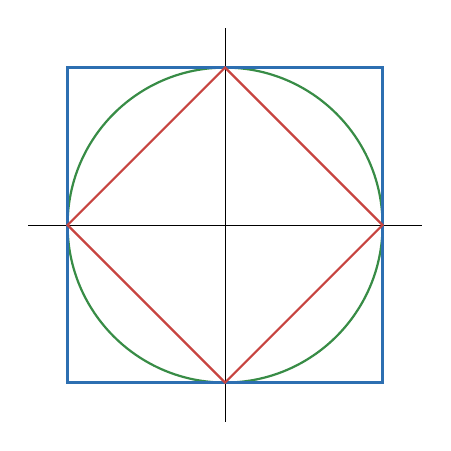
\begin{tikzpicture}
		\draw (-2.5, 0) -- (2.5, 0) ;
		\draw (0, -2.5) -- (0, 2.5) ;
		\draw[myg,thick] (0,0) circle (2cm);
		\draw[myb,thick] (-2,2) -- (2,2) -- (2,-2) -- (-2,-2) -- cycle;
		\draw[myr,thick] (2,0) -- (0,-2) -- (-2,0) -- (0,2) --cycle;
	\end{tikzpicture}
\end{center}

draw an ordinary circle around the origin then no matter how small the circle the points of the sequence are eventually land inside the circle. If instead of that circle can same be said for diamond w.r.t norm 2. Then i can take circle that is inside that diamond. Same is true for $\infty-$norm. Hence convergence with respect to all norm $1$ and norm 2 and even $\infty$ results for convergence.






Now there is no reason why we can not consider a norm on an infinite dimensional vector space. It will work. Perhaps i can define only for some sequences where the morm converges. \ex{}{Suppose for set of all bounded infinite sequences a vector space because every number in a vector is less than some number so if you add two vectors then add the bound and if you scale then scale the bound. Now the $\infty$ norm works on that.

	Now suppose you take all continuous real valued functions on closed interval $[0,1]$, such a function is bounded and this is a vector space and we can define $\infty-$norm even for that because for all $f$ in this space attains its maximum value so just take that maximum value. Its an extremely infinite dimensional space.


}

\begin{note}
	$\bbR^{\infty}$ is the space of all sequences.
\end{note}

\qs{}{\label{exs2}Modify the above proof for field $\bbC$}
\qs{}{\label{exs3}Show that the following are normed linear spaces.\begin{enumerate}[label=(\alph*)]
		\item $l^{\infty}=$ Set of all bounded infinite sequences $(x_1,x_2,\cdots)$ $x_i\in\bbR$ with norm $\|x\|=\sup |x_i|$
		\item $C[0,1]=$ Set of all continuous functions $[0,1]\to \bbR$ with norm $\|f\|=\sup\limits_{x\in[0,1]}|f(x)|$
	\end{enumerate}
}
\section{Limit of a Sequence}
\dfn{Limit of Sequence in Normed Linear Space}{A sequence  $\{s_n\}$ in a normed linear space $V$ converge to $s$ means $\forall$ real number $\eps>0$ $\exists$ natural number $N$ such that for $\forall\ n>N$ $\|s-s_n\|<\eps$}
\section{Continuity}
\dfn{Continuity in Normed Linear Space}{Let $S$ be a subset of $V$ and $f:\ S\to W$ where $V,W$ are normed linear space. $f$ is continuous at $v\in V$ means $\forall$ $\eps>0$, $\exists$ $\delta>0$, st whenever $\|x-v\|<\delta$ for $x\in S$ one has $\|f(x)-f(v)\|<\eps$}
Distance in a normed linear space for $x,y\in V$ is $$d(x,y)=\|x,y\|$$ Hence properties of this $d$ are\begin{enumerate}[label=\bfseries\tiny\protect\circled{\small\arabic*}]
	\item[\ref{n:1}] \label{m:1} $d(x,y)=0 \iff x=y$
	\item[\ref{n:2}] \label{m:2} $d(\lambda x,\lambda y)=|\lambda|d(x,y)$ for any scalar $\lambda$
	\item[\ref{n:3}] \label{m:3} $d(u,v)+d(u,v)\geq d(u,w)$
\end{enumerate}


\chapter{Metric Space}
\section{Definition}
\dfn{Metric Space $\bs{X}$}{A set $X$ with a function $d\:\ X\times X\to\bbR_{\geq 0}$ such that\begin{enumerate}[label=\bfseries\tiny\protect\circled{\small\arabic*}]
		\item $d(x,y)=0\iff x=y$
		\item $d(x,y)=d(y,x)$
		\item $d(x,z)\leq d(x,y)+d(y,z)$
	\end{enumerate}}
Notice that there is no homogeneity condition, and it does ot make sense as we don't have a field. In fact there is no notion of addition. But the condition \ref{n:1} of norm has to be satisfied by this distance. Also we don't have a translational condition i.e. distance between $x,y$ and distance  between $x+v,y+v$ has to be same. Hence
\begin{note}
	A metric space need not be a vector space. So it doesn't need a zero, or a notion of addition or scalar multiplication.
\end{note}
If I take a metric space and take any subset of it. And those three conditions of distance functions are still satisfied.
\begin{note}
	Any subset of metric space is a metric space under the same distance function.
\end{note}
\section{Open and Closed Ball and Set}
\dfn{Open Ball and Closed Ball in a Metric Space}{An open ball of radius $r$ with center $c\in X$ in a metric space $X$ is $$B_r(c)=\{x\in X\mid d(c,x)< r\}$$and a closed ball is $$\overline{B_r(c)}=\{x\in X\mid d(c,x)\leq r\}$$}
\pagebreak
\dfn{Open Set and Closed Ball in a Metric Space}{An open set in a metric space $X$ is one of the form of union of some open balls and a closed set in a metric space $X$ is one of the form of $X\setminus $some open sets}


\nt{We will do topology in Normed Linear Space  (Mainly $\bbR^n$ and occasionally $\bbC^n$)using the language of Metric Space}
\ex{Open Set and Close Set}{
	\begin{tabular}{rl}
		Open Set:   & $\bullet$ $\phi$                                              \\
		            & $\bullet$ $\bigcup\limits_{x\in X}B_r(x)$ (Any $r>0$ will do) \\[3mm]
		            & $\bullet$ $B_r(x)$ is open                                    \\
		Closed Set: & $\bullet$ $X,\ \phi$                                          \\
		            & $\bullet$ $\overline{B_r(x)}$                                 \\
		            & $x-$axis $\cup$ $y-$axis
	\end{tabular}}

\qs{}{Is the set ${x-}$axis${\setminus\{\text{Origin}\}}$ a closed set}\sol We have to take its complement and check whether that set is a open set i.e. if it is a union of open balls

Now this works well for points which are above or below the $x-$axis. But for origin no matter how small the ball we take it willl have points from $x-$axis. Hence the set is not a closed set.
\qs{}{Any continuous path in $\bbR^2$ is closed where $\text{path}=f:[0,1]\to\bbR^2$}
\sol This is true. To be proved later.\\
Analogous to: For continuous function $f:[0,1]\to\bbR$, the image is a closed interval
\qs{}{If i take $X=x-$axis $\cup\ y-$axis then is it open}
\sol Yes because here the space is only the union of those two axis. So any ball would be like a cross or line but it just as the metric space given to us. [It is open for this metric space but not open in $\bbR^2$]
\nt{If $S\subset X$, then $S$ itself has a collection of open sets of $S$ by containing $S$ as a metric space.}
\dfn{Neighborhood}{For a point $x$ in metric space $X$, a neighborhood of $x$ is a set $N$ such that $x\in $an open set $U\subset N$

	\vspace*{2mm}
	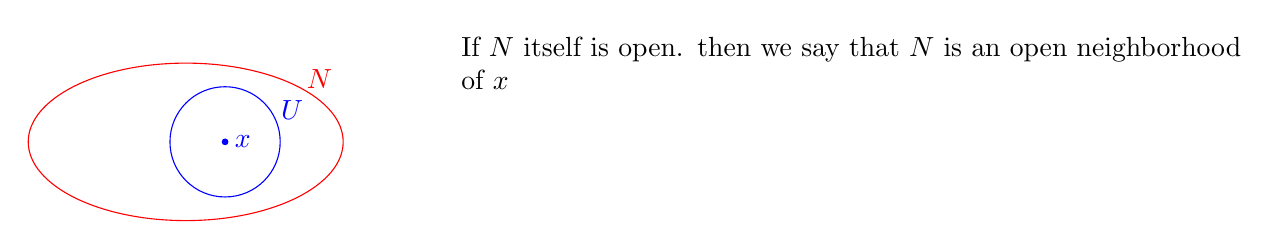
\begin{tikzpicture}
		\draw[red] (0.5,0) circle [x radius=2cm, y radius=1cm] ;
		\draw (2.2,0.8) node[red]{$N$};
		\draw [blue] (1,0) circle (7mm) ;
		\filldraw[blue] (1,0) circle (1pt) node[anchor=west]{$x$};
		\draw (1.85,0.4) node[blue]{$U$};
		\node[black,text width=10cm] at (9,1){If $N$ itself is open. then we say that $N$ is an open neighborhood of $x$};
	\end{tikzpicture}}


\thm{}{If $x\in$ open set $V$ then $\exists$ $\delta>0$ such that $B_{\delta}(x)\subset V$}

\begin{myproof}By openness of $V$, $x\in B_r(u)\subset V$
	\begin{center}
		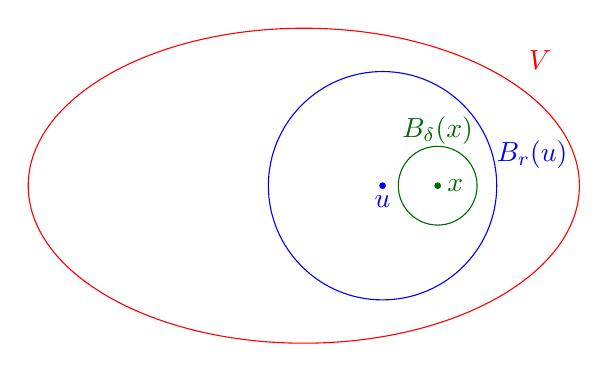
\begin{tikzpicture}
			\draw[red] (0,0) circle [x radius=3.5cm, y radius=2cm] ;
			\draw (3,1.6) node[red]{$V$};
			\draw [blue] (1,0) circle (1.45cm) ;
			\filldraw[blue] (1,0) circle (1pt) node[anchor=north]{$u$};
			\draw (2.9,0.4) node[blue]{$B_r(u)$};
			\draw [green!40!black] (1.7,0) circle (0.5cm) node [yshift=0.7cm]{$B_{\delta}(x)$} ;
			\filldraw[green!40!black] (1.7,0) circle (1pt) node[anchor=west]{$x$};
		\end{tikzpicture}
	\end{center}

	Given $x\in B_r(u)\subset V$, we want $\delta>0$ such that $x\in B_{\delta} (x)\subset B_r(u)\subset V$. Let $d=d(u,x)$. Choose $\delta $ such that $d+\delta<r$ (e.g. $\delta<\frac{r-d}{2}$)

	If $y\in B_{\delta}(x)$ we will be done by showing that $d(u,y)<r$ but $$d(u,y)\leq d(u,x)+d(x,y)<d+\delta<r$$
\end{myproof}
\nt{$V$ is open $\iff\bigcup\limits_{x\in V}B_r(x)$ (where $r$ depends on $x$)}
\thm{}{Let $X$ be a metric space.\begin{enumerate}
		\item Union of open sets is open
		\item Intersection of two open sets is open
	\end{enumerate}Analogues to these as we are just taking complement of the open sets
	\begin{enumerate}[label=\arabic*$'$.]
		\item Arbitrary intersection of closed sets is closed
		\item Finite union of closed sets is closed.
	\end{enumerate}

}

\begin{myproof}
	\begin{enumerate}
		\item Let $\{V_{\alpha}\}_{\alpha\in I}$ be a collection of open sets where $I$ is an index set. We want ti show $\bigcup\limits_{\alpha\in I}V_{\alpha}$ is open in $X$. Since each $V_{\alpha}$ is open $V_{\alpha}=\bigcup\limits_{\beta \in J_{\alpha}} B_{r_{\beta}}(c_{\beta})$ Then \begin{align*}
			      \bigcup\limits_{\alpha\in I} V_{\alpha} & =\bigcup\limits_{\alpha\in I}\bigcup\limits_{\beta \in J_{\alpha}}B_{r_{\beta}}(c_{\beta}) \\
			                                             & =\bigcup\limits_{\beta \in \sqcup J_{\alpha}}B_{r_{\beta}}(c_{\beta})
		      \end{align*} which is still a union of balls
		      \Qed
		\item \setlength{\parindent}{1cm}The statement implies intersection of finite number of open sets is open. We can prove this by induction.

		      We will do by showing that for each $x\in V_1\cap V_2$ $\exists$ $r>0$ s.t. $B_r(x)\subset V_1\cap V_2$

		      \begin{center}
			      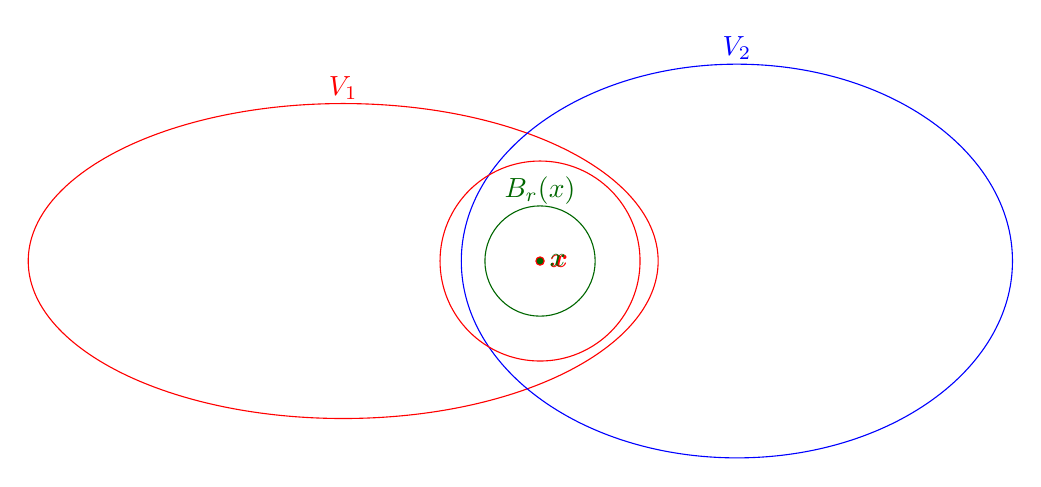
\begin{tikzpicture}
				      \draw[red] (0,0) circle [x radius=4cm, y radius=2cm] ;
				      \draw[blue] (5,0) circle [x radius=3.5cm, y radius=2.5cm] ;
				      \draw (0,2.2) node[red]{$V_1$};
				      \draw (5,2.7) node[blue]{$V_2$};
				      \draw [red] (2.5,0) circle (1.27cm) ;
				      \filldraw[red] (2.5,0) circle (1.5pt) node[anchor=west]{$\bs{x}$};
				      %	\draw [blue] (2.5,0) circle (0.85cm) node [yshift=1cm]{$B_{r}(x)$} ;
				      \draw [green!40!black] (2.5,0) circle (0.7cm) node [yshift=0.9cm]{$B_{r}(x)$} ;
				      \filldraw[green!40!black] (2.5,0) circle (1pt) node[anchor=west]{$x$};
			      \end{tikzpicture}
		      \end{center}
		      As $x\in V_1$ $\exists$ $r_1$ such that $x\in B_{r_1}(x)\subset V_1$. Similarly $x\in V_2$ $\exists$ $r_2$ such that $x\in B_{r_2}(x)\subset V_2$. Take $r=\min\{r_1,r_2\}$. Thus we have $x\in B_r(x)\subset V_1\cap V_2$

	\end{enumerate}
	The second part for closed sets are left as exercise
\end{myproof}

\section{Topological Space}
\dfn{Topological Space}{\label{topological-space}A topological space is a set $X$ together with a collection of subsets of $X$ (i.e. a subset of the power set of $X$) that is closed under taking arbitrary unions and finite intersections. This collection is called a topology on $X$}


\nt{Union means $\bigcup\limits_{\alpha\in I}S_{\alpha}=\{x\in X\mid \exists\ \alpha\text{ s.t. }x\in S_{\alpha}\}$\\
Intersection means $\bigcap\limits_{\alpha\in I}S_{\alpha}=\{x\in X\mid \forall\alpha,\ x\in S_{\alpha}\}$}

\qs{}{  Suppose i have a topological space $X$ under given some topology. Is the entire set open ? And that the empty set is open ?
}\sol If $I=\phi$, $\bigcup\limits_{\alpha\in I}S_{\alpha}=\{x\in X\mid \exists\ \alpha\in I\text{ s.t. }x\in S_{\alpha}\}$  gives $\phi$
and\\ $\bigcap\limits_{\alpha\in I}S_{\alpha}=\{x\in X\mid \forall\alpha\in I,\ x\in S_{\alpha}\}$  gives $X$ because $\forall\ \alpha\in I$ condition is vacuously true for each $x\in X$.
\nt{Intersection of empty families are not defined in set theory. This brings a very important point. In a set theory you have to have a universe. (Set theory have to avoid paradoxes, Russel Paradox) At the beginning you construct a large enough universe and you taking subsets only from that universe. Notice all subsets we are considering here are subsets of $X$ and here we defined how we union and intersection mean. Though it still this asks what our axioms of set theory. So you can change the part of the definition of \hyperref[topological-space]{topological space} like this ``$\dots$with a collection of subsets of $X$ including the empty set and the whole space$\dots$"} (If you don't like this as it is)
\nt{If $S$ is a subset of metric space $X$, then $S$ is itself a metric space and as such open/closed sets as subsets of metric space}
\qs{}{Is there any connection between being open in $X$ and being open in $S$ (Similar question for closed)}

\sol Let $x\in S$. Now, Ball of radius $r$ in $S = S\cap$ Ball of radius $r$ in $X$. Therefore \begin{align*}
	\text{Open Set in } S & =\bigcup \text{ Balls in }S                    \\
	                      & =\bigcup\ (\text{Balls in }X\cap S)            \\
	                      & =\left(\bigcup \text{ Balls in }X\right)\cap S \\
	                      & =\text{Open set }X\cap S
\end{align*}
Part 2 is left as exercise

\cor{}{
	If $S\subset X$ is open in $X$ then a subset $T$ of $S$ is open in $S\iff $ $T$ is open in $X$}

\cor{}{
	If $S\subset X$ is closed in $X$ then a subset $T$ of $S$ is closed in $S\iff $ $T$ is closed in $X$}

\dfn{Subspace of a Topological Space $X$}{For any subset $S$ of a topological space $X$, the collection $S\cap U$, $U$ open in $X$  is called a subspace.}
\qs{}{Prove that subspace of a metric space $X$ defines a topology on $X$}
\wc{}{ If $x\in $ open $V$ then there exists $r>0$ such that $x\in B_r(x)\subset V$
	\begin{center}
		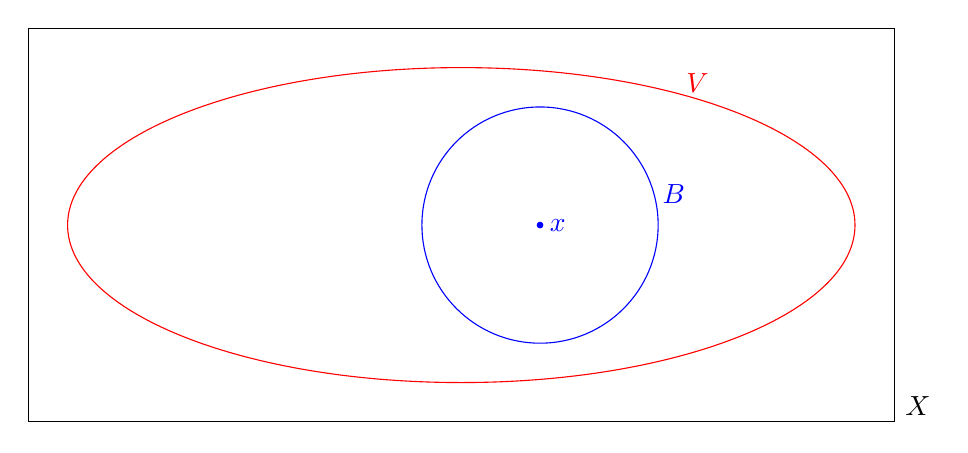
\begin{tikzpicture}
			\draw (-5.5,2.5) rectangle (5.5,-2.5) node[xshift=3mm,yshift=2mm]{$X$};
			\draw[red] (0,0) circle [x radius=5cm, y radius=2cm] ;
			\draw (3,1.8) node[red]{$V$};
			\draw [blue] (1,0) circle (1.5cm) ;
			\filldraw[blue] (1,0) circle (1pt) node[anchor=west]{$x$};
			\draw (2.7,0.4) node[blue]{$B$};
			%\node[black,text width=10cm] at (9,1){If $N$ itseld is open. then we say that $N$ is an open neighbourhood of $x$};
		\end{tikzpicture}
	\end{center}
	\textbf{Idea: }Why not we take $r=\inf \{\text{distance from }x\text{ to boundary of ball } B\}$.

	Now we first have to ensure $r>0$. Suppose that's true.

	Then we have to define boundary. What is boundary, We can give a reasonable definition (Boundary has already a definition but we don't know that for now). Let boundary of $B=\{x\in X\mid d(c,x)=\delta\}$ Now this definition is not proper for our purpose.Because if we take union of all balls in $V$ then we will have lots of points as boundary but part of them should not be considered as boundary. Even if we take this definition.

	Then the big question comes/ We are taking a infimum of a certain set of real numbers. The very first question arises is whether this set is nonempty. For example if we take $B$ to be the metric space it self we have no boundary.
	\tcblower
	Questions which come thorough this.
	\begin{itemize}
		\item Is there a meaningful way to define boundary
		\item Can we modify the idea
	\end{itemize}
}


\chapter{Continuity in Metric Space}
\section{Limit Point and Closure}

\dfn{Limit Point}{$S\subset X$ is a metric space. We say that $x\in X$ is a limit point of $S$ if $\exists$ a sequence $\{s_n\}$ with all $s_n\in S\setminus\{x\}$ such that $s_n\to x$ (each $s_n$ is different from $x$)}

\begin{Theorem}{}{limitpoint}
	$x$ is a limit point of $S$ $\iff$ every neighborhood of $x$ in $X$ contains a point of $S$ other than $S$.
\end{Theorem}
\begin{myproof}
	\subsubsection*{If Part:}
	Let $x$ be a limit point of $S$. Therefore take a sequence $\{s_n\}$ in $S\setminus \{x\}  $ with $s_n\to x$ .

	To prove what we want it is enough to show that $B_r(x)\cap S$ contains a point other than $x$. As $s_n \to x$, $\exists $ $N$ s.t.  $\forall $ $n>N$ $d(x,s_n)<r$ i.e. $s_n\in B_r(x)$. In particular $s_n]in B_r(x)\cap (S\setminus \{x\})$
	\subsubsection*{Only If Part:}
	We need to produce  a sequence $\{s_n\} \in S\setminus \{x\}$ with $\lim s_n=x$. Take $s_n\in B_{\frac1n}(x)\cap (S\setminus \{x\})$ See that $\lim\limits_{n\to \infty}s_n=x$. This is essentially because $\frac1n\to 0$.

	Complete the rest of the proof.

\end{myproof}
\dfn{Closure}{Given a topological space $X$ and $S\subset X$, the closure of the set $S$ is $\overline{S}$ the smallest closed set containing $S$.}
\begin{Theorem}{}{closure}
	\begin{tabular}{rl}
		$\overline{S} $ & $=\text{Smallest closed set of } X\text{ containing }S $                                     = \setword{A}{A}                \\
		                & $ =S\cup (\text{limit points of }S)$                                                         =                \setword{B}{B} \\
		                & $=\{x\in X\mid x=\lim\limits_{n\to \infty} \text{ for some sequence }\{s_n\} \text{ in }S\}$ =                \setword{C}{C} \\
		                & $=\{x\in X\mid \text{Every neighborhood of }x\text{ intersects }S\}$                         =                \setword{D}{D}
	\end{tabular}
\end{Theorem}
\begin{myproof}
	\subsubsection*{$\bs{A\subset D}$}
	\begin{tabular}{l}\hspace{1.5cm}$A^c=\bigcup$ (All open set $V$ s.t. $V\cap S=\phi$) \\ \hspace{1.5cm}$D^c=\{x\in X\mid \exists \text{ open neighborhood of }x,B\text{ s.t. }B\cap S=\phi \}$\end{tabular}

	\setlength{\parindent}{0cm}Clearly for all $x\in D^c$, $x\in A^c$. Hence $D^c\subset A^c\implies A \subset D$\setlength{\parindent}{1cm}
	\subsubsection*{$\bs{D\subset B}$}
	Take $x\in D$. Suppose $x\notin S$. Now any neighborhood of $x$ intersects $S$ in a point hence it has to be a different point from $x$ since $x\notin S$. Therefore $x$ is a limit point of $S$. $D\subset B$
	\subsubsection*{$\bs{B\subset C}$}
	If $x\in S$ then take a sequence

\end{myproof}

\qs{}{What does it mean to be smallest closed set containing the set $S$ here ?}
\sol $\bigcap$ All closed sets containing $S$ is automatically closed and hence the smallest closed set containing $S$.
\begin{myproof}
	For proof of \hyperref[th:closure]{Theorem \ref{th:closure}} notice \ref{A},\ref{B},\ref{C},\ref{D} all contains $S$ (obvious).
	\nt{We don't need to show \ref{B},\ref{C},\ref{D} are closed. We can also take the sets element wise and show each set is a subset of the other. This may simplify our way of proof. (exercise)}

	Now see $A$ and $D$ completely deal with topology. \ref{A} is about closed sets and \ref{D} is about open sets. So \ref{A} and \ref{D} close to each other. Now by the \ref{th:limitpoint} we have equivalence of \ref{C} and \ref{D}. So we can prove like this
	$$\ref{A}\iff\ref{D}\iff\ref{B}\ \&\ \ref{C}$$Left as exercise
\end{myproof}\nt{For these kind of proofs instead of looking for the most efficient way try to find a path that allows you to go from anywhere to anywhere}
\section{Continuity}
\dfn{Continuity}{$f:X\to Y$ function between metric spaces is continuous at $a\in X$ if $\forall$ $\eps>0$ $\exists$ $\delta>0$ s.t. \begin{align*}
		d(x,a)<\delta      & \implies d(f(a),f(x))<\eps      \\
		\Updownarrow\qquad & \qquad\qquad\qquad \Updownarrow \\
		x\in B_{\delta}(x) & \implies f(x)\in B_{\eps}(f(a))
	\end{align*}}
\setlength{\parindent}{0cm}That means $f^{-1}$(Any ball around $f(a)$) $\supset$ Ball around $a$.\setlength{\parindent}{1cm}

So $f:X\to Y$ is continuous at all points $\iff$ $f^{-1}(\text{Any ball intersecting the range})\supset $ A ball
\nt{We can not say $f^{-1}(\text{Any ball})$ because because we need a ball that contains a point in the range
}
\begin{Theorem}{}{cont:invofopen}
	$f$ is continuous $\iff$ $f^{-1}(\text{Any open set in }Y)$ is open in $X$
\end{Theorem}
\begin{myproof}
	\subsubsection*{If Part:-}
	It is enough to show $f^{-1}(\text{Any ball})$ is open on $X$ because $f^{-1}$ preserves unions $f^{-1}\left(\bigcup\limits_{\alpha}V_{\alpha}\right)=\bigcup\limits_{\alpha}\left(f^{-1}(V_{\alpha})\right)$

	Let $B$ is any open set (as its conceptually simpler to take open set here instead of a ball) in $Y$. Let $a\in f^{-1}(B)$. Hence we can say $f(a)\in B$. Since $B$ is an open set we can say there is a ball $B_{\eps}(f(a))\subset B$. Since $f$ is continuous $\exists$ $\delta $ such that $f(x)\in B_{\eps}(f(a))$ whenever $x\in B_{\delta}(a)$. Now $f^{-1}(B)\supset f^{-1}\Big(B_{\eps}(f(a))\big)\supset B_{\delta}(a)$ Hence $f^{-1} (B)$ is open.

	\subsubsection*{Only If Part:-}
	Lets prove continuity ar $a\in X$. We are given that $f^{-1}\Big(B_{\eps}(f(a))\Big)$ is open and obviously contains $a$. Therefore $f^{-1}\Big(B_{\eps}\big(f(a)\big)\Big)$ contains a ball around $a$. Take $\delta=$ Radius of the ball.
\end{myproof}

\qs{}{
	For a metric space $X$, show that $\overline{S} =\{x\in X\mid \lim\limits_{n\to\infty}s_n=x\}$ for some sequence $\{s_n\}$ in $S$.}

\qs{}{For a function $f:X\to Y$ between metric spaces, show that the followings are equivalent.\begin{enumerate}
		\item $f$ is continuous
		\item $f^{-1}(\text{Open Set)}$ is open
		\item $f^{-1}(\text{Closed Set})$ is closed
		\item \label{itm:wrong} $f(\overline{S})=\overline{f(S)}$
		\item $x_n\to x \implies f(x_n)\to f(x)$
	\end{enumerate}
	One or more of the above are wrong so check if they are true and if not then find the true statement.}
\sol \ref{itm:wrong} is wrong. How to correct and rest is left as exercise
\qs{}{For $f:X\to Y$ any set map\begin{enumerate}[label=(\roman*)]
		\item $f^{-1}$ preserves unions, intersections, complements
		\item Is there any condition on $f$ under which $f$ possesses the property above ?
	\end{enumerate}}
\ex{Continuous Function}{\begin{enumerate}
		\item Any constant function.
		\item $X\xrightarrow{f} Y\xrightarrow{g}Z$ $f,g\text{ continuous} \implies g\cdot f$ is continuous
		\item Is $ S\subset X$ then $S\xrightarrow{\text{Inclusion}}X$ is continuous
		\item Projection $\underset{(x_1,x_2,\cdots,x_n)\mapsto x_i}{\bbR^n\to \bbR}$

		      More generally for example $\underset{(x,y,z)\mapsto(x,x,y,y)}{\bbR^3\to \bbR^4}$
		\item Map from metric space to euclidean space.$$\begin{rcases*}
				      X\to \bbR^n \\
				      x\mapsto (f_1(x),f_2(x),\cdots,f_n(x))
			      \end{rcases*}\substack{{f\text{ is continuous}}\\ {\iff} \\ {\text{each }f_i\text{is continuous}}}$$
		\item $\bbR\times \bbR\to\bbR: \ (x,y)\mapsto x\pm y,xy$ are continuous.

		      We need to prove $x_n\to x$ and $y_n\to y$ in $\bbR\implies \begin{cases*}
				      x_n\pm y_n\to x\pm y \\ x_ny_n \to xy
			      \end{cases*}$

		      $\bbR\setminus\{0\}\to \bbR:\ x\mapsto \frac1x$ is continuous
		\item sum and product of two continuous real valued function on $X$ are continuous
		      $$f,g:X\xrightarrow{f,g}\bbR\text{ continuous}\implies \underset{x}{X}\underset{\longmapsto}{\xrightarrow{f,g}}\underset{(f(x),g(x))}{\bbR\times\bbR}\xrightarrow{+}
			      \bbR$$ $$f:X\to\bbR\implies \frac1f:\underbrace{X\setminus f^{-1}(0)}_{\text{open set in }X}\to \bbR\text{ is continuous}$$ $\{0\}$ is closed in $\bbR$, so $f^{-1}(0)$ is closed in $X$ by  continuity of $f$\parinn

		      Therefore any polynomial in continuous real valued functions on $X$ is continuous.
		\item \textbf{Special Case:} \begin{itemize}
			      \item \parinn $\bbR^n\xrightarrow{T}\bbR^m$ linear map is continuous where $(x_1,x_2,\cdots,x_n)\longmapsto(a_{11}x_1+\cdots+a_{1n}x_n,a_{21}x_1+\cdots+a_{2n}x_n,\cdots,a_{m1}x_1+\cdots+a_{mn}x_n)$

			            Matrix of $T=\begin{bmatrix}
					            a_{11} & a_{12} & \cdots & a_{1n} \\
					            a_{21} & a_{22} & \cdots & a_{2n} \\
					            \vdots & \vdots & \ddots & \vdots \\
					            a_{m1} & a_{m2} & \cdots & a_{mn}
				            \end{bmatrix}$
			      \item  $\underset{A}{M_{n\times n}(\bbR)}\underset{\longmapsto}{\to} \underset{det(A)}{\bbR}$ is continuous

			            $\frac1{\text{det}}:GL_n(\bbR)\to\bbR$ \parinn

			            Here $M_{n\times n}$ is a vector space of dimension $n^2$ in which $GL_n(\bbR)=\{A\mid \det(A)\neq 0\}$ is an open set.

			      \item $\underset{A\longmapsto A^{-1}}{ GL_n(\bbR) \to GL_n(\bbR) }$ is continuous.

		      \end{itemize}
		\item Any norm $(f)$ on $\bbR^n$ is uniformly continuous w.r.t usual topology on $\bbR^n$ i.e. $f:\bbR^n\to\bbR$ is continuous w.r.t usual norms ($\norm=p0$norm for $p=1,2,\infty$) on $\bbR^n(\norm)$ and $\bbR(|\cdot|)$
	\end{enumerate}
}
\begin{Theorem}{}{}
	Any norm $(f)$ on $\bbR^n$ is uniformly continuous w.r.t usual topology on $\bbR^n$ i.e. $\forall\ \eps>0$ $\forall\ x,y\in\bbR^n\ \exists\ \delta>0$ s.t. $\|x-y\|<\delta\implies |f(x)-f(y)|<\eps$
\end{Theorem}
\begin{myproof}
	$$\begin{rcases*}
			f(x)\leq f(y)+f(x-y) \\ \qquad \qquad\qquad \qquad \parallel\\ f(y)\leq f(x)+f(y-x)
		\end{rcases*}|f(x)-f(y)|\leq f(x-y)$$Let $x=\sum x_ie_i$ and $y=\sum y_ie_i$ where $\{e_i\}$ is the standard basis of $\bbR^n$.

	$$f(x-y)=f\left(\sum (x_i-y_i)e_i\right)\leq \sum f\left((x_i-y_i)e_i\right)=|x_i-y_i|f(e_i)$$ Notice $\sum|x_i-y_i|=\|x-y\|_1$. Let $M=\max\{f(e_i)\}$ Then $$|f(x)-f(y)|\leq f(x-y)\leq M\|x-y\|_1$$

	Thus $\|x-y\|<\frac{\eps}{M}\implies |f(x)-f(y)|<\eps$
\end{myproof}


\chapter{Equivalence of Norms}
We back to Normed Linear Space for a little while.

In $\bbR^n$, $u=(u_1,u_2,\cdots,u_n)$ where each $u_i\in \bbR$. we have \hyperref[norm]{$p-$norm}: $\|u\|_p=\left(\sum\limits_i|u_i|^p\right)^{\frac1p}$ where $1\leq p\leq \infty$. Balls in $\bbR^2$ w.r.t. $\textcolor{myr}{\norm_1}$, $\textcolor{myg}{\norm_2}$, $\textcolor{myb}{\inorm}$.

\begin{center}
	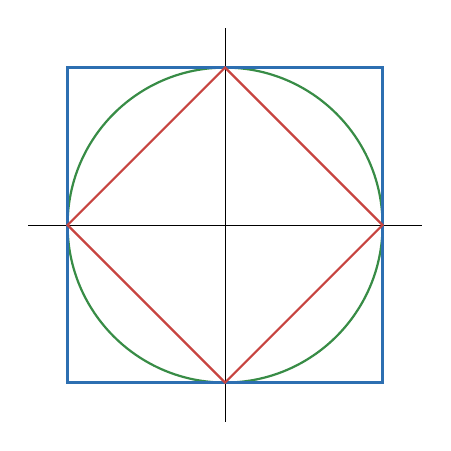
\begin{tikzpicture}
		\draw (-2.5, 0) -- (2.5, 0) ;
		\draw (0, -2.5) -- (0, 2.5) ;
		\draw[myg,thick] (0,0) circle (2cm);
		\draw[myb,thick] (-2,2) -- (2,2) -- (2,-2) -- (-2,-2) -- cycle;
		\draw[myr,thick] (2,0) -- (0,-2) -- (-2,0) -- (0,2) --cycle;
	\end{tikzpicture}
\end{center}

\underline{Observe}: A set $V$ in $\bbR^2$ is
\begin{center}
	\begin{tabular}{lcl}
		open w.r.t. $\norm_1$ & $\iff$ & $V=\bigcup\limits_{u\in V}$ Box in $V$ centered box     \\
		open w.r.t. $\norm_2$ & $\iff$ & $V=\bigcup\limits_{u\in V}$ Diamond in $V$ centered box \\
		open w.r.t. $\inorm$  & $\iff$ & $V=\bigcup\limits_{u\in V}$ Circle in $V$ centered box
	\end{tabular}
\end{center}
\dfnc{Equivalence of Norms}{Suppose $\norm$, $\norm'$ are two norms in vector space $V$, We say that the two norms are equivalent if there are constants $\alpha,\beta>0$ s.t. $$\alpha\|x\|'\leq \|x\|\leq \beta\|x\|'$$}
\ex{Norm Equivalence}{\begin{enumerate}
		\item \textbf{$\bs{p=\infty}$ and $\bs{p=1}$}

		      $\|x\|_{\infty}=\max\{|x_i|\mid 1\leq i\leq n\}\leq \|x\|_1=\sum\limits_i |x_i|$

		      $\|x\|_{\infty}\geq $ each $|x_i|\implies n\|x\|_{\infty}\geq \|x\|_1$

		      Hence $$\|x\|_{\infty}|\leq \|x\|_1\leq n\|x\|_{\infty}\text{ and }\frac1n\|x\|_1\leq \|x\|_{\infty}\leq \|x\|_1$$
		\item \textbf{$\bs{p=\infty}$ and $\bs{p=2}$}
		      $$\|x\|_{\infty}\leq \|x\|_2\leq \sqrt{n}\|x\|_{\infty}$$
	\end{enumerate}}
\begin{theorem}{}{}
	All norms on a finite dimensional vector space are equivalent
\end{theorem}
\begin{myproof}
	Proved in \hyperref[th:all norms equiv]{Theorem \ref{th:all norms equiv}}
\end{myproof}
\begin{theorem}{}{}
	Suppose $\norm$ and $\norm'$ are equivalent on a vector space $V$. Then \begin{enumerate}[label=(\roman*)]
		\item $\{x_n\}\to x$ w.r.t. $\norm\iff \{x_n\}\to x$ w.r.t $\norm'$
		\item $S\subset V$ is open w.r.t $\norm\iff$ $S$ is open w.r.t $\norm'$
	\end{enumerate}
\end{theorem}
\begin{myproof}
	For both proofs if we just prove one direction the we are done actually since we can just replace
	the words to prove for opposite direction,
	\begin{enumerate}[label=(\roman*)]
		\item \parinn\subsubsection{If Part:-}
		      Since $\norm,\norm^{\prime}$ are equivalent we have $\exists\ \alpha, \beta$ such that $\alpha\|x\|^{\prime} \leq\|x\| \leq \beta\|x\|^{\prime}$. So if we show $\alpha\left\|x_{n}-x\right\|<\left\|x_{n}-x\right\|<\alpha \epsilon$ we are done.

		      Let $\{x_{n}\} \to x$ w.r.t $\norm$ i.e. $\forall\ \epsilon>0\ \exists\ N$ s.t. $\forall\ n>N\ \left\|x_{n}-x\right\|<\alpha \epsilon$. Hence we have $\alpha\left\|x_{n}-x\right\|^{\prime}<\alpha \epsilon$. Hence $\forall \ \epsilon>0\ \exists\ N$ such that $\forall\ n>N\ \left\|x_{n}-x\right\|^{\prime}<\epsilon$\Qed

		\item \subsubsection{Only If Part:-}\parinn
		      $V$ is open w.r.t $\norm\iff\bigcup\limits_{x\in V}B_r(x)$ and $V'$ is open w.r.t $\norm'\iff\bigcup\limits_{x\in V}B'_r(x)$

		      Now we have $$B_r(x)=\{y\mid \|y-x\|<r\}\text{ and } B'_r(x)=\{y\mid \|y-x\|'<s\}$$Hence by equivalence of the norms for any $v$ $$\alpha \|v\|'\leq \|v\|\leq \beta\|v\|'$$ Since $\|v\|<r$ we have $$\|v\|'\leq \frac{r}{\beta}\implies B'_{\frac{r}{\beta}}(x)\subset B_r(x)$$
	\end{enumerate}

\end{myproof}
\begin{corollary}{}{}
	$p=1$ and $p=\infty$ on $\bbR^n$ (and $\bbC^n$) give the same topology as $p=2$ norm
\end{corollary}
\begin{corollary}{}{}
	Let $x_m$ be a square in $\bbR^n$. $\overline{x_m}=(x_{m_1},x_{m_2},\cdots,x_{m_n})$. Then $\{\overline{x_m}\}\to x=(x_1,x_2,\cdots,x_n)$ w.r.t $\norm_2\iff \{x_{m_i}\}\to x_i$ in $\bbR$ for each $i$.
\end{corollary}
\nt{We can check this w.r.t $\inorm$
	\begin{center}
		\begin{tabular}{rcl}
			$\overline{x_m}\to \overline{x}$ w.r.t $\inorm$ & $\iff$ & $\forall\ \eps>0\ \exists \ N$ s.t. $\forall\ m>N$ $\max\{|x_{m_i}-x_i| \mid 1\leq i\leq n\}$ \\
			                                                & $\iff$ & each $|x_{m_i}-x_i|<\eps\ \forall\ i$                                                         \\
			                                                & $\iff$ & $\lim\limits_{n\to \infty}x_{m_i}=x_i\ \forall \ i$
		\end{tabular}
	\end{center}
}

\chapter{Compactness}
\section{Sequentially Compact}
\dfn{Sequentially Compact}{Let $(X,d)$ be a metric space. $X$ is called sequentially compact if every sequence in $X$ has a convergent subsequence. (Often applied to a subset $S$ of $X$)}
\nt{For $S$ to be sequentially compact the limit of subsequence must be in $S$}
\dfn{Boundedness}{A subset $S$ of $(X, d)$ is bounded if $S \subset B_r(x)$ for some $x \in X$ and $r > 0$}
\nt{Boundedness depends on the metric but if two metrics are ``equivalent" analogous to norms)}
\begin{Theorem}{}{}
	A subset $K$ of $\bbR^n$ is sequentially compact $\iff$ $K$ is closed and bounded
\end{Theorem}
\begin{myproof}
	Proof in steps
	\begin{enumerate}
		\item \label{hnbsc: step 1}\subsubsection{A closed interval $\bs{[a, b]}$ in
			      $\bbR$ is sequentially compact}\parinn
		      \begin{myproof}
			      Given a sequence $x_1 , x_2 , \cdots$  in $\bbR$ in $[a, b]$ we can extract a monotonic subsequence as follows:

			      We call $x_i$ to be a peak if $x_i > x_j$ $\forall\ j > i$. Now there are two cases. If number of peaks is infinite then the next peak comes after the previous one so smaller than the previous one. So its a strictly decreasing sequence. If number of peaks are finite then at some point we cant find a peak with this property that means no matter which term i peak there is at least one term after that which is greater than or equal to that term. $y_1 = $a term after the last peak. and $y_{i+1} = $a term after $y_i$ such that $y_{i+1} \geq y_i$. Hence $y_1 , y_2 ,\cdots$ is a weakly increasing	sequence.

			      When $\{x_n\}$ contained in $[a, b]$ by boundedness of the monotonic subsequence, it converges to its sup/inf and the limit is in $[a, b]$
		      \end{myproof}
		\item \label{hnbsc: step 2}\subsubsection{$\bs{[a_1,b_1]\times [a_2,b_2]\times \cdots \times [a_n,b_n]\subset \bbR^n}$ is sequentially compact (w.r.t $\bs{p-}$norm for $\bs{p=1,2,\infty}$. Later for any norm)}

		      \begin{myproof}

			      Recall a sequence $\{x_m\}\to x$ in $\bbR^n$ $\iff$ The sequence converges in each coordinate i.e. $x_{m_i}\to x_i$

			      Take a sequence in the given box. Extract a subsequence whose entries in 1st slot converge (necessarily to $x_i$ in $[a_1,b_1]$ by \hyperref[hnbsc: step 1]{step 1} From this sequence, extract a further subsequence whose entries	in
			      second slot converge to $x_2\in [a_2,b_2]$. Continue \end{myproof}

		\item \label{hnbsc: step 3}\subsubsection{Every closed subset of a sequentially compact set is sequentially compact}\parinn
		      \begin{myproof}
			      Exercise
		      \end{myproof}

		      This will show each closed and bounded subset of the Euclidean Space $\bbR^n$ is sequentially compact. (because such a set will be contained in a box)
		\item \label{hnbsc: step 4}\subsubsection{If K is sequentially compact then K is closed and bounded}\parinn
		      \begin{myproof}
			      If $K$ is not closed then some limit point $x$ of $K$ will not be in $K$. Then there is a sequence $\{y_m\}$ in $K$ converges to $x\notin K$  violating sequential compactness of $K$.

			      If $K$ is not bounded take $\{x_m\}\in K$ with $\|x_m\|\geq n$ then $\{x_m\}$ can not be convergent
		      \end{myproof}
	\end{enumerate}
\end{myproof}
\nt{\hyperref[hnbsc: step 4]{Step 4} works for any metric space. Then we need to have a ball instead of norm}
\begin{Theorem}{}{}
	If $K$ is a sequentially compact of a metric space $X$, then $K$ is closed and bounded
\end{Theorem}
\begin{myproof}
	Same argument as \hyperref[hnbsc: step 4]{step 4} use $x_m$ such that $d(x_m,x)\geq m$
\end{myproof}
\qs{}{If $K$ is closed and bounded in $(X, d)\implies K$ is sequentially compact}
\sol{No. Any counter-example. Define a metric on real number which induces same topology as the	normal topology in such a way that there is a closed and bounded set that is not compact.}
\qs{}{
	\begin{enumerate}
		\item If $V$, $W$ are normed linear spaces can we define a norm on $V\times W$ ?
		\item If $V$, $W$ are metric spaces can we define a metric on $V\times W$ ?
		\item If $V$, $W$ are topological spaces can we define a topology on $V\times W$ ?
	\end{enumerate}
}
\section{Open Cover and Compactness}
\dfn{Open Cover}{
Let $\{V_{\alpha}\}_{\alpha\in I}$  be a family of subsets of metric space $X$ we say that $\{V_{\alpha}\}_{\alpha\in I}$ is a cover of $X$ if $\bigcup\limits_{\alpha} V_{\alpha}=X$ and we say that $\{V_{\alpha}\}_{\alpha\in I}$  is an open cover if each $V_{\alpha}$ is open (in $X$)
}
\dfn{Compact}{
$X$ is called compact if each open cover of $X$ has a finite subcover i.e.	$\{V_{\alpha_1},V_{\alpha_2},\cdots , V_{\alpha_n}\}\subset	\{V_{\alpha}\}_{\alpha\in I}$ with $V_{\alpha_1}\cup V_{\alpha_2}\cup \cdots	\cup V_{\alpha_n}=X$
}

\nt{\begin{enumerate}
		\item \parinn This definition makes sense for any topological space $X$.

		      If $X$ is a metric space then it is a fact that $X$ is compact $\iff$ $X$ is		sequentially compact. This is not true for general topological spaces. Both		implications fail.
		\item \parinn Reformulation of compactness for subset $K$ of $X$ in terms of		open sets of $X$
		      \begin{center}
			      \begin{tabular}{p{2.1cm}p{1cm}p{11cm}}
				      $K$ is compact & $\iff$ & Every cover of $K$ bt open sets of $K$ has a	finite subcover.                                                                                                                                                                                                               \\
				      \multicolumn{3}{c}{As open sets of $K$ are precisely (open sets of $X)\cap	K$. We have the following}                                                                                                                                                                                                 \\
				      $K$ is compact & $\iff$ & For any family $\{V_{\alpha}\cap K\}_{\alpha\in I}$ where $V_{\alpha}$ are open in $X$ whose union is $K$, there is a finite	subcover.                                                                                                                                      \\
				                     & $\iff$ & For any family $\{V_{\alpha}\cap K\}_{\alpha\in I}$ of open sets	in $X$ such that $\bigcup\limits_{\alpha\in I}V_{\alpha} \supset K$, there must	be a finite subfamily $V_{\alpha_1},V_{\alpha_2},\cdots,V_{\alpha_n}$ with			$\bigcup\limits_{i=1}^nV_{\alpha_i}\supset K$
			      \end{tabular}
		      \end{center}
		      If i take this definition of compactness of a subset $K$ of metric space $X$	then $K$ is compact as subset of $X$ $\iff$ $K$ is compact as a subset of it	itself
	\end{enumerate}}
\begin{Theorem}{Haine Borel Theorem}{hnb}
	\begin{center}
		\begin{tabular}{rcl}
			$K\subset \bbR^n$ is compact & $\iff$ & $K$ is closed and boundeded
		\end{tabular}
	\end{center}
	(w.r.t $p=1,2$ or $\infty$ norm as they are equivalent.)
\end{Theorem}
\begin{myproof}
	\subsubsection{Only If Part:-}
	Proof in steps
	\begin{enumerate}[label=\bfseries\tiny\protect\circled{\small\arabic*}]
		\item \label{hnb:st1}Closed interval $[a,b]$ is compact in $\bbR$. \textbf{\textit{Proof:}} \hyperref[th:hnb:s1]{Theorem \ref{th:hnb:s1}}
		\item \label{hnb:st2}Closed box $[a_1,b_1]\times [a_2,b_2]\times\cdots\times
			      [a_n,b_n]$ is compact in $\bbR^n$. \textbf{\textit{Proof:}} \hyperref[th:hnb:s2]{Theorem \ref{th:hnb:s2}}
		\item \label{hnb:st3}A closed subset of a compact set is compact. \textbf{\textit{Proof:}} \hyperref[th:hnb:s3]{Theorem \ref{th:hnb:s3}}
	\end{enumerate}
	These steps would give the backward direction of \hyperref[th:hnb]{Haine Borel	Theorem} i.e. suppose $K$ is closed and bounded in $\bbR^n$ $\implies$ $K\in [-M.M]^n\implies $ compact by \ref{hnb:st2}

	\subsubsection{If Part:-}
	\textbf{Bounded:} First we have to show that $K$ is compact $\implies K$ is	bounded an i.e. $K\subset B_r(x)$ in $(X,d)$ for some $x\in X$, $r>0$

	Consider open cover $\{B_n(x)\}_{n\in\bbZ^+}$ of $X$ and hence of $K$. This must 	have a finite subcover $B_{n_1}(x),B_{n_2}(x)_,$ $\cdots ,B_{n_k}(x)$. Take $r=\max\{n_1,n_2,\cdots,n_k\}$ Hence $$K\text{ is compact }\implies K\text{ is
			closed}$$

	\parinf\textbf{Closed: }\parinn We will show that $X\setminus K$ is open. Pick $x\notin K$. Enough to construct an open neighborhood $U_x\ni x$ such that $U_x\cap x=\phi$

	Take $z\in K$. Let $c=d(x,z)$ then \begin{center}
		\begin{tabular}{cccl}
			$B_{\frac{c}{3}}(x)$ & $\cap$ & $B_{\frac{c}{3}}(z)=\phi$ & by triangle
			inequality                                                              \\
			$\parallel$          &        & $\parallel$               &             \\
			$W_z$                &        & $V_z$                     &
		\end{tabular}
	\end{center}
	\begin{center}
		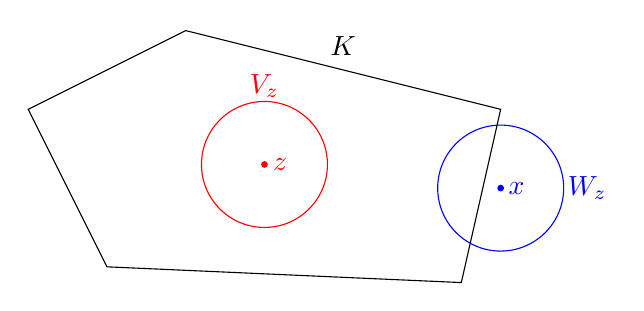
\begin{tikzpicture}
			\draw (-1,0) -- (-2,2) -- (0,3) -- (4,2) node[xshift=-2cm,yshift=8mm]{$K$} --
			(3.5,-0.2) --cycle;
			\draw[red] (1,1.3) node[yshift=1cm]{$V_z$} circle (0.8cm);
			\draw[red, fill=red] (1,1.3) node[xshift=2mm]{$z$} circle (1pt);
			\draw[blue] (4,1)node[xshift=1.1cm]{$W_z$} circle (0.8cm);
			\draw[blue, fill=blue] (4,1) node[xshift=2mm]{$x$} circle (1pt);
		\end{tikzpicture}
	\end{center}
	Now $\bigcup\limits_{z\in K}V_z\supset K$. So $\{V_z\}$ is an open cover of $K$.
	By compactness we have $V_{z_1}\cup V_{z_2}\cup \cdots\cup V_{z_n}\supset K$.
	As $W_z\cap V_z=\phi$ $\forall z\in K$.  We have $\underbrace{\left( W_{z_1}\cup
			W_{z_2}\cup \cdots \cup W_{z_n}\right) }_{\substack{\text{Finite intersection
				of}\\ \text{open neighborhoods of } x,\\ \text{so call this }U_x}}\cap K=\phi$
\end{myproof}

Key fact that made this work: For $x\neq z$ in $X$, we could find open neighborhoods of $V$ and $W$ (of $x$ and $z$ respectively) such that $V\cap W=\phi$. Topological spaces that satisfy this property are called \label{housdorff}Housdorff.

What we proved is the following
\begin{Theorem}{}{}
	For a Housdorff Topological space $X$ any compact subset $K$ is closed and bounded
\end{Theorem}

\begin{Theorem}{\hyperref[th:hnb]{Haine Borel Theorem} - If Part: \hyperref[hnb:st3]{Step \ref{hnb:st3}}}{hnb:s3}
	$C$ is a closed subset of compact set $X$ $\implies $ $C$ is compact.
\end{Theorem}
\begin{myproof}
	Take any open cover $\{V_{\alpha}\}_{\alpha\in I}$ of $C$ by open sets in $X$ i.e $\bigcup\limits_{\alpha}V_{\alpha}\supset C$. Now $\opensets \cup \{X\setminus C\}$ is an open cover of $x$. We have a finite subcover by compactness of $X$. The same subcover (after dropping $X\setminus C$ if necessary) works for $C$.
\end{myproof}
\wc{Closed interval $\bs{[a,b]}$ is compact in $\bs{\bbR}$}{Suppose $\opensets$ is an open cover of $[a,b]$ by open sets in $\bbR$.

Hence every one of the points in the interval is covered by one of the $V_{\alpha}$. Hence there is some interval contained in the $V_{\alpha}$
\begin{center}
	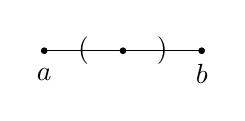
\begin{tikzpicture}
		\draw (-1,0) -- (1,0);
		\draw[fill=black] (-1,0) node[yshift=-3mm]{$a$} circle (1pt);
		\draw[fill=black] (1,0) node[yshift=-3mm]{$b$} circle (1pt);
		\draw (-0.5,0) node{$($};
		\draw (0.5,0) node{$)$};
		\draw[fill=black] (0,0) circle (1pt);
	\end{tikzpicture}
\end{center}
So i could just ignore the $V_{\alpha}$  and say for each point in the interval we can get an open interval that is part of a $V_{\alpha}$. So how can i find a subcover. I could simply travel from one end to the other.

So i start with $a$ so $a$ must be contained in some open interval
\begin{center}
	\begin{tikzpicture}
		\draw (-1,0) -- (1,0);
		\draw[red,fill=red] (-1,0) node[yshift=-3mm]{$a$} circle (1pt);
		\draw[fill=black] (1,0) node[yshift=-3mm]{$b$} circle (1pt);
		\draw[red] (-1.4,0) node{$($};
		\draw[red] (-0.6,0) node{$)$};
		\draw[<-,red] (-0.6,-0.2) -- (-0.6,-0.5) node[xshift=1mm,yshift=-2mm]{$\delta_1$};
	\end{tikzpicture}
\end{center}
Not only that i have covered up a small segment of the closed interval, upto a point, $a+\delta_1$. Say $[a,a+\delta_1)\subset V_1$.

Let $a+\delta_1$ is contained in some open interval which is contained in $V_2$ upto the point $a+\delta_2$
\begin{center}
	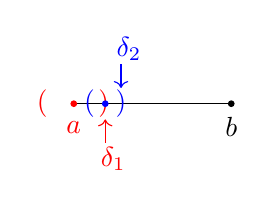
\begin{tikzpicture}
		\draw (-1,0) -- (1,0);
		\draw[red,,fill=red] (-1,0) node[yshift=-3mm]{$a$} circle (1pt);
		\draw[fill=black] (1,0) node[yshift=-3mm]{$b$} circle (1pt);
		\draw[red] (-1.4,0) node{$($};
		\draw[red] (-0.6,0) node[xshift=-0.2mm]{$)$};
		\draw[<-,red] (-0.6,-0.2) -- (-0.6,-0.5) node[xshift=1mm,yshift=-2mm]{$\delta_1$};
		\draw[blue] (-0.8,0) node{$($};
		\draw[blue] (-0.4,0) node{$)$};
		\draw[<-,blue] (-0.4,0.2) -- (-0.4,0.5) node[xshift=1mm,yshift=2mm]{$\delta_2$};
		\draw[blue,fill=blue] (-0.6,0) circle (1pt);
	\end{tikzpicture}
\end{center}
Now continue.
\tcbline\parinf
What is wrong with this ?\parinn

We could have smaller and smaller intervals. For example length of first interval can be $\frac13$, length of second interval can be $\frac19$, length of third interval can be $\frac1{27}$ and so on. So its a geometric progression and it will sum less than 1. So i just may not get there in finite number of steps.

}

\qs{}{Suppose $X$ is a topological space that is compact and \ref{housdorff} (Take $x$ ro be a compact metric space if you like). Prove that given disjoint compact subsets $K$ and $L$, there are disjoint open sets $U$ and $V$ with $K\subset U$ and $L\subset V$(First do it for $K=$ single point)}
In the above exercise we could have replaced the word compact with another word which is closed because $X$ is given to be compact so any closed set will be compact and in a Housdorff space compact subset is also closed.
\nt{Cauchy Sequence in Metric space need not converge. For example $(0,1)$ and take the sequence $\frac1n$. It wants to converge to 0 but 0 is not there.}


\begin{Theorem}{\hyperref[th:hnb]{Haine Borel Theorem} - If Part: \hyperref[hnb:st1]{Step \ref{hnb:st1}}}{hnb:s1}
	$[0,1]$ is compact in $\bbR$
\end{Theorem}
\begin{myproof}
	Let $\opensets$ be a family of open sets in $\bbR$ covering $[0,1]$.

	Let $S=\{a\in [0,1]\mid [0,a]\text{ can be covered by a finite number of }V_{\alpha}\text{'s}\}$. Our goal is to prove $1\in S$.

	Let $0\leq x<y\leq 1$. So $[0,x]\subset [0,y]$. This $y\in S\implies x\in S$ i.e $x\notin S\implies y\notin S$. Now $S$ is nonempty because $0\in S$ and $S$ is bounded. Let $u=\lub$ of $S$. Clearly $0\leq u\leq 1$. Hence it is enough to show $u=1$ and $u\in S$.

	$0\in$ some open set $V_{\alpha}$. Hence $\exists\ \eps>0$ $B_{\eps}(0)\subset \oset$. Hence $\forall$ point $x\in [0,\eps)$ $x\in S$

	For $a\in[0,u)$, $a\in S$ (otherwise $a$ itself would be an upper bound for $S$). As $\opensets$ cover $[0,1]$, $u\in V_{\beta}$. So $\exists \ \eps>0$ such that $(u-\eps,u+\eps)\subset V_{\beta}$ As $u-\eps\in S$ we have $\opset{1}\sup\opset{2}\sup\cdots\opset{k}\supset [0,u-\eps]$ Then $\opset{\beta}\cup\opset{1}\cup\opset{2}\cup \cdots\opset{k}\supset \left[0,u+\frac{\eps}{2}\right]$. So $u=1$ because otherwise some $u+\delta\in S$ contradicting that $u$ is an upper bound.
\end{myproof}
\qs{}{Can the strategy from the last time be made to work ti actually extract a finite subcover of a given cover.}
\begin{Theorem}{}{}
	Suppose $X\xrightarrow{f} Y$ continuous and $K\subset X$ is compact. Then $f(K)$ is compact
\end{Theorem}
\begin{myproof}
	Let $\opensets$ be an open cover of $f(k)$ by open sets $V_{\alpha}$ of $Y$. So $$\bigcup\limits_{\alpha}V_{\alpha} \supset f(K)\implies f^{-1}\left(\bigcup\limits_{\alpha}V_{\alpha}\right)=\bigcup\limits_{\alpha}f^{-1}\left(V_{\alpha}\right)\supset f^{-1}(f(K))\supset K$$ Thus $\left\{f^{-1}(V_{\alpha})\right\}_{\alpha\in I}$ is an open (because of continuity \hyperref[th:cont:invofopen]{Theorem \ref{th:cont:invofopen}}) cover of $K$.

	Extract a finite subcover \begin{align*}
		         & f^{-1}\left(V_{\alpha_1}\right)\cup f^{-1}\left(V_{\alpha_2}\right) \cup \cdots f^{-1}\left(V_{\alpha_m}\right)\supset K \\
		\implies & f\left(f^{-1}\left(V_{\alpha_2}\right) \cup \cdots f^{-1}\left(V_{\alpha_m}\right)\right)\supset f(K)                    \\
		\implies & \bigcup_{i=1}^m f\left(f^{-1}\left(V_{\alpha_i}\right)\right)\supset f(K)
	\end{align*}
	As $V_{\alpha_i}\supset f\left(f^{-1}\left(V_{\alpha_i}\right)\right)$ we have $\bigcup\limits_{i=1}^mV_{\alpha_i}\supset f(K)$
\end{myproof}
\qs{}{$f(\text{Sequentially compact }K)\text{ is sequentially compact}$}


\begin{Theorem}{\hyperref[th:hnb]{Haine Borel Theorem} - If Part: \hyperref[hnb:st2]{Step \ref{hnb:st2}}}{hnb:s2}
	$K=[a_1,b_1]\times[a_2,b_2]\times \cdots\times [a_n,b_n]$ is compact in $\bbR^n$
\end{Theorem}
\begin{myproof}
	Induction on $n$. $n=1$ we already proved in \hyperref[th:hnb:s1]{Theorem \ref{th:hnb:s1}}.Let $\mcF=\opensets$ be a cover of $K$ by open sets in $\bbR^n$. Fix $u\in [a_1,b_1]$ and consider  $\{u\}\times \underbrace{[a_2,b_2]\times \cdots\times [a_n,b_n]}_{\substack{=C\text{ is compact}\\\text{by induction on }n}}$ Hence $\{u\}\times C$ is compact because   $\bbR^{n-1}\to\bbR^n$ which maps $(y_2,y\cdots,y_n)\mapsto (u,y_2,\cdots,y_n)$ or $ {f(C)=\{u\}\times C} $ is continuous.

	For each $p=(u,y_2,\cdots,y_n)$ in $\{u\}\times C$ pick an open neighborhood $V_p\in \mcF$. Hence $V_{p}\supset (x-\eps,x+\eps)\times \underbrace{(y_2-\eps,y_2+\eps)\times \cdots\times (y_n-\eps,y_n+\eps)}_{W_p}$ for some $\eps=\eps_p$ depending on $p$
	\begin{center}
		\begin{tikzpicture}
			\draw (0.5,5)node[yshift=-5.3cm]{$a_1$} rectangle (6,0)node[yshift=-0.3cm]{$b_1$};
			\draw (3,0) node[yshift=-0.3cm]{$u$} -- (3,5);
			\draw[blue] (2.5,0) rectangle (3.5,5);
			\draw[red] (1.5,0) rectangle (4.5,3);
			\draw[red,fill=red] (3,1.5) circle (1pt);
			\draw[red] (2.3,2.5) rectangle (3.7,3.9);
			\draw[red,fill=red] (3,3.2) circle (1pt);
			\draw[red]  (2.2,5) rectangle (3.8,3.4);
			\draw[red,fill=red] (3,4.2) circle (1pt);
		\end{tikzpicture}
	\end{center}
	By compactness of $\{u\}\times C$, extract a finite subcover of the cover $\{W_p\}$. Hence $W_{p_1}\cup W_{p_2}\cup\times \cup W_{p_k}\supset \{u\}\times C$. Since its a union of open sets we have in fact $W_{p_1}\cup W_{p_2}\cup\times \cup W_{p_k}\supset (u-\eps,u+\eps)\times C$ where $\eps=\min\{\eps_{p_1},\eps_{p_2},\cdots,\eps_{p_k}\}$. Let $\mcF_u=\{V_{p_1},V_{p_2}<\cdots,V_{p_k}\}$. So $$V_{p_1}\cup V_{p_2}\cup \cdots\cup V_{p_k}\supset W_{p_1}\cup W_{p_2}\cup\cdots\cup W_{p_k}\supset (u-\eps,u+\eps)\times C$$i.e. this finite subcover $\mcF_u$ cover not just the slice but a tube around it.

	Now as $u$ varies in $[a_1,b_1]$, $(u-\eps_u,u+\eps_u)$ gives an open cover. Extract a finite subcover  $(u_1-\eps_{u_1},u_1+\eps_{u_1}),(u_2-\eps_{u_2},u_2+\eps_{u_2}),\cdots,(u_l+\eps_{u_l},u_l+\eps_{u_l})$ . Then $\mcF_{u_1}\cup\mcF_{u_2}\cup\cdots\cup\mcF_{u_l}$ is a finite subcover of $[a_1,b_1]\times C=K$
\end{myproof}
\qs{}{Why the map $\bbR^{n-1}\to\bbR^n$ which maps $(y_2,y\cdots,y_n)\mapsto (u,y_2,\cdots,y_n)$ or $ {f(C)=\{u\}\times C} $ is continuous ?}
\qs{}{$X,Y$ are topological spaces. $K\subset X$ and $Y\subset Y$ are compact subsets. Then $K\times L$ is compact subset of $X\times Y$ where Open sets of $X\times Y$ are $\bigcup$(Open set of $X$)$\times$(Open set in $Y$)}

\begin{Theorem}{}{all norms equiv}
	All norms on $\bbR^n$ are equivalent
\end{Theorem}
\begin{myproof}
	Enough to show any norm $f \sim \norm$  \begin{align*}
		 & \text{i.e }\alpha \|u\|\leq f(u)\leq \beta\|u\| \forall\ u                        \\
		 & \text{i.e } \alpha \leq \frac{f(u)}{\|u\|}\leq \beta\ \forall\ u \forall\ u\neq 0
	\end{align*}
	Note that $\frac{f(x)}{\|x\|}=f\left(\frac{x}{\|x\|}\right)=f(u)$ where $u=\frac{x}{\|x\|}$, so $\|u\|=1$. Hence it is enough to show that $$\alpha\leq f(u)\leq \beta$$for any $u$ with $\|u\|=1$

	Let $S=\{u\mid \|u\|=1\}$ is the unit sphere in $\bbR^n$, which is closed and bounded

	\begin{center}
		\begin{tabular}{rcl}
			$S$ is closed and bounded & $\implies$ & $S$ is compact                                        \\
			                          & $\implies$ & $f(S)$ is compact in $\bbR$                           \\
			                          & $\implies$ & $f(S)$ is closed and bounded in $\bbR$                \\
			                          & $\implies$ & $f(S)$ has largest element in $\beta$ and smallest    \\
			                          &            & element $\alpha$ such that $\alpha\leq f(S)\leq\beta$
		\end{tabular}
	\end{center}
\end{myproof}




\chapter{Differentiation }
Derivative of $f$ at $a\in \bbR$ is $$f'(a)=\lim_{h\to 0} \frac{f(a+h)-f(a)}{h}$$To take this limit $f$ should be defined in some $(a-\eps,a+\eps)$ i.e. $f:\text{ neighborhood of }a\to\bbR$\parinf

\textbf{Goal:} Definition of $f'(a)$ for $a\in $(Some open $U$ in $\bbR^m$)$\xrightarrow{f}\bbR^n$, $a,h\in\bbR^m$\parinn

$f(a+h)-f(a)$ makes sense in $\bbR^n$ but can't divide by $h$, which is a vector in $\bbR^m$. If $m=1$ can use the same definition. ${f:\text{ Open }U\text{ in a }\bbR\to\bbR^n}$ which maps $a\mapsto(f_1(a),f_2(a),\cdots,f_n(a))$. If $n=1$ i.e. $\bbR^m\supset U\xrightarrow{f}\bbR$  we have partial derivatives.
\ex{Derivative of $f:\bbR^m\to\bbR$}{$f(x,y,z)=x^4\sin (yz)$. Here\begin{align*}
		\del{f}{x} & =4x^3\sin(yz)                               \\
		           & =\lim_{h\to 0}\frac{f(x+h,y,z)-f(x,y,z)}{h}
	\end{align*}Hence 	\begin{align*}
		\left.\del{f}{x}\right|_{p=(r,s,t)} & =\lim_{h\to 0}\frac{f(r+h,s,t)-f(r,s,t)}{h}                                                            \\
		                                    & =\lim_{h\to 0}\frac{f(p+he_1)-f(p)}{h}\qquad[p=re_1+se_2+te_3\text{ using standard basis }e_1,e_2,e_3]
	\end{align*} Its a real number if the limit exists
}
\section{Partial Derivatives}
\dfn{Partial Derivative  of $\bs{f:\bbR^n\supset U\to \bbR}$}{For $f: $(Open $U$ in $\bbR^m$)$\to\bbR^n$, define ``$i-$th partial derivative of $f$ at $a\in U$" to be $\left(\text{Notation }\left.\del{f}{x_i}\right|_a,\right.$ $\left.\del{f}{x_i}(a),D_if(a)\right)$ $\lim\limits_{h\to a}\frac{f(a+he_i)-f(a)}{h}\qquad(i=1,2,\cdots,m)$}

Note that this limit (if exists) is in $\bbR^n$. $$\begin{rcases*}
		\text{If }f=(f_1,f_2,\cdots,f_n)\ (f_i\text{ real} \\ \text{values in function }U\to\bbR)
	\end{rcases*}\del{f}{x_i}(a)=\left(\del{f_1}{x_i}(a),\del{f_2}{x_i}(a),\cdots,\del{f_n}{x_i}(a)\right)$$So for $f:U\to \bbR^m$, $a\in U$ we get $\del{f_j}{x_i}$ where $1\leq j\leq n$ and $1\leq i\leq m$. We can arrange these  in a  matrix  of dimensions $n\times m$ $$\begin{bmatrix}
		\deld{f_1}{x_1}(a) & \cdots & \deld{f_1}{x_m}(a) \\
		\vdots             & \ddots & \vdots             \\
		\deld{f_n}{x_1}(a) & \cdots & \deld{f_n}{x_m}(a)
	\end{bmatrix}$$\nt{$f'(a)$ can be defined as a linear map $\bbR^n\to\bbR^m$

	In the old situation $f:\bbR\to\bbR$, $f'(a)\in\bbR$ is a $1\times 1$ matrix, as such it encodes a linear map $\underset{x\mapsto f'(a)x}{\bbR\to\bbR}$
	\begin{center}
		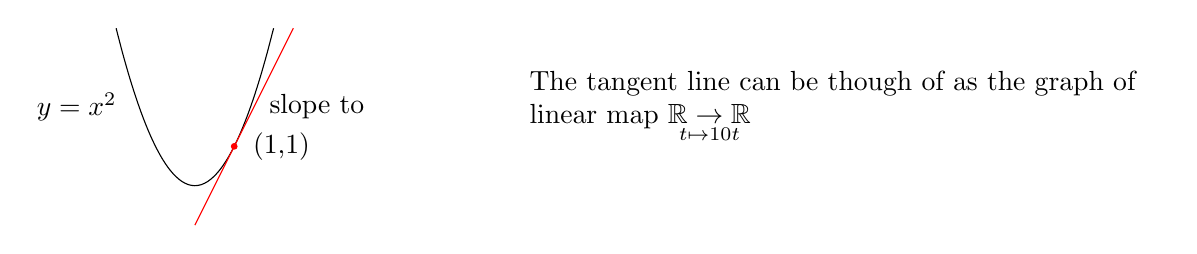
\begin{tikzpicture}
			\draw[scale=0.5,domain=-2:2, smooth, variable=\x] plot ({\x}, {\x*\x});
			\draw (0,0) node[xshift=-1.5cm,yshift=1cm]{$y=x^2$};
			\draw[scale=0.5,red,fill=red] (1,1) circle (2pt);
			\draw[scale=0.5,red] (2.5,4) node[xshift=3mm,yshift=-1cm,color=black]{slope to} -- (0,-1);
			\draw[scale=0.5] (1,1) node[xshift=6mm]{(1,1)};
			\draw[scale=0.5] (2.5,4) node[xshift=7cm,yshift=-1cm,text width=8cm]{The tangent line can be though of as the graph of linear map $\underset{t\mapsto 10t}{\bbR\to\bbR}$};
		\end{tikzpicture}
	\end{center}
}
\section{Differentiation}
$f'(a)$ is a number such that $\lim\limits_{h\to 0}\frac{f(a+h)-f(a)-f'(a)h}{h}=0$. Inspired by this for $a\in U (\text{Open in }\bbR^m)\xrightarrow{f}\bbR^n$, we define $f'(a)$ is a linear map $\bbR^m\to\bbR^n$ such that $$\lim\limits_{h\to 0}\frac{\|f(a+h)-f(a)-f'(a)h\|}{\|h\|}=0\text{ in }\bbR $$($h$ is a small vector $\in\bbR$)
\dfn{Differentiation of $\bs{f:\bbR^m\supset U\to \bbR^n}$}{$U$ open set in $\bbR^m$, $f:U\to\bbR^n$, $a\in U$ given. We say that $f$ is differentiable  at $a$  if there is a  linear map  $T:\bbR^m\to\bbR^n$ such that $$\lim_{h\to 0}\frac{\|f(a+h)-f(a)-T(h)\|}{\|h\|}=0$$i.e $\forall\ \eps>0$, $\exists\ \delta>0$ s.t. $$\|h\|<\delta\implies \dfrac{\|f(a+h)-f(a)-T(h)\|}{\|h\|}<\eps$$We call such a linear map $T$ the derivative  of $f$ at $a$, denoted by $f'(a),D(f(a))$}
Note that $f'(a)h$ = Value of linear map $f'(a)$ applied to a vector $h$
\nt{If the above limit is 0 w.r.t any norm on $\bbR^M$ (respectively $\bbR^n$) then the same limit is 0 w.r.t any other norm on $\bbR^m$ (respectively $\bbR^n$) because \hyperref[th:all norms equiv]{all norms are equivalent}}
\begin{Theorem}{}{}
	Derivative is unique i.e. if $a\in U (\text{Open in }\bbR^m)\xrightarrow{f}\bbR^n$,  and $$\lim_{h\to 0}\frac{\|f(a+h)-f(a)-T(h)\|}{\|h\|}=0 =\lim_{h\to 0}\frac{\|f(a+h)-f(a)-S(h)\|}{\|h\|}$$then $T=S$ i.e $T(v)=S(v)$ $\forall\ v\in\bbR^m$
\end{Theorem}
\begin{myproof}
	Let $R=S-T$. Want to show $R(v)=0$ $\forall \ v\in\bbR^m$ \begin{multline*}
		\frac{\|R(h)\|}{\|h\|}=\frac{\|S(h)-T(h)\|}{\|h\|}=\frac{\|(f(a+h)-f(a)-T(h))-(f(a+h)-f(a)-S(h))\|}{\|h\|} \\
		\leq \frac{\|(f(a+h)-f(a)-T(h))\|}{\|h\|}+\frac{\|(f(a+h)-f(a)-S(h))\|}{\|h\|}
	\end{multline*}Taking $\lim\limits_{h\to 0}$, we get $\lim\limits_{h\to 0}\frac{\|R(h))\|}{\|h\|}=0$.

	Fix any nonzero $v$, $\lim\limits_{\lm\to 0}\lm v=0$. Take $h=\lm v$ ($\lm\neq 0$)$$\frac{\|R(h)\|}{\|h\|}=\frac{|\lm|\|R(v)\|}{|\lm|\|v\|}=\frac{\|R(v)\|}{\|v\|}$$Hence $$0=\lim\limits_{h\to 0}\frac{\|R(h)\|}{\|h\|}=\lim_{h\to 0}\frac{\|R(v)\|}{\|v\|}\implies\|R(v)\|=0\implies Rv=0$$
\end{myproof}
\qs{}{If $f:\underset{v\mapsto Av}{\bbR^m\to\bbR^n}$ is a linear map then what is $f':\bbR^m\to\bbR^n$}
\sol{See that $f'(a)=f$. (Immediate from definition)\Qed}
\qs{}{For an affine map $\underset{v\mapsto Av+c}{\bbR^m\xrightarrow{g}\bbR^n}$ for some $c\in\bbR^n$. Calculate $g'(a)$.}
\sol{$g'(a)=$ the map $h\mapsto Ah$\Qed}
\begin{Theorem}{Matrix of $f'(a)$}{}
	Prove that the matrix  of $f'(a)$ w.r.t standard basis of $\bbR^m$ and $\bbR^n$ is the Jacobian Matrix
\end{Theorem}
\begin{myproof}
	$j$th column of matrix of $T=T(e_j)\in\bbR^n$
	\begin{align*}
		  & \lim_{\lm\to0}\frac{\|f(a+\lm e_j)-f(a)-T(\lm e_j)\|}{\|\lm e_j\|}\text{ by definition of }T=f'(a)    \\
		= & \lim_{\lm\to0}\frac{\|f(a+\lm e_j)-f(a)-\lm T(e_j)\|}{|\lm|}\begin{cases*}
			                                                                T(\lm e_j)=\lm T(e_j)\text{ by linearity} \\
			                                                                \|\lm e_j\|=|\lm|\|e_j\|=|\lm|
		                                                                \end{cases*} \\
		= & \lim_{\lm\to0}\left\|\frac{f(a+\lm e_j)-f(a)}{|\lm|}-\frac{\lm T(e_j)}{|\lm|}\right\|
	\end{align*}Hence for $\lm>0$ $$\lim_{\lm\to0}\frac{f(a+\lm e_j)-f(a)}{|\lm|}-T(e_j)=0$$Let $f=\begin{bmatrix}
			f_1\\ f_2 \\ \vdots\\ f_n\end{bmatrix}$. Hence \begin{align*}
		T(e_j) & =\lim_{\lm\to 0}\frac{f(a+\lm e_j)-f(a)}{\lm}                                      \\
		       & =\lim_{\lm\to 0}\frac{\begin{bmatrix}
				                               f_1(a+\lm e_j) \\
				                               f_2(a+\lm e_j) \\
				                               \vdots         \\
				                               f_n(a+\lm e_j)
			                               \end{bmatrix}-\begin{bmatrix}
				                                             f_1(a) \\
				                                             f_2(a) \\
				                                             \vdots \\
				                                             f_n(a)
			                                             \end{bmatrix}}{\lm} =\begin{bmatrix}
			                                                                  \deld{f_1}{x_j}(a) \\[5mm]
			                                                                  \deld{f_2}{x_j}(a) \\[3mm]
			                                                                  \vdots             \\
			                                                                  \deld{f_n}{x_j}(a)
		                                                                  \end{bmatrix}
	\end{align*}Matrix of $f'(a)$= Jacobian Matrix $$\begin{bmatrix}
			\deld{f_1}{x_1}(a) & \cdots & \deld{f_1}{x_m}(a) \\
			\vdots             & \ddots & \vdots             \\
			\deld{f_n}{x_1}(a) & \cdots & \deld{f_n}{x_m}(a)
		\end{bmatrix}$$We have proved if $f'(a)$ exists, then  all partial derivatives  $\del{f_i}{x_j}$ exists at $x=a$ and make up the matrix  of $f'(a)$
\end{myproof}
If all $\del{f_i}{x_j}$ exists at $x=a$, does not imply  $f$ is differentiable at $x=a$?
\qs{}{Under Which conditions if all $\del{f_i}{x_j}$ exists at $x=a$, it implies that $f$ is differentiable at $x=a$?}
\begin{Theorem}{}{}
	If $f'(a)$ exists then $f$ is continuous at $x=a$
\end{Theorem}
\begin{myproof}
	If $f'(a)$ exists then $f$ is continuous at $x=a\iff\lim\limits_{h\to 0}f(a+h)=f(a)\iff\lim\limits_{h\to 0}\|f(a+h)-f(a)\|=0$
	$$\|f(a+h)-f(a)+T(h)-T(h)\|\leq \|f(a+h)-f(a)-T(h)\|+\|T(h)\|$$Now $\lim\limits_{h\to 0}\dfrac{\|f(a+h)-f(a)-T(h)\|}{\|h\|}\|h\|=0\cdot 0=0$ and $$\lim_{h\to 0}\|T(h)\|=0\text{ because }\begin{cases*}
			T\text{ is continuous (being linear) so} \\
			T(h)\to T(0)=0
		\end{cases*}$$
\end{myproof}


\chapter{Examples on Multivariable Differentiation}
\begin{example}{Example where all partial derivatives exist and function is continuous but $f'$ does not exists.}{}
		$f(x,y)=\begin{cases}
		\frac{xy}{\sqrt{x^2+y^2}}& (x,y)\neq (0,0)\\
		0 & (x,y)=(0,0)
	\end{cases}$
\begin{enumerate}[label=(\roman*)]
	\item Is $f$ continuous at origin ?
	\item Do $\deld{f}{x}, \deld{f}{y}$ exist at origin ? elsewhere ?
\end{enumerate}
\end{example}
\sol{
\begin{enumerate}[label=(\roman*)]
	\item Want $|f(x,y)-f(0,0)|\to 0$ as $(x,y)\to (0,0)$ $$\lt| \frac{xy}{\sqrt{x^2+y^2}}\rt|\leq \sqrt{\frac{x^2+y^2}{2}}\to 0$$as $(x,y)\to (0,0)$
	\item $$\del{f}{x}=\frac{y^3}{(x^2+y^2)^{\frac{3}{2}}}\qquad \del{f}{y}=\frac{x^3}{(x^2+y^2)^{\frac{3}{2}}}$$Now $$\lt.\del{f}{x}\rt|_{(0,0)}=\lim_{h\to 0}\frac{f(h,0)-f(0,0)}{h}=\lim_{h\to 0}\frac{0-0}{h}=0$$Similarly $\lt.\del{f}{y}\rt|_{(0,0)}=0$. So if $f'(0)$ exists then  it will be the matrix $\lt[\begin{matrix}0 & 0\end{matrix} \rt]$. So it will be the zero operator $\implies D_vf(\text{origin})=0$ for any direction  for any vector $v$. Let's test for $v=\lt[\begin{matrix}1 \\ 1\end{matrix} \rt]$ $$D_vf(\text{origin})=\lim_{t\to 0}\frac{f(0+tv)-f(0,0)}{t}=\lim_{t\to 0}\frac{f(t,t)}{t}=\lim_{t\to 0}\frac{t^2}{t\sqrt{2t^2}}\neq 0$$Thus $f$ is not differentiable at origin. Therefore at least one of the partial derivatives must be discontinuous at origin (here by symmetry both are discontinuous). $\del{f}{x}=0$ at origin but $=1$ at $y-$axis.
\end{enumerate}
}
\begin{example}{Example where $f'$ exists but not continuous}{}
	Recall one-variable example $g(x)=\begin{cases}
		x^2\sin \frac1x & x\neq 0\\ 0 & x=0
	\end{cases}$. Define $f(x,y)=g(\sqrt{x^2+y^2})$
\begin{enumerate}[label=(\roman*)]
	\item Is $f$ continuous ?
	\item Is $f$ differentiable ?
	\item Is $f'$ continuous at origin ?
\end{enumerate}
\end{example}
\sol{
\begin{enumerate}[label=(\roman*)]
	\item Because $f$ is composition of two continuous functions. $f$ is continuous.
	\item Need to check at origin only
\end{enumerate}
}
\begin{example}{}{}
	$f(x,y)=\begin{cases}
		\frac{x^2y}{x^6+y^2}& (x,y)\neq (0,0)\\
		0 & (x,y)=(0,0)
	\end{cases}$
\begin{enumerate}[label=(\roman*)]
	\item Is $f$ continuous at origin ?
	\item Calculate the directional derivatives for unit vectors $u=(\cos\theta,\sin\theta)$
	\item Is $f$ differentiable at origin ?
\end{enumerate}
\end{example}
\sol{
	\begin{enumerate}[label=(\roman*)]
		\item $$f(x,x^3)=\frac{x^5}{2x^6}=\frac{1}{2x}$$It has no limit  as $x\to 0$. Hence $f$ is not continuous at origin. 
		\item \begin{align*}
			D_uf(0) & =\lim_{h\to 0}\frac{f(0+hu)-f(0)}{h}\\
			& =\lim_{h\to 0} \frac{f(h\cos\theta,h\sin\theta)}{h}\\
			&=\lim_{h\to 0} \frac1h \frac{h^3\cos^2\theta \sin\theta}{h^6\cos^6\theta+h^2\sin^2\theta}\\
			&=\lim_{h\to 0} \frac{\cos^4\theta\sin\theta}{h^4\cos^6\theta+\sin^2\sin\theta}=\frac{\cos^2\theta}{\sin\theta}\qquad\text{when }\sin\theta\neq 0
		\end{align*}When $\sin\theta=0$, $f=0$ on $x-$axis. So $D_uf(0)=0$ for $\theta=0,\pi,\dots$. SO $D_uf()$ exists for all $u$
	\item If $f'(0)$ exists then it's matrix would be $\lt[ \begin{matrix} & 0\end{matrix} \rt]$. But then all directional  derivatives would have to be zero because $D_uf(a)=f'(a)v$ which is not possible 
	\end{enumerate}
}

\chapter{Chain Rule of Differentiation and Operator Norm}
\section{Operator Name}
$V,W$ are vector spaces. $\mcL(V,W)=$ Set of linear maps $V\to W$ is a vector space via $(A+B)(v)=A(v)+B(v)$ and $A(\lm v)=\lm A(v)$

If $V=\bbR^m$ and $\bbR^n$, $\dim (\bbR^m,\bbR^n)=mn$. We can identity $\mcL(\bbR^m,\bbR^n)$ with $n\times m$ matrices. $$\|A\|_{\mcL(\bbR^m,\bbR^n)}=\|A\|=\sup\limits_{\|u\|=1} \|A(u)\|$$This gives a norm because $\|A\|\geq 0$ and $\|A\|=0\implies A=0$ and  $\|\lm A\|=|\lm|\|A\|$. As  $(A+B)(u)=A(u)+B(u)$ we have $\|(A+B)(u)\|\leq \\A(u)\|+\|B(u)\|$ in $W$ and hemce $\|A+B\|\leq \|A\|+\|B\|$.
\qs{}{Why this is well defined ?}
\solve{The set $S=\{u\mid \|u\|=1\} $ is closed and bounded in $V$, therefore compact. $A$ being linear  is continuous. $\therefore A(S)$ is a compact subset of $W\implies A(S)$ is bounded.}

\textbf{Basic Properties:-}
\begin{enumerate}
	\item $\|Av\|\leq \|A\| \|v\|$ i.e. $\|Av\|_W\leq \|A\|_{\mcL}\|v\|_V$
	      \begin{myproof}
		      If $v=0$ then we are done. If $v\neq 0$, $u=\frac{v}{\|v\|}$ so $\|u\|=1$. Hence $$\|A\|\geq \|Au\|=\left\|A\left(\frac{v}{\|v\|}\right)\right\|=\frac{\|Av\|}{\|v\|}$$
	      \end{myproof}
	\item $\|A(v)\|\leq M\|v\|$ for all $v\implies \|A\|\leq M$ in fact $\inf\{M\mid \|A(v)\|\leq M\|v\|\ \forall\ v\}$
	      \begin{myproof}
		      Suppose $\|A(v)\|\leq M\|v\|$ $\forall\ v$. In particular $\forall\ v$ with $\|v\|=1$. So $\|A(v)\|\leq M$.

		      Rest exercise: If $L<\inf$ of the set  show $\exists \ u$ of norm=1 with $\|A(v)\| >L$.
	      \end{myproof}
	\item $U\xrightarrow{A}V\xrightarrow{B}W$ linear maps between finite dimensional vector spaces  then $\|BA\|\leq \|B\|\|A\|$
	      \begin{myproof}
		      Take $u$ with $\|u\|=1$. Then $$\|BA(u)\|\leq \|B\|\|A(u)\|\leq \|B\|\|A\|\|u\|=\|B\|\|A\|$$Now take $\sup$ over $u$.
	      \end{myproof}
	      \nt{$\underset{\mcL(U,V)\oplus\mcL(V,W)}{A,B}\underset{\to}{\mapsto}\underset{\mcL(U,W)}{BA}$ is continuous because  each slot of matrix of $BA$ is obtained by adding/multiplying entries of $A$ and $B$.}
\end{enumerate}
\qs{}{Show $A_n\to A$ in $\mcL(U,V)$, $B_n\to B$ in $\mcL(V,W)$ then $B_nA_n\to BA$ in $\mcL(U,W)$}

\section{Chain Rule}

\begin{Theorem}{}{}
	Let\begin{center}
		\begin{tikzcd}[ampersand replacement = \&]
			\&[-1cm]       \&\mathbb{R}^n     \&              \\[-0.7cm]
			\&[-1cm]          \& \usubset          \&              \\[-0.7cm]
			\mathbb{R}^m \supset \&[-1cm] U \arrow[r, "f"]     \& V \arrow[r, "g"] \& \mathbb{R}^k \\[-0.7cm]
			\&[-1cm] \uin                  \& \uin              \&              \\[-0.7cm]
			\&[-1cm] a \arrow[r, maps to] \& b                \&
		\end{tikzcd}
	\end{center} $f$ is differentiable at $a$. and $g$  is differentiable at $b=f(a)$. Then $g\circ f$ is differentiable at $a$  and $$(g\circ f)'(a)=\underbrace{g'(f(a))f'(a)}_{\substack{\text{Multiplication}\\ \text{of matrices}}}$$
\end{Theorem}
\begin{myproof}
	\subsubsection{1-Variable Case}
	$\frac{dz}{dx}=\frac{dz}{dy}\, \frac{dy}{dx}$\begin{align*}
		\frac{dz}{dx} =\lim_{\Delta x\to 0} \frac{\Delta z}{\Delta x} & =\lim_{\Delta x\to 0}\frac{\Delta z}{\Delta y}\, \frac{\Delta y}{\Delta x}                                                                  \\
		                                                              & =\lim_{\Delta x\to 0}\frac{\Delta z}{\Delta y}\lim_{\Delta x\to 0} \frac{\Delta y}{\Delta x}                                                \\
		                                                              & =\lim_{\Delta y\to 0}\frac{\Delta z}{\Delta y}\lim_{\Delta x\to 0} \frac{\Delta y}{\Delta x}\qquad [\text{As }\Delta x\to0,\ \Delta y\to 0]
	\end{align*}
	\subsubsection{Multi Variable Case}
	Note that $\bbR^m\xrightarrow{f'(a)}\bbR^n\xrightarrow{g'(f(a))}\bbR^k$

	If $T=f'(a)$ then $$\lim_{h\to 0}\frac{\|f(a+h)-f(a)-T(h)\|}{\|h\|}=0$$and $S=g'(f(a))=g'(b)$ then $$ \lim_{h\to 0}\frac{\|g(b+k)-g(b)-S(k)\|}{\|k\|}=0$$Let \begin{align*}
		\alpha(h) & = f(a+h)-f(a)-T(h) & \eps(h) & = \frac{\|\alpha(h)\|}{\|h\|}\to 0\text{ as }h\to 0  \\[3mm]
		\beta(k)  & = g(b+k)-g(b)-S(k) & \eta(k) & = \begin{cases*}
			                                             \dfrac{\|\beta(k)\|}{\|k\|}\to0  \text{ as }k\to 0 \\
			                                             0      \text{ when }                         k=0
		                                             \end{cases*}
	\end{align*}
	$\eta$ is continuous at $k=0$. Now note that $\eta:V-b\to \bbR$ because we ae always taking $b+k$ for $\eta$. We want to show that \[\lim_{h\to 0}\frac{\|g(f(a+h))-g(f(a))-ST(h)\|}{\|h\|}=0\iff \lim_{k\to 0}\frac{\|g(b+k)-g(b)-ST(h)\|}{\|h\|}=0\]where $f(a+h)=b+k\iff k=f(a+h)-f(a)$. We have taken a specific value of $k$ depending on $h$. So now $k$ is a function of $h$. Hence $T(h)=f(a+h)-f(a)-\alpha(h)=k-\alpha(h)$
	\begin{align*}
		  & g(b+k) -g(b) -ST(h)           \\
		= & g(b+k) -g(b) -S(k-\alpha(h))  \\
		= & g(b+k)-g(b)-S(k)+S(\alpha(h))
	\end{align*}Therefore\[ \frac{\|g(b+k)-g(b)-ST(h)\|}{\|h\|}\leq \frac{\|g(b+k)-g(b)-S(k)\|}{\|h\|}+\frac{\|S(\alpha(h))\|}{\|h\|}\] want to bound each of these separately
	\[\frac{\|S(\alpha(h))\|}{\|h\|}\leq \|S\|\frac{\|\alpha(h)\|}{\|h\|}\to 0\]Now how to bound the first term. In the first term $\frac{\|\beta(k)\|}{\|h\|}=\eta(k)\frac{\|k\|}{\|h\|}$. Now \begin{align*}
		         & k=T(h)+\alpha(h)                                                                                                                                                        \\
		\implies & \|k\|\leq \|T(h)\|+\|\alpha(h)\|                                                                                                                                        \\
		\implies & \frac{\|k\|}{\|h\|}\leq \frac{\|T(h)\|}{\|h\|}+\frac{\|\alpha(h)\|}{\|h\|}\leq \frac{\|T\|\|h\|}{\|h\|}+\frac{\|\alpha(h)\|}{\|h\|} = \|T\|+\frac{\|\alpha(h)\|}{\|h\|}
	\end{align*}Hence $$\frac{\|\beta(k)\|}{\|k\|}=\eta(k)\frac{\|k\|}{\|h\|}\leq \eta(k)\lt[\|T\|+\frac{\|\alpha(h)\|}{\|h\|}\rt]$$As $h\to 0$ $\|T\|+\frac{\|\alpha(h)\|}{\|h\|}\to \|T\|+0$ which is finite. And as $h\to 0$, $k\to 0\implies \eta(k)\to 0$ because $\eta$ is continuous at 0.
\end{myproof}

\section{Special Case of Chain Rule: When \texorpdfstring{$m=k=1$}{m=k=1}}
Open interval in $\bbR\xrightarrow{\gamma}\bbR^n\xrightarrow{g}\bbR$. $\gamma=$ parameterized curve in $\bbR^n$
$$(g\circ \gamma)'(t)=g'(\gamma(t))\cdot \gamma'(t)$$ ${\bbR\xrightarrow{\gamma}\bbR^n}$ maps $t\to\begin{bmatrix}\gamma_1(t)\\ \vdots\\ \gamma_n(t)	\end{bmatrix}$ hence $\gamma'(t)=\begin{bmatrix}
		\gamma_1'(t) \\ \vdots\\ \gamma_n'(t)
	\end{bmatrix}$

Now $g'(y)=\begin{bmatrix}
		\lt.\deld{g}{x_1}\rt|_y\cdots \lt.\deld{g}{x_n}\rt|_y
	\end{bmatrix}$. Hence \begin{align*}
	(g\circ \gamma)'(t) & = \begin{bmatrix}
		                        \lt.\deld{g}{x_1}\rt|_y\cdots \lt.\deld{g}{x_n}\rt|_y
	                        \end{bmatrix}\begin{bmatrix}
		                                     \gamma_1'(t) \\ \vdots\\ \gamma_n'(t)
	                                     \end{bmatrix}                                  \\
	                    & = \begin{bmatrix}
		                        \lt.\deld{g}{x_1}\rt|_y \\ \vdots \\ \lt.\deld{g}{x_n}\rt|_y
	                        \end{bmatrix}\cdot \begin{bmatrix}
		                                           \gamma_1'(t) \\ \vdots\\ \gamma_n'(t)
	                                           \end{bmatrix}\qquad[\text{Usual dot product of vectors in }\bbR^n] \\
\end{align*}
\pagebreak

Call $\begin{bmatrix}
		\lt.\del{g}{x_1}\rt|_y \\ \vdots \\ \lt.\del{g}{x_n}\rt|_y
	\end{bmatrix}$ = $\nabla g(\gamma(t))=$ Gradient of $g$ at the point $\gamma(t)$. Hence $(g\circ\gamma)'(t)=\nabla g(\gamma(t))\cdot\gamma'(t)$
\qs{}{Fix $u,v\in \bbR^n$ and take parametrized curve $\gamma(t)=u+tv$. What does the above equation give at $t=0$ (for a given function $g$)}




\chapter{Mean Value Theorem}
We will use Euclidean norm on $\bbR^n$ and have Cauchy-Schwarz Inequality $|v\cdot w|\leq \|v\|\|w\|$.
\begin{theorem}{1-Variable MVT}{1varmvt}
	If $f:[a,b]\to \bbR$ continuous and $f'$ exists on $(a,b)$, then $\exists\ c\in(a,b)$ s.t $$f(a)-f(b)=f'(c)(b-a)$$
\end{theorem}
\begin{myproof}1-variable MVT

	\hspace{1cm} $\Uparrow$ Via Rolle's Theorem, using $f'(\text{extremum})=0$

	\hspace*{0.5cm}Extreme Value Theorem

	\hspace{1cm} $\Uparrow$ $[a,b]$ is compact, $f$ is continuous $\implies f([a,b])$ is compact in $\bbR\implies $ closed and bounded

	\hspace*{0.5cm}Heine Borel Theorem
\end{myproof}

\qs{}{First consider $f:[a,b]\to\bbR^n$ continuous and $f'$ exists on $(a,b)$. Is there a $c\in (a,b)$ s.t. $$\|f(b)-f(a)\|\overset{?}{=}\|f'(c)\|(b-a)$$}
\solve{No. For example $f:[0,2\pi]\to\bbR^2$ which maps $t\mapsto (\sin t,\cos t)$. Then $f'(t)=(\cos t,-\sin t)$ and $\|f'(t)\|=1$. $f(2\pi)-f(0)=(0,0)$}
\begin{theorem}{MVT of Real-Valued Functions}{}
	Let $f$ be a continuous function $[a,b]\to \bbR^n$ and $f'(c)$ exists $\forall\ c\in(a,b)$. Then $\exs\ c\in (a,b)$ s.t $$\|f(b)-f(a)\|\leq (b-a)\|f'(c)\|$$(Here the norm is Euclidean norm. For the inequality which norm we take does matter.)
\end{theorem}
\begin{myproof}
	Clever use if \hyperref[th:1varmvt]{$1-$Variable MVT}. We want to bound norm of $f(b)-f(a)=z$.\parinf

	\textbf{Idea: }Dot with $z$ and then use Cauchy Schwarz \parinn
	\begin{center}
		\begin{tikzcd}
			{[a,b]} \arrow[r, "f"]                                     & \mathbb{R}^n \arrow[r, "{g=\langle -,z\rangle}"] & \mathbb{R}              \\[-0.7cm]
			t \arrow[r, maps to] \arrow[rr, "\phi(t)"', bend right=49] & f(t) \arrow[r, maps to]                        & {\langle f(t),z\rangle}
		\end{tikzcd}
	\end{center}
	Notice $g: \bbR^n\to\bbR$ where $g$ maps $x\longmapsto \langle x,z\rangle=x_1z_1+\cdots+x_nz_n$. Hence $g$ is differentiable and $g'(x)=\lt[ \begin{matrix} z_1 & z_2 & \cdots & z_n\end{matrix}\rt]$. Now we can apply $MVT$ to $\phi$. $$\phi(b)-\phi(a)=(b-a)\phi'(c)$$\begin{align*}
		LHS & =\phi(b)=\phi(a)                                       \\
		    & =\langle f(b),z\rangle -\langle f(a),z\rangle          \\
		    & =\langle f(b)-f(a),z\rangle=\langle z,z\rangle=\|z\|^2
	\end{align*}And$$\phi'(c)=(g\circ f)'(c)=g'(f(c))\circ f'(c)=\langle z ,f'(c)\rangle$$Therefore$$\|z\|^2=\langle z,f'(c)\rangle\leq (b-a)\|z\|\|f'(c)\|$$Nothing to prove if $\|z\|=0$ and else cancel $\|z\|$ from both sides.
\end{myproof}
\begin{theorem}{General Multivariable MVT}{}
	Let $\bbR^m\supset \text{Convex Open }U\xrightarrow{f}\bbR^n$, $ f$ differentiable on $U$ and $ \|f'(x)\|<M \ \forall\ x\in U$. Then $\forall\ a,b\in U$ $$\|f(b)-f(a)\|\leq M\|b-a\|$$
\end{theorem}
\begin{myproof}
	Given $a,b\in U$ holds $\gamma:[0,1]\to U$ which maps $t\to a+t(b-a)$ [This is valid by convexity]. Apply MVT to
	\begin{center}
		\begin{tikzcd}[every label/.append style={font=\normalsize}]
			{[0,1]} \arrow[r, "\gamma"] \arrow[rr, "g"', bend right] & U \arrow[r, "f"] & \bbR^n\\[-0.7cm]
		\end{tikzcd}
	\end{center}
	We get $\in(0,1)$ such that $\|g(1)-g(0)\|\leq \|g'(t)\|$ i.e $$\|f(b)-f(a)\|\leq \| \underbrace{f'(\gamma(t))\circ \gamma'(t)}_{\substack{ \text{Matrix Vector} \\ \text{Multiplication} }} \| \underbrace{\leq}_{\substack{\downarrow \\ \text{Justify}}}  M\|b-a\|$$
\end{myproof}

Suppose $U$ is convex in $\bbR^m$, $f:U\to \bbR^n$ and $f'(a)=0$ $\forall\ a\in U$. Then $f=$ Constant because $$\|f(b)-f(a)\|\leq 0\|b-a\|$$ $\forall\ a,b\in U$ by MVT. What happens if $U$ is open but not convex. If $U$ is connected the conclusion is again true.
\dfnc{Connected Set in $\bs{\bbR^n}$}{
	A set $S$ in $\bbR^n$ is (path)connected if $\forall \ a,b\in S$ $\exs$ continuous function
	\begin{center}
		\begin{tikzcd}[ampersand replacement = \&]
			{\gamma} :\&[-1cm] [0,1] \arrow[r] \& S\\[-0.7cm]
			\& 0 \arrow[r, mapsto] \& a\\[-0.7cm]
			\& 1 \arrow[r, mapsto] \& b
		\end{tikzcd}
	\end{center}
}
\begin{theorem}{}{}
	If $S$ is connected open set in $\bbR^n$ and $f:S\to \bbR^n$ is differentiable on $U$  with $f'(a)=0$ $\forall \ a\in U$ then $f(a)=$ Constant.
\end{theorem}
\begin{myproof}
	$\forall\ x\in \gamma([0,1])$ find $B_r(x)\subset S$. $\gamma([0,1])$ is compact. So $\exs$ finite subcover of $\gamma([0,1])$ by balls around $\gamma(t_1),\gamma(t_2),\dots,\gamma(t_N)$.

	Order these alls so that $a\in $ first ball and $b\in$ last ball, any two consecutive balls overlap. This gives piecewise linear path from $a\to b$. Use MVT for each segment.
\end{myproof}


\chapter{Higher Derivatives}
\section{Class \texorpdfstring{$C^1$}{C1} Functions}
Open $U$ in $\bbR^m\xrightarrow{f}\bbR^n$. $D(f(a))$ is a linear map $\bbR^m\to \bbR^n$ i.e $D(f(a))\in \mcL(\bbR^m,\bbR^n)$. If $f$ is differentiable at each $a\in U$, then we get a function $Df:{U\to\mcL(\bbR^m,\bbR^n)}$  which maps $a\longmapsto D(f(a))=f'(a)$. We can ask about continuity and differentiability of this map $Df$.

We want to consider $C^1(U)$ functions which are all functions that are differentiable at each $a\in U$ and $Df$ is continuous i.e $C^1(U)=$ Set of continuously differentiable functions
\dfn{$\bs{C^1}$ Functions}{
	$ U$ open in $\bbR^m\xrightarrow{f}\bbR^n$. Suppose $f'(a)$ exists $\forall\ a\in U$ then we get a function \begin{center}
		\begin{tikzcd}[ampersand replacement=\&]
			f: \&[-1cm] U \arrow[r] \& {\mathcal{L}(\mathbb{R}^m,\mathbb{R}^n)} \&[-1cm] {\backsimeq \bbR^{mn}}\\[-0.7cm]
			\& a\arrow[r, maps to] \& f'(a) \&
		\end{tikzcd}
	\end{center}  which maps ${a\longmapsto f'(a)}$. We say $f\in C^1(U)$, "$f$ is continuously differentiable" if $f'(a)$ exists for each $a$ and $f'$ is a continuous function

}
\begin{Theorem}{}{C1 def}
	A function $f:U$ Open in $\bbR^m\to \bbR^n$ is $C^1(U)\iff \lt.\deld{f_i}{x_j}\rt|_a$ exists at each $a\in U$ and are continuous functions
\end{Theorem}
\begin{myproof}
	\subsubsection{If Part:-}
	\begin{enumerate}[label=\bfseries\tiny\protect\circled{\small\arabic*}]
		\item \label{df:1} $a\in U$ Open in $\bbR^m\xrightarrow{f}\bbR^n$ s.t $f(a)=\lt[ \begin{matrix}
					      f_1(a) \\ \vdots\\ f_n(a)
				      \end{matrix} \rt]$, $\lim\limits_{h\to 0}\dfrac{f(a+h)-f(a)-Th}{\|h\|}=0$Matrix of $T$ w.r.t standard basis of $\bbR^m$ and $\bbR^n$ is \[T=  \lt[ \begin{matrix}
					      \lt.\deld{f}{x_1}\rt|_a & \cdots & \lt.\deld{f}{x_m}\rt|_a
				      \end{matrix} \rt]=\lt[ \begin{matrix}
					      \lt.\deld{f_1}{x_1}\rt|_a & \cdots & \lt.\deld{f_1}{x_m}\rt|_a \\
					      \vdots                    & \ddots & \vdots                    \\
					      \lt.\deld{f_n}{x_1}\rt|_a & \cdots & \lt.\deld{f_n}{x_m}\rt|_a
				      \end{matrix} \rt]\]
		\item \label{df:2}$\lim\limits_{x\to v}f(x)=\lt[ \begin{matrix}
					      b_1 \\ \vdots\\ b_n
				      \end{matrix} \rt]\iff \lim\limits_{x\to v}f_I(x)=b_i$ for each $i=1,2,\dots,n$
	\end{enumerate}
	By \ref{df:1} and \ref{df:2}  the proof of forward direction is obvious
	\subsubsection{Only If Part:-}
	If we prove that $f'(a)$ exists for each $a\in U$ then $f'$ is automatically continuous because by \ref{df:1} the matrix of $f'(a)$ must be the Jacobian Matrix and we are given that all entries of this matrix namely the functions $\deld{f_i}{x_j}$ are continuous so apply \ref{df:2}

	\textbf{Another reduction: }We may assume that $n=1$ because this case in general, it follows immediately  that for $f=\lt[ \begin{matrix}
				f_1 \\ \vdots\\ f_n
			\end{matrix} \rt]$, $$f'(a)=\lt[ \begin{matrix}
				f_1(a) \\ \vdots\\ f_n(a)
			\end{matrix} \rt]=\lt[ \begin{matrix}
				\lt.\deld{f}{x_1}\rt|_a & \cdots & \lt.\deld{f}{x_m}\rt|_a
			\end{matrix} \rt]$$Hence $$\dfrac{f(a+h)-f(a)-Th}{\|h\|}=\frac1{\|h\|}\lt( \lt[ \begin{matrix}
				f_1(a+h) \\ \vdots\\ f_n(a+h)
			\end{matrix} \rt]-\lt[ \begin{matrix}
				f_1(a) \\ \vdots\\ f_n(a)
			\end{matrix} \rt]-\lt[ \begin{matrix}
				f_1'(a)h \\ \vdots\\ f_n'(a)h
			\end{matrix} \rt] \rt)$$$\lim\limits_{h\to 0}$ of this $= 0$ because in each slot the limits is 0 by $n=1$ case which we have assumed, and will prove now.
			\nt{Proof of the fact that in case of $n=1$ if $\deld{f_i}{x_j}$ $(j=1,2,\dots,m)$ are continuous functions $U\to \bbR$ then $f'(a)$ exists for each $a\in U$}
			\vspace*{2mm}
			We want to show $f'(a)=\lt[\begin{matrix}
				\lt.\del{f}{x_1}\rt|_a & \cdots & \lt.\del{f}{x_m}\rt|_a
			\end{matrix} \rt]$ i.e $\lim\limits_{h\to 0}\dfrac{f(a+h)-f(a)-Th}{\|h\|}=0$. We want to bound the numerator. Fix $a=\lt[ \begin{matrix}
				a_1 & \cdots & a_m
			\end{matrix} \rt]^T$. Let $h=\lt[ \begin{matrix}
				h_1 & \cdots & h_m
			\end{matrix} \rt]^T$. Now choose $r>0$ such that $B_r(a)\subset U$ and restrict $h$ such that $\|h\|<r$. \[ Th=\sum_j\lt.\deld{f}{x_j}\rt|_ah_j = \lt\langle \underbrace{\lt[\begin{matrix}
					\lt.\del{f}{x_1}\rt|_a \\ \vdots \\ \lt.\del{f}{x_m}\rt|_a
				\end{matrix} \rt]}_{\substack{\parallel \\ q}}, \lt[ \begin{matrix}
				h_1 \\ \vdots \\ h_m
			\end{matrix} \rt] \rt\rangle \]And $f(a+h)-f(a)=f(a_1,h_1,\dots, a_m+h_m)-f(a_1,\dots, a_n)$

	\textbf{Idea:} Bound this in terms of partial derivatives using the mean value theorem (ordinary 1-variable version, which is applicable because each $\del{f}{x_j}$ is continuous)

	\begin{align*}
		f(a+h)-f(a) & = f(a_1+h_1,a_2,\dots, a_m) - f(a)                                                                                                                                                                                       \\
		            & \quad + f(a_1+h_1,a_2+h_2,\dots, a_m) - f(a_1+h_1,a_2,\dots, a_m)                                                                                                                                                        \\
		            & \quad \qquad\qquad\qquad \vdots\qquad\qquad\qquad\qquad\qquad\qquad \vdots                                                                                                                                               \\
		            & \quad + f(a_1+h_1,a_2+h_2,\dots, a_m+h_m) - f(a_1+h_1,a_2+h_2,\dots,a_{m-1}+h_{m-1}, a_m)                                                                                                                                \\
		            & \overset{\text{MVT}}{=} \lt.\del{f}{x_1}\rt|_{v_1}h_1+\lt.\del{f}{x_2}\rt|_{v_2}h_2+\cdots + \lt.\del{f}{x_m}\rt|_{v_m}h_m =\lt\langle \underbrace{\lt[\begin{matrix}
					                                                                                                                                                                     \lt.\del{f}{x_1}\rt|_{v_1} \\ \vdots \\ \lt.\del{f}{x_m}\rt|_{v_m}
				                                                                                                                                                                     \end{matrix} \rt]}_{\substack{\parallel \\ p}}, \lt[ \begin{matrix}
				h_1 \\ \vdots \\ h_m
			\end{matrix} \rt] \rt\rangle
	\end{align*}
	\begin{center}
		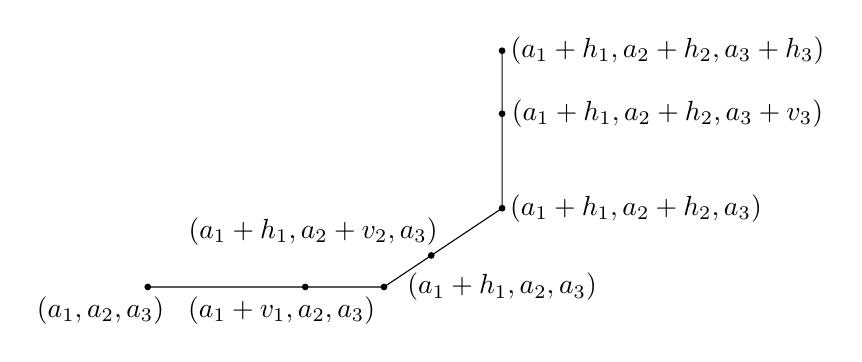
\begin{tikzpicture}
			\draw (0,0) -- (3,0) -- (4.5,1) -- (4.5,3);
			\draw[fill=black] (0,0) node[xshift=-6mm,yshift=-3mm]{$(a_1,a_2,a_3)$} circle (1pt);
			\draw[fill=black] (2,0) node[xshift=-3mm,yshift=-3mm]{$(a_1+v_1,a_2,a_3)$} circle (1pt);
			\draw[fill=black] (3,0) node[xshift=15mm,yshift=-0mm]{$(a_1+h_1,a_2,a_3)$} circle (1pt);
			\draw[fill=black] (3.6,0.4) node[xshift=-15mm,yshift=3mm]{$(a_1+h_1,a_2+v_2,a_3)$} circle (1pt);
			\draw[fill=black] (4.5,1) node[xshift=17mm]{$(a_1+h_1,a_2+h_2,a_3)$} circle (1pt);
			\draw[fill=black] (4.5,2.2) node[xshift=21mm]{$(a_1+h_1,a_2+h_2,a_3+v_3)$} circle (1pt);
			\draw[fill=black] (4.5,3) node[xshift=21mm]{$(a_1+h_1,a_2+h_2,a_3+h_3)$} circle (1pt);
		\end{tikzpicture}
	\end{center}

	Notice that $v_1,v_2,\dots,v_m$ are functions of $h$. Putting together we get
	\begin{align*}
		\dfrac{f(a+h)-f(a)-Th}{\|h\|} & = \frac1{\|h\|} \lt\langle h,\lt[ \begin{matrix}
				                                                                  \lt.\del{f}{x_1}\rt|_{v_1} -	\lt.\del{f}{x_1}\rt|_a \\
				                                                                  \vdots                                              \\
				                                                                  \lt.\del{f}{x_m}\rt|_{v_m}-	\lt.\del{f}{x_1}\rt|_a
			                                                                  \end{matrix} \rt]  \rt\rangle \\
		                              & =\frac1{\|h\|}\|h\|\|p-q\|=\|p-q\|
	\end{align*}
	Showing $\lim\limits_{h\to 0}\|p-q\|=0$ is enough to complete the proof $$ \lim\limits_{h\to 0}\|p-q\|=0\impliedby  p-q\to 0 \text{ as }h\to 0 \impliedby \lt.\del{f}{x_i}\rt|_{v_i} -	\lt.\del{f}{x_i}\rt|_a  \to 0\text{ as }h\to 0 $$ which is true because $\del{f}{x_i}$ is a continuous function. More formally choose $\|h\|<\delta$ s.t $$\lt\|\del{f}{x_i}(b)-	\del{f}{x_1}(a)\rt\| <\frac{\eps}{m}\ \forall \ b\in B_{\delta}(a)$$That ensures $\|p-q\|<\eps$ by triangle inequality.
	\qs{}{ \[ f(x,y)=\begin{cases}
				\frac{xy^2}{xx^2+y^4} & (x,y)\neq (0,0) \\
				0                     & \text{else}
			\end{cases}\]
		\begin{enumerate}
			\item Calculate all directional derivatives in particular $\del{f}{x},\del{f}{y}$
			\item Does $f'(a,b)$ exists at all $a,b\in \bbR$
			\item Is $f$ continuous everywhere
		\end{enumerate}
	}
\end{myproof}

\section{Higher Derivatives and Class \texorpdfstring{$C^k$}{Ck} functions}
Now we want to define class $C^k$  of functions for $k\geq 0$. [Like in 1-Variable case. Usefull for Taylor's theorem].

Now second derivative of $f:U\to\bbR^n$ at $a\in U\subset\bbR^m =$ derivative at $a$ of $f':U\to \mcL(\bbR^m,\bbR^n)\backsimeq \bbR^{mn}$. $\therefore$ $f''(a)$ or $D^2f(a):\bbR^m\to \mcL(\bbR^m,\bbR^n)$. Matrix of $f''(a)$ has $mn$ rows and $m$ columns and equals to $\deld{f'_{pq}}{x_j}$ where $p=1,\dots,n$, $q=1,\dots, m$ and $j=1,\dots, m$

\qs{}{Do $\deld{}{x_l}$ and $\deld{}{x_k}$ commute ?}
\solve{No but actually yes under some good conditions. We discussed here}

If $f''(a)$ exists for all $a\in U$, then  we get a  function $f''$ or $D^2f:U\to \mcL(\bbR^m,\mcL(\bbR^m,\bbR^n))$ which maps $a\mapsto f''(a)$. Dimension of the RHS is $m^2n$. Now we can ask about continuity and differentiability of $f''$

\dfn{$\bs{C^k}$ Functions}{Open $U\subset \bbR^m$, $f:U\to\bbR^n$. Then
	\begin{center}
		\begin{tabular}{rcl}
			$f$ is $C^0$ if        &                                           & $f$ is continuous       \\
			$f$ is $C^1$ if        & $f'(a)$ exists $\forall\ a\in U$ and      & $f'$ is continuous      \\
			$f$ is $C^2$ if        & $f''(a)$ exists $\forall\ a\in U$ and     & $f''$ is continuous     \\
			$\vdots$\hspace{0.5cm} & $\vdots$                                  & \hspace{1cm}$\vdots$    \\
			$f$ is $C^k$ if        & $f^{(k)}(a)$ exists $\forall\ a\in U$ and & $f^{(k)}$ is continuous
		\end{tabular}
	\end{center}

}

\nt{How to understand $\mcL(V,\mcL(U,W))$ where $U,V,W$ are vector spaces. Just set theoretically
	\begin{center}
		\large{\begin{tikzcd}[ampersand replacement=\&]
				\text{Maps}( \& [-1.1cm] A \& [-1.3cm] {,} \& [-1.3cm] \text{Maps}( \& [-1.1cm] B            \& [-0.8cm] {,} \& [-1.1cm] C                       \& [-1.4cm] )) \& [-1cm] \backsimeq      \& [-1.cm] \text{Maps}( \& [-1.1cm] A\times B \& [-0.8cm] {,} \& [-1.1cm] C  \& [-1.4cm] ) \\[-0.7cm]
				\&            \& \downarrow   \&                       \&                       \&              \&                                \&            \&                        \&                      \& \downarrow         \&              \&             \&            \\[-0.7cm]
				\&            \& f(a)         \& :                     \& B \arrow[rr]          \&              \& C \arrow[rrrr, Leftrightarrow] \&            \&                        \&                      \& \phi  \arrow[rr, maps to]   \&              \& {\phi(a,b)}  \&            \\[-0.7cm]
				\&            \&              \&                       \& b \arrow[rr, maps to] \&              \& {\phi(a,b)}                    \&            \&                        \&                      \&                    \&                \&
			\end{tikzcd}}
	\end{center}
	Under this dictionary, maps in $\mcL(V,\mcL(U,W))$ must correspond to some special kind of maps  $V\times U\to W$. }

Hence we can say $\mcL(\bbR^m,\mcL(\bbR^m,\bbR^n))$ is equivalent to the space of maps $\bbR^m\times \bbR^m\to \bbR^n$ which is space of bilinear maps from $\bbR^m\times \bbR^m$ to $\bbR^n$

Component functions of $f':U\to \mcL(\bbR^m,\bbR^n)$ are precisely $\del{f_i}{x_j}$ where $i=1,\dots, n$ and $j=1,\dots, m$. So matrix of $f''(a)$ w.r.t standard basis  of $\bbR^m$ and $\mcL(\bbR^m,\bbR^n)$ will consist of numbers $\lt(\deld{}{x_k}\lt(\deld{}{x_j}f_i\rt)\rt)(a)$. If $f''(a)$ exists   then these are generated to exist. If $f''(a)$ exists at each $a\in U$ then we have the function
\begin{center}
	\begin{tikzcd}
		{f'':} &[-1cm] U\arrow[r] & {\mcL(\bbR^m,\mcL(\bbR^m,\bbR^n))}\ &[-1.2cm] {\backsimeq\text{Space of bilinear maps }\bbR^m\times \bbR^m\to \bbR^n}\\[-0.7cm]
		&[-1cm] a \arrow[r, mapsto] & f''(a)
	\end{tikzcd}
\end{center}

$f''$ is $C^2(U) \overset{\text{definition}}{\iff} f''$ is continuous on $U\iff \deld{}{x_k}\deld{}{x_j}f_i$ are continuous  functions $U\to \bbR$
\begin{Theorem}{}{secdev}
	Let $U$ be open in $\bbR^2$ and $f:U\to \bbR$. $(a,b)\in \bbR$ and $U\supset Q(h,k)=[a,a+h]\times [b,b+k]$. Define \begin{align*}
		\Delta(h,k) & =f(a+h,b+k)-f(a,b+k)-f(a+h,b)+f(a,b)     \\
		            & =[f(a+h,b+k)-f(a+h,b)]-[f(a,b+k)-f(a,b)]
	\end{align*}Then $\exs$ $(s,t)\in $ interior of the rectangle $Q(h,k)$ such that $$\Delta(f,Q)=hk\lt( \del{}{y}\del{}{x}\rt)f(s,t)\coloneqq D_{21}f(s,t)$$
\end{Theorem}
\begin{proof}
	$U(x)=f(x,b+k)-f(x,b)$. Hence $$\Delta(f,Q)=U(a+h)-U(a)$$By $MVT$ we have  $s\in (a,a+h)$ such that \begin{align*}
		\Delta(f,Q) & =hU'(s)=h\lt[ \del{f}{x}(s,b+k)-\del{f}{x}(s,b) \rt]
	\end{align*}Apply $MVT$ again and we get $t\in (b,b+k)$ such that $$\del{f}{x}(s,b+k)-\del{f}{x}(s,b)=k\lt(\del{}{y}\del{}{x}\rt)f(s,t)$$And hence $$\Delta(f,Q)=hk\lt(\del{}{y}\del{}{x}\rt)f(s,t)$$
\end{proof}
\begin{Theorem}{}{}
	Suppose for $f$, $\del{f}{x}$, $\del{f}{y}$, $\del{}{y}\del{}{x}f$ exist everywhere and  $D_{21}f=\del{}{y}\del{}{x}f$ is  continuous  at $(a,b)$. Then $D_{12}f(a,b)=\lt.\del{}{x}\del{}{y}f\rt|_{a,b}$ exists and $$D_{21}f(a,b)=D_{12} f(a,b)$$
\end{Theorem}
\begin{proof}
	Let $\eps>0$ then  continuity of $D_{21}$ means that $\exs$ $\delta>0$  such that  $\forall\ h,k$ with $\max(|h|,|k|)<\delta$ $$\lt| D_{21}f(x,y)-D_{21}f(a,b)\rt|<\eps$$ $\forall\ x,y\in Q(h,k)$
	
	Take $h,k$ as above  and use the  \hyperref[th:secdev]{Theorem \ref{th:secdev}} to find $(s,t)$  such that $\Delta (f,Q)=hkD_{21}f(s,t)$. So $$\lt| \frac{\Delta(f,Q)}{hk}-D_{21}f(a,b) \rt|<\eps \text{ i.e. }
\Bigg| \frac{1}{h}\lt( \frac{f(a+h,b+k)-f(a+h,b)}{k}-\frac{f(a,b+k)-f(a,b)}{k} \rt) -D_{21}f(a,b)\Bigg| <\eps$$
Take limits as $k\to 0$ $$\lt|\frac1h \lt( \del{f}{y}f(a+h,b)-\del{f}{y}f(a,b) \rt)  -D_{21}f(a,b)\rt|<\eps$$As we take limit $h\to 0$ the quantity $\frac1h \lt( \del{f}{y}f(a+h,b)-\del{f}{y}f(a,b) \rt)$ actually exists  and is equal to $D_{21}f(a,b)$ i.e. $\del{}{x}\lt(\del{}{y}f(a,b)\rt)=D_{12}f(a,b)$ exists and is equal to $D_{21}f(a,b)$
\end{proof}
\begin{corolary}{}{}
	If $f$ is  $C^2(U)$ then $D_{21}f=D_{12}f$ at each point of $U$
\end{corolary}
\begin{Theorem}{}{}
	Let $U\subset \bbR^m$ and $f:U\to \bbR^n$ a $C^k$ map  i.e. $k-$th total derivative  $f^{(k)}$ exists and is continuous on $U$  then $$D_{i_1i_2\cdots i_k}f=D_{i_{\sigma(1)}i_{\sigma(2)}\cdots i_{\sigma(k)}}f$$e.g $D_{24714}f=D_{42417}(f)$
\end{Theorem}
\begin{proof}
	May take $m=1$ and work with component real valued functions for $k>2$ keep all but two variables fixed and use earlier result for requisite partial derivative of $f$. Any permutation can be realized as a sequence of transpositions
\end{proof}

\chapter{Multivariable Taylor Theorem}


In one variable $$f(a+h)=f(a)+f'(a)\frac{h}{1!}+f''(a)\frac{h^2}{2!}+\cdots+f^{(n-1)}(a)\frac{h^{n-1}}{(n-1)!}+f^{(n)}(c)\frac{h^n}{n!}$$ for a $c$ between $a,a+h$. 
\begin{theorem}{Multivariable Taylor Theorem}{taylor}	
	Let $U\subset \bbR^n$  open and $f:U\to \bbR^m$ a $C^m$ map ($m\geq 1$). Given $a\in U$, for any $h$ in some neighborhood  $W$ of origin, $O$ we have $W+a\subset U$ $$f(a+h)=f(a)+\EqM{c1}{f'(a)\frac{h}{1!}}+\EqM{c2}{f''(a)\frac{h^2}{2!}}+\cdots+f^{(m-1)}(a)\frac{h^{m-1}}{(m-1)!}+f^{(m)}(c)\frac{h^m}{m!}$$
	\begin{tikzpicture}[remember picture, 
		overlay
		]
		
		\draw[<-] ++(c1.south) -- ++(0,-2em)  node[xshift=-1.6cm,yshift=-.6cm] {$\lt[ \begin{matrix} D_1f(a) & D_2f(a)& \cdots & D_nf(a)  \end{matrix} \rt]\lt[ \begin{matrix}
				h_1\\ h_2\\ \vdots\\ h_n
			\end{matrix} \rt]$}; 
		\draw[<-] ++(c2.south) -- ++(0.7,-2em)  node[xshift=2cm,yshift=-0.35cm] {$\dfrac{\Sigma \text{ terms like } D_{ij}f(a)h_ih_j}{2!}$}; 
	\end{tikzpicture}
	\vspace{2cm}
	
	Hence $$f(a+h)=\sum_{k=0}^{m-1}\quad \sum_{s_1+s_2+\cdots+s_n=k} \frac{(D_1^{s_1}\cdots D_n^{s_n}f)(a)}{s_1!s_2!\cdots s_n!}h_1^{s_1}h_2^{s_2}\cdots h_n^{s_n}+\EqM{r}{r(h)}$$
	\begin{tikzpicture}[remember picture, 
		overlay
		]
		\draw[<-] ++(r.south) -- ++(0,-1em) node[yshift=-2mm] {remainder term};
	\end{tikzpicture}
	\vspace{1cm}
	
	where $r(h)$ is of the form $$\sum_{s_1+s_2+\cdots+s_n=m} \frac{(D_1^{s_1}\cdots D_n^{s_n}f)(a+\theta h)}{s_1!s_2!\cdots s_n!}h_1^{s_1}h_2^{s_2}\cdots h_n^{s_n}$$ where $\theta\in (0,1)$
\end{theorem}
\nt{$\frac{r(h)}{\|h\|^{m-1}}\to 0$ as $h\to 0$}
In one-variable $f:[a,b]\to \bbR$. Then $f^{(0)},f^{(1)},\dots, f^{(m-1)}$ exists in $[a,b]$ and $f^{(m)}
$ exists in $(a,b)$. Suppose $s,t\in [a,b]$. Then there exists $\theta$ exactly between $s$ and  $t$ such that $$f(t)=\underbrace{f(s)+f'(s)(t-s)+\cdots+\frac{f^{(m-1)}(s)}{(m-1)!}(t-s)^{m-1}}_{p(t)}+\frac{f^{(m)}(\theta)}{(m)!}(t-s)^{m-1}$$. Then  $$p(s)=f(s), p'(s)=f'(s),p''(s)=f''(s),\dots, p^{(m-1)}(s)=f^{(m-1)}(s)\text{ and }p^{(m)}(x)=0\text{ identically}$$So for $g(x)=f(x)-p(x)$ $$g(s)=g'(s)=\cdots =g^{(m-1)}(s)=0$$.\parinf

\textbf{\textit{Idea: }}Use $MVT$ on $g,g',\dots,g^{(m-1)}$ on $[s,t]$\parinn

\textbf{If} $g(t)=0$ then with $g(s)=0$ we get (by Rolle's theorem) $\theta_1$ between $s$ and $t$ such that $g'(\theta_1)=0$. Now $g'(\theta_1)=0$ and $g'(s)=0 \implies$ we get $\theta_2$ between $\theta_1$ and $s$ such that $g''(\theta_2)=0$.   Now $g''(\theta_2)=0$ and $g''(s)=0 \implies$ we get $\theta_3$ between $\theta_2$ and $s$ such that $g'''(\theta_3)=0$ and so on.. till we get $\theta_m$  with $g^{(m)}(\theta_m)=0$. Take $\theta=\theta_m$.

But is $g(t)=0$ ? $g(t)=f(t)-p(t)$ need not be zero.\parinf

\textbf{\textit{Idea:}} We can adjust $g$ by  constant  $M(x-s)^m$ without affecting $g(s)=g'(s)=\cdots =g^{(m-1)}(s)=0$ and we also want  to apply  the Rolle's theorem. Adjust constant $M$ to make $g(t)=0$\parinn

New $g(x)=f(x)-p(x)-M(x-s)^m$ such that $g(t)=f(t)-p(t)-M(t-s)^m=0$. Hence $$M=\frac{f(t)-p(t)}{(t-s)^m}$$We get $g^{(m)}(\theta)=f^{(m)}(\theta)-0-m!M=0$. S $$M=\frac{f^{(m)}(\theta)}{m!}$$Equate these two expressions  for $M$ and solve for $f(\theta)$ to get the result.

\qs{}{Carry out  proof of  multivariable taylor' theorem following the strategy  sketched  in the class, specially  using the chain  rule  to calculate $\frac{d^n}{dt^n}f(a+th)$}

\qs{}{In `some sense', the one-variable  Taylor's Theorem for $f(a+th)$ stays valid in multivariable  case.}

It is enough to proof for $m=1$. We have $a\in U\subseteq \bbR^n\xrightarrow{f}\bbR$, $f$ is $C^m$. Then there is a neighborhood $W$ of origin in $\bbR^n$  such that for any $h\in W$  we have $a+h\in U$ and  $$f(a+h)=f(a)+\EqM{c1}{f'(a)\frac{h}{1!}}+\EqM{c2}{f''(a)\frac{h^2}{2!}}+\cdots+f^{(m-1)}(a)\frac{h^{m-1}}{(m-1)!}+r(h)$$ where $r(h)=\frac{f^{(m)}(a+\theta h)}{m!}h^m$ for some $\theta\in (0,1)$ but need to make sense of this.

\begin{proof}
	Use one-variable taylor's theorem for the composite 
	
	\begin{center}
		\begin{tikzcd}
		{[0,1]} \arrow[r] & a+W\subset U\arrow[r, "f"] & \mathbb{R} \\
		t\arrow[r, maps to] & a+th\arrow[r, maps to] & f(a+th)=g(t)
	\end{tikzcd}
	\end{center}$g$ is $C^m$ because the map $t\mapsto a+th$ is $C^{\infty}$Hence $$f(a+h)=g(1)=\sum_{k=0}^{m-1}\frac{g^{(k)}(0)}{k!}+\frac{g^{(m)}(\theta)}{m!}$$for some $\theta\in (0,1)$. Thus we will be done by showing \begin{align*}
	g^{(k)}(t) &=\sum_{s_1+s_2+\cdots+s_n=k} \frac{k!}{s_1!s_2!\cdots s_n!}D_1^{s_1}\cdots D_n^{s_n}f(a+th)h_1^{s_1}h_2^{s_2}\cdots h_n^{s_n}\\
	&=\sum_{1\leq i_1,\dots,i_k\leq n}D_{i_1}\cdots D_{i_k}f(a+th)h_{i_1}h_{i_2}\cdots h_{i_n}
\end{align*}
Using chain rule for $k=1$ \begin{align*}
	g'(t) & =\frac{d}{dt}f(a+th)\\
	 &= f'(a+th)\frac{d}{dt}(a+th)\\
	 &=f'(a+th)h\\
	 &=\sum_{i=1}^nD_if(a+th)h_i
\end{align*}For $k=2$ \begin{multline*}
g''(t)+\frac{d}{dt}g'(t)=\frac{d}{dt}\sum_{i=1}^nD_if(a+th)h_i=\sum_{i=1}^n\frac{d}{dt}D_if(a+th)h_i\\
=\sum_{i=1}^n\sum_{j=1}^nD_jD_if(a+th)h_ih_j=\sum_{1\leq i,j\leq n}D_jD_if(a+th)h_i
\end{multline*}Continue like this
\end{proof}
\section*{Addendum to Taylor's Formula: Bounding the error term}
For $a\in U\subseteq \bbR^n$ and $f$ of class $C^m$ from $U$ to $\bbR$ we know that  for $h\in $ some ball $B$ around origin, we have $a+B\subset U$ and $$f(a+h)=\sum_{k=0}^{m-1}\quad \sum_{s_1+s_2+\cdots+s_n=k} \frac{(D_1^{s_1}\cdots D_n^{s_n}f)(a)}{s_1!s_2!\cdots s_n!}h_1^{s_1}h_2^{s_2}\cdots h_n^{s_n}+\EqM{r}{r(h)}$$where $r(h)$ is of the form $$\sum_{s_1+s_2+\cdots+s_n=m} \frac{(D_1^{s_1}\cdots D_n^{s_n}f)(a+\theta h)}{s_1!s_2!\cdots s_n!}h_1^{s_1}h_2^{s_2}\cdots h_n^{s_n}$$ where $\theta\in (0,1)$

Now because $a+\overline{B}$ is compact and $D_1^{s_1}\cdots D_n^{s_n}f$ is continuous  on $U$, we can find a constant $c$ such that for any $s_1,\dots,s_n$ with $\sum\limits_{i=)}^n =m$ $$\lt| \frac{D_1^{s_1}\cdots D_n^{s_n}f(a+x)}{s_1!s_2!\cdots s_n!}\rt|<c$$for each $h\in \overline{B}$ Also $|h_i|\leq \|h\|$. Therefore $$|r(h)|<\sum_{s_1+\cdots+s_n=m}c\|h\|^m=k\|h\|^m$$and therefore $\frac{r(h)}{\|h\|^{m-1}}\to 0$ as $h\to 0$


\chapter{Maximum and Minimum of Multivariable Functions}
For a $C^3$ function (in a neighborhood of $a$ in $\bbR$), by Taylor's Theorem $$f(a+h)=f(a)+f'(a)h+\frac12f''(a)h^2+\underbrace{\frac16f'''\lt(\begin{tabular}{c}\text{some point}\\ \text{between}\\ $a$ \text{ and } $a+h$\end{tabular}\rt)h^3}_{\substack{ \text{Remainder term }r(h) \\ \frac{r(h)}{h^2}\to 0 \text{ as }h\to 0}}$$Suppose $f'(a)=0$ ``$a$ is a critical point of $f$". Then
$$\frac{f(a+h)-f(a)}{h^2}=\frac12f''(a)+\frac{r(h)}{h^2}$$
If $f''(a)>0$ then $f$ has a local minimum at $a$ because choose $\delta >0$  such that $|h|<\delta$, $\lt|\frac{r(h)}{h^2}\rt|<\frac12f''(a)$. Then $RHS>0$ $\forall \ h$ such that $|h|<\delta$ and so for $h\in (-\delta,\delta)$, $f(a+h)>f(a)$ i.e. $f(a)$ is minimum value of $f$ in the neighborhood $(a-\delta,a+\delta)$. Similarly $f''(a)<0$ then $f$ has  a local maximum  at $a$. 


We want to find an analogy  of this for multivariable case

$f:(\text{open }U\text{ in }\bbR^n )\to \bbR$ a $C^3$ function. Then  for $h\in $ some  open neighborhood $W$ of origin, $a+h\in U$ \begin{align*}
	f(a+h) & =f(a)+f'(a)h+\frac12f''(a)(h,h)+\underbrace{\frac16f'''\lt(\begin{tabular}{c}
		  \text{some point}    \\
		    \text{between}     \\
		$a$ \text{ and } $a+h$
	\end{tabular}\rt)(h,h,h)}_{\substack{ \text{Remainder term }r(h) \\ \frac{r(h)}{h^2}\to 0 \text{ as }h\to 0}} \\
	& = f(a)+\lt[ \begin{matrix}
		D_1 & \cdots & D_n
	\end{matrix} \rt]\lt[ \begin{matrix}
	h_1\\ \vdots \\ h_n
\end{matrix} \rt]+\frac12 \sum_{i,j}D_iD_jf(a)h_ih_j+r(h)\\
&=  f(a)+\lt[ \begin{matrix}
	D_1 & \dots & D_n
\end{matrix} \rt]\lt[ \begin{matrix}
	h_1\\ \vdots \\ h_n
\end{matrix} \rt] +\frac12 \lt[ \begin{matrix}
h_1& \cdots & h_n
\end{matrix}\rt][D_iD_jf(a)] \lt[ \begin{matrix}
h_1\\ \vdots\\ h_n
\end{matrix} \rt]+r(h)\\
&=f(a)+\nabla f(a)\cdot h+\frac12 h^T \underbrace{[D_iD_jf(a)]}_{\substack{\text{Hessian Matrix}\\ \text{of }f\text{ at }a}}h+r(h)
\end{align*}
\dfnc{Hessian Matrix of $f$}{
	Let $f:(\text{open }U\text{ in }\bbR^n )\to \bbR$ such that $\begin{cases}
		f\text{ is }C^1\iff \deld{f}{x_i}\text{ are not continuous on }U\\
		f'' \text{ exists at }a
	\end{cases}$ So components of $f''$ are $D_iD_jf(a)$. Hessian of $f$ at $a$ = Square matrix $[D_iD_jf(a)]$
}
When $f$ is $C^2$, Hessian matrix is Symmetric Matrix

\dfnc{Critical Point}{
Let $f$ be a $C^1$ function, Open $U$ in $\bbR^n\xrightarrow{f}\bbR$. $a\in U$ is called critical point if $f'(a)=0\iff \nabla f(a)=0$
}
If $f$ has local maximum  at $a$, then along any line through $a$ the same must be hold, so all directional derivative =0 at $a$.
\dfnc{Non-degenerate Point}{If $f$ is $C^2$  then a critical point $a$  is called non-degenerate if the Hessian, $Hf(a)$ is non-singular i.e. $\det(Hf(a))\neq 0$
}

\begin{Claim}{}{}
	Symmetric Matrix  $A$ is positive (semi)definite $\iff $ $\forall$ nonzero vector $x\in \bbR^n$, $x^TAx>0$ (resp. $\geq 0$)
\end{Claim}
\begin{proof}
	\subsubsection*{If Part:}
	$x=\sum\limits_{i}c_iv_i$. Where $v_i$ is the eigen-basis. Then \begin{align*}
		x^TAx & = \lt(\sum\limits_{i}c_iv_i\rt)^TA\lt(\sum\limits_{j}c_jv_j\rt) = \lt(\sum\limits_{i}c_iv_i\rt)^T\lt( \sum_j\lm_jc_jv_j \rt) = \sum_i\lm_ic_i^2>0 \qquad [v_i^Tv_j=\delta_{ij}]
	\end{align*}
\subsubsection*{Only If Part:}
Use $x^TAx>0$  for $x=v_i$ eigenvector $<0,$ $v_i^TAv_i=v_i\lm_iv_i=\lm_i$
\end{proof}
\nt{Determinant of positive definite matrix $>0$ and Determinant of negative definite matrix has sign $(-1)^n$}



\begin{theorem}{}{maxminif}
Let $f:(\text{open }U\text{ in }\bbR^n )\to \bbR$. Suppose $f $ has a local maximum or minimum  at $a$  then \begin{enumerate}[label=\bfseries\tiny\protect\circled{\small\arabic*}]
	\item If $f'(a)$ exists then $f'(a)=0$ i.e. $a$ is a critical point. 
	\item Suppose in addition to that $f''(a)$  exists then if $f$ has local maximum at $a$, then $f''(a)\leq 0$ and if $f$ has local minimum at $a$, then $f''(a)\geq 0$
\end{enumerate}
\end{theorem}
\begin{proof}
	\begin{enumerate}[label=\bfseries\tiny\protect\circled{\small\arabic*}]
		\item For $n=1$  let we have local minimum at $a$. Then for small $|h|$
		
		\begin{center}
			 $\begin{rcases}
			 	\frac{f(a+h)-f(a)}{h}\geq 0 & \text{ for }h>0 \\
			 	\frac{f(a+h)-f(a)}{h}\leq 0 & \text{ for }h<0
			 \end{rcases}$Thus imply respectively that $f'(a)$  must be $\geq 0$ and $\leq 0$
		\end{center}
	For $n>1$  use $n=1$ in every direction i.e. for function $\lt. f\rt|_{a+tv}$ for $t\in $ open interval  to conclude $D_vf(a)=0$ $\forall$ directions. So $f'(a)=0$\Qed
	\item For $n=1$ $$f''(a)=\lim\limits_{h\to 0}\frac{f'(a+h)-f'(a)}{h}=\lim\limits_{h\to 0}\frac{f'(a+h)}{h}$$ 
	\parinf 
	
	\textbf{\textit{Observation: }}If $f$ has local maximum at $a$ then for $0<|h|<\delta$, $f(a+h)\geq f(a)$. So by $MVT$  there is $k$ between $0$ and $h$  such that $$\frac{f(a+h)-f(a)}{h}=f'(a+k)$$\parinn
	
	Using the observation $f''(a)=\lim\limits_{h\to 0}\frac{f'(a+k)}{h}\geq 0$
	
	For $n>1$ applying this  to each $\lt. f\rt|_{a+tv}$ $\forall$ direction vectors $v$  we get all $D^2_vf(a)\geq 0$. In terms of Hessian  let $v=\sum c_ie_i\implies D_vf=\sum c_iD_if\implies D^2f(a)=\sum_{i,j}c_jc_iD_jD_if(a) $ in  a neighborhood of $a$. $$D^2_vf(a)=\lt[ \begin{matrix}
		c_1 & \cdots & c_n
	\end{matrix} \rt]Hf(a)\lt[ \begin{matrix}
	c_1\\ \vdots\\ c_n
\end{matrix} \rt]$$
	\end{enumerate}
\end{proof}

\begin{theorem}{}{}
If $f:(\text{open }U\text{ in }\bbR^n )\to \bbR$ is a $C^3$  function  and $a$ is a non-generate critical point  of $f$  then 



\begin{center}
	\begin{tabular}{rcl}
		$f$ has a local minimum at $a$ & $\iff$ & $H$ is positive definite            \\
		                               & $\iff$ & All eigenvalues of $H$ are positive \\
		$f$ has a local maximum at $a$ & $\iff$ & $H$ is negative definite            \\
		                               & $\iff$ & All eigenvalues of $H$ are negative \\
		$f$ has saddle-point otherwise &        & $H$ is indefinite
	\end{tabular}
\end{center}
\end{theorem}
\begin{proof}
	\subsubsection*{If Part:}
	We already proved the if direction in \hyperref[th:maxminif]{Theorem \ref{th:maxminif}}
	
	\subsubsection*{Only If Part:}
	By Taylor's theorem $$f(a+x)-f(a)=\cancelto{0}{f’(a)}x+\frac12x^THx+r(x)$$with as $\|x\|\to 0$, $\frac{r(x)}{\|x\|^2}\to 0$. Let's assume that $H$ is positive definite. So far $x\neq 0$ and $x^THx>0$. 
	The function $x\to x^THx$ is continuous, so on the compact set $\{u\mid \|u\|=1\}$ it is bounded and achieves its infimum $\mu$. So $\mu>0$ So $$\frac{x^THx}{\|x\|^2}\geq \mu\ \forall \ x\neq 0\implies \lt(\frac{x}{\|x\|}\rt)^TH\lt( \frac{x}{\|x\|} \rt)$$ Since $\frac{r(x)}{\|x\|^2}\to 0$ as $\|x\|\to 0$, we can find $\delta>0$ such that $\frac{|r(x)|}{\|x\|^2}<\frac{\mu}{2}$ when $\|x\|<\delta$. Thus for $\|x\|<\delta$ we have $f(a+x)-f(a)\geq 0$ i.e. $f$ has a local minimum at $a$
\end{proof}

\dfnc{Saddle Point}{At  a nondegenrate critical point $a$, $H$ has both \begin{center}
		\begin{tabular}{c}
		$a$ positive eigenvalue, say $\lm_1$ with eigen vector $u_1$\\
		$a$ negative eigenvalue, say $\lm_2$ with eigen vector $u_2$
\end{tabular}
	\end{center}This means $D^2_{u_1}f(a)>0$, so in the $u_1$ direction $f$ has local minimum and $D^2_{u_2}f(a)<0$, so in the $u_2$ direction $f$ has local maximum

\begin{center}
	\includegraphics[width=6cm]{images/saddle.pdf}
\end{center}
}
\exc{}{Many times functions are $C^{\infty}$ whenever defined so all of the above applies.\begin{itemize}
		\item $f(x,y)=c,$ constant. All derivatives are zero, $H$ is zero.
		\item $f(x,y)=ax+by+c$ linear, $(a,b)\neq (0,0).$ No critical points.
		\item $f(x,y)=$ quadratic.
		
		General case $(x_1,x_2,\dots,x_n)=x\in\bbR^n$ \begin{align*}
			\Phi(x) &  =\sum_{i=1}^na_{ii}x_i^2+\sum_{1\leq i<j\leq n}2a_{ij}x_ix_j+\sum_{i=1}^np_ix_i+r\\
			& = x^TAx+px+r\\
			& =\lt[ \begin{matrix}
				x_1 & \cdots & x_n
			\end{matrix} \rt]\lt[ \begin{matrix}
			a_{11} & \cdots & a_{1n}\\ \vdots & \ddots & \vdots\\ a_{n1} & \cdots & a_{nn}
		\end{matrix} \rt]\lt[ \begin{matrix}
		x_1 \\ \vdots \\ x_n
	\end{matrix} \rt]+\lt[ \begin{matrix}
	p_1 &\cdots & p_n
\end{matrix} \rt]\lt[ \begin{matrix}
x_1 \\ \vdots \\ x_n
\end{matrix} \rt]+r \quad [\text{where }a_{ij}=a_{ji}]
		\end{align*}
	Hence $D_i\Phi(x)=\sum_{j=1}^n a_{ij}x_j+p_i$, $D\Phi(x)=2Ax+p$.	Critical points: $x$ such that $2Ax_p=0$
	
	If $2A=H$ is nonsingular then there is an unique critical point, namely $x=-H^{-1}p$. Then this point is local minimum is $H$ is positive definite, local maximum id $H$ is negative definite and saddle point otherwise
	\end{itemize}

}

\chapter{Examples of Functions and Analyze Critical Points}
Graph of $\Phi(x)=\Phi(x_1,\dots, x_n)$ is in $\bbR^{n+1}$. We can visualize it in $\bbR^n$ by drawing level sets, namely plot $\Phi(x_1,\dots,x_n)=c$ for various values of constant $c$ in $\bbR$
\section*{Examples}
\begin{enumerate}[label=\bfseries\tiny\protect\circled{\small\arabic*}]
	\item $f(x,y)=x^2$
	
	\begin{center}
		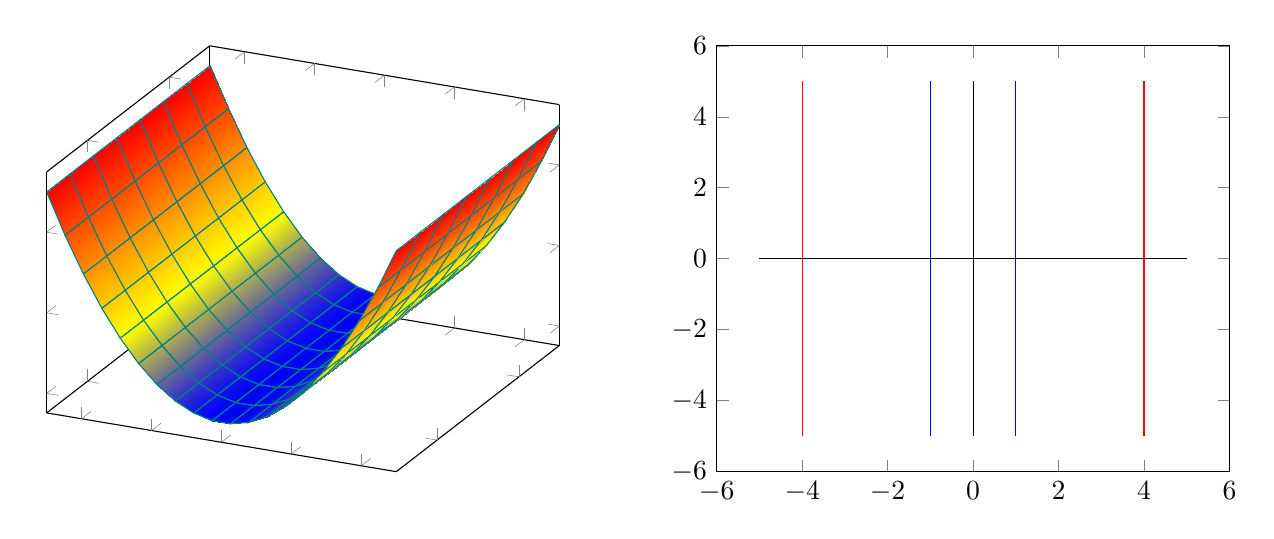
\begin{tikzpicture}
			
			\begin{axis}[scale=0.95,name=Ax1,ymax=0.99,xticklabels={\empty},yticklabels={\empty},zticklabels={\empty}]
				
				\addplot3 [
				domain=-5:5,
				domain y = -3:1,
				samples = 20,
				samples y = 8,
				surf,
				shader = faceted interp,
				faceted color = teal] {x^2};
				
			\end{axis}
		\begin{axis}[scale=0.95,name=Ax2,at={($(Ax1.north east)+(2cm,0)$)},anchor=north west] 
			\addplot[red] (4,x); 
			\addplot[red] (-4,x); 
			\addplot[blue] (1,x); 
			\addplot[blue] (-1,x); 
			\addplot[black] (0,x); 
			\addplot[black]{0};
		\end{axis}
			
		\end{tikzpicture}
	\end{center}

\item $f(x,y)=x^2+y^2$. Level Sets = Circles centered at $(0,0)$
\begin{center}
	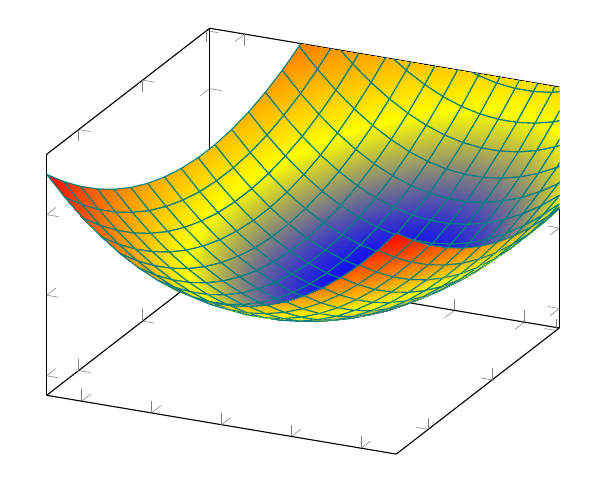
\begin{tikzpicture}
		
		\begin{axis}[scale=0.95 ,name=Ax1,ymax=0.99,xticklabels={\empty},yticklabels={\empty},zticklabels={\empty}]
			
			\addplot3 [
			domain=-50:50,
			domain y = -50:50,
			samples = 20,
			samples y = 20,
			surf,
			shader = faceted interp,
			faceted color = teal] {x^2+y^2};
			
		\end{axis}

		
	\end{tikzpicture}
\end{center}
\item $f(x,y)=x^2-y^2$. Level Sets $c=0\implies x=\pm y$, $c=1\implies x^2-y^2=1$, $c=-1\implies x^2-y^2=-1$
\vspace{1cm}

\begin{center}
	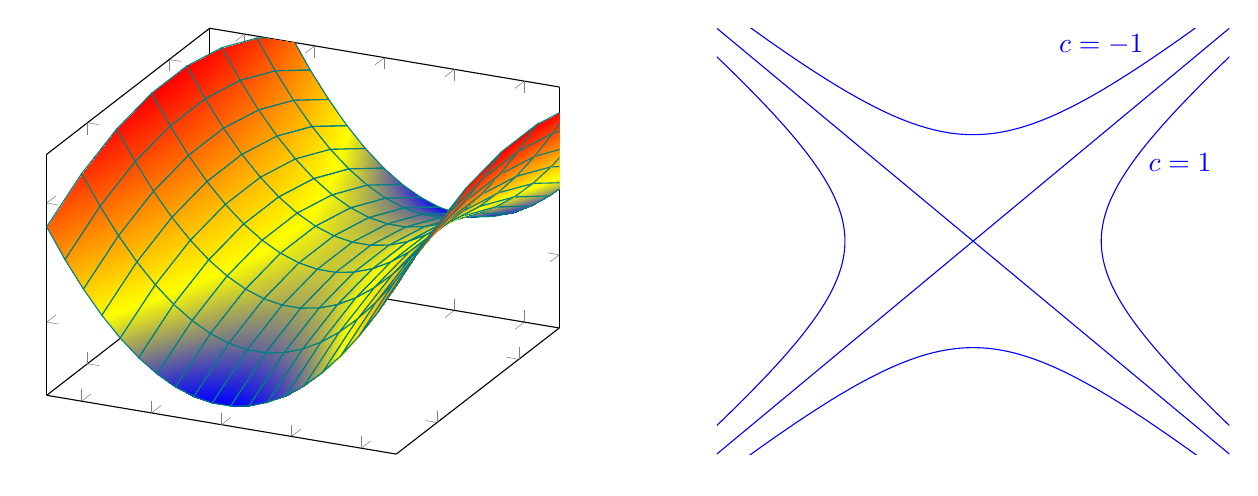
\begin{tikzpicture}
	\begin{axis}[scale=0.95,name=Ax1,ymax=0.99,xticklabels={\empty},yticklabels={\empty},zticklabels={\empty}]
		
		\addplot3 [
		domain=-5:5,
		domain y = -3:3,
		samples = 20,
		samples y = 8,
		surf,
		shader = faceted interp,
		faceted color = teal] {x^2-y^2};
		
	\end{axis}
	\begin{axis}[scale=0.95,name=Ax2,at={($(Ax1.north east)+(2cm,0)$)},anchor=north west,hide axis,xmin=-2,xmax=2,ymin=-2,ymax=2,restrict x to domain=-10:10]
		\addplot[blue, variable=t,domain=0:360,samples=200] ({sec(t)}, {tan(t)}) node[xshift=1cm, yshift=1cm]{$c=1$} node[xshift=0cm, yshift=2.5cm]{$c=-1$};
		\addplot[blue,variable=t,domain=0:360,samples=200] ({tan(t)}, {sec(t)});
		\addplot[blue]{x};
		\addplot[blue]{-x};
	\end{axis}
\end{tikzpicture}
\end{center}
\item $f(x,y)=xy$

$u=\frac{x+y}{\sqrt{2}},v=\frac{x-y}{\sqrt{2}}$. Then $x=\frac{u+v}{\sqrt{2}},y=\frac{u-v}{\sqrt{2}}$ and $f(x,y)=\frac{u^2-v^2}{2}$. Here $A=\frac12\lt[ \begin{matrix}
	0 &1\\ 1 &0
\end{matrix} \rt]$. Hence eigenvectors are $\lt[ \begin{matrix}
1\\ 1
\end{matrix} \rt]$ and $\lt[ \begin{matrix}
1\\ -1
\end{matrix} \rt]$

\begin{center}
	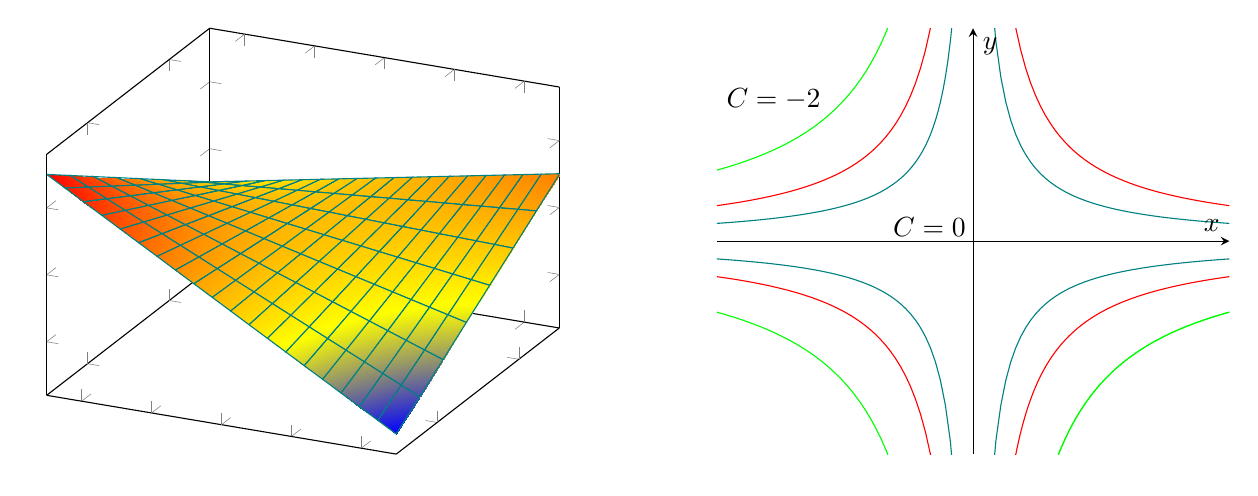
\begin{tikzpicture}
		\begin{axis}[scale=0.95,name=Ax1,ymax=0.99,xticklabels={\empty},yticklabels={\empty},zticklabels={\empty}]
			
			\addplot3 [
			domain=-5:5,
			domain y = -3:1,
			samples = 20,
			samples y = 8,
			surf,
			shader = faceted interp,
			faceted color = teal] {x*y};
			
		\end{axis}
		\begin{axis}[scale=0.95,name=Ax2,at={($(Ax1.north east)+(2cm,0)$)},anchor=north west,
			axis x line=center,
			axis y line=center,
			xlabel = $x$,
			ylabel = {$y$},
			ymax=3,
			ymin=-3,
			ticks=none,
			]
			\node[right] at (-2,2) {$C=-2$};
			\node[right] at (-0.7,0.2) {$C=0$};
			
			%Below the red is defined
			\addplot [
			domain=-2:-0.1, 
			samples=50, 
			color=red,
			]
			{1/x};
			\addplot [
			domain=0.1:2, 
			samples=50, 
			color=red,
			]
			{(1/x)};  
			\addplot [
			domain=-2:-0.1, 
			samples=50, 
			color=red,
			]
			{ -1/x};
			\addplot [
			domain=0.1:2, 
			samples=100, 
			color=red,
			]
			{(-1/x)};
			
			% Now the teal
			\addplot [
			domain=-2.:-0.1, 
			samples=50, 
			color=teal,
			]
			{(0.5/x)};
			\addplot [
			domain=0.1:2, 
			samples=50, 
			color=teal,
			]
			{(0.5/x)};
			\addplot [
			domain=-2:-0.1, 
			samples=100, 
			color=teal,
			]
			{ -0.5/x};   
			\addplot [
			domain=0.1:2, 
			samples=50, 
			color=teal,
			]
			{(-0.5/x)};
			
			%Here green  is defined
			\addplot [
			domain=-2:-0.1, 
			samples=50, 
			color=green,
			]
			{-2/x};
			\addplot [
			domain=-2:-0.1, 
			samples=50, 
			color=green,
			]
			{2/x};
			\addplot [
			domain=0.1:2, 
			samples=50, 
			color=green,
			]
			{-2/x};
			\addplot [
			domain=0.1:2, 
			samples=50, 
			color=green,
			]
			{-2/x};
			
		\end{axis}
	\end{tikzpicture}
\end{center}
\end{enumerate}

We should understand graphs of `Quadratic Hypersurfaces' $\Phi(x)=0$, where $\Phi(x)$ is  a quadratic polynomial in $n$ variables. 

`Standard Form' is $\lm_1x_2^2+\lm_2x_2^2+\cdots+\lm_nx_n^2+$ Constant. We will see that by a shift of origin and orthogonal change of coordinates, we can express any general quadratic $\Phi$ to the Standard Form
\begin{enumerate}[label=\bfseries\tiny\protect\circled{\small\arabic*}]
	\item Getting Rid of Linear Part
	
	\begin{align*}
		& \lm_1x_1^2+\lm_2x_2^2+\cdots+\lm_nx_n^2+p_1x_1+\cdots+p_nx_n+\text{ constant}\\
		= & \lm_1(x_1-a_1)^2+\cdots+\lm_n(x_n-a_n)^2+\text{ another constant} \quad [-2\lm_ia_i=p_i\implies a_i=-\frac{p_i}{2\lm_i},\text{ assuming }\lm_i\neq 0]
	\end{align*}
\item In general we express $x$ in terms of new basis consisting of orthonormal eigenvectors of $A$. 

Nationalizing a matrix $A$, $\Gamma^{-1}A\Gamma=D $-diagonal matrix where columns of $\Gamma=$ eigen basis corresponding to matrix $A$. Here $\Gamma$ is orthogonal matrix $\Gamma\Gamma^T=\Gamma^T\Gamma=I$ and we have $\Gamma^TA\Gamma=D\implies A=\Gamma D\Gamma^T$. Now $$\Phi(x)=x^TAx+pX+r$$Let $x^*=$ coordinate vector of $x$ in terms of  new basis consisting of columns of $\Gamma$\begin{align*}
	x^* & = \Gamma^{-1}x=\Gamma^T x \text{ we use this to formulate }\Phi\\
	& = (x^T\Gamma)D(\Gamma^Tx)+p\Gamma(\Gamma^Tx)+r=\Phi(x)\\
	& = \underset{  \substack{  \downarrow \\ \text{standard} \\ \text{form}  }  }{{x^*}^TDx^*}+\underset{\substack{\downarrow \\ \text{linear} \\ \text{form}  }  }{p\Gamma x^*}+r=\Psi(x^*)
\end{align*} Use step 1 to eliminate the linear term
\end{enumerate}

Now we will look into some more examples.
\begin{enumerate}[label=\bfseries\tiny\protect\circled{\small\arabic*}]
	\item $f(x,y)=x^2-xy+y^2$
	
	$$A=\lt[ \begin{matrix}
		1 & -\frac12\\ -\frac12 & 1
	\end{matrix} \rt]\text{ and }H=\lt[ \begin{matrix}
	1 & -1\\ -1 & 2
\end{matrix} \rt]$$ $H$ is  positive definite because diagonal entries are positive and determinant $ =3>0$. So the unique critical point $(0,0)$ is a local minima
\nt{
$2\times 2$ symmetric matrix $\lt[ \begin{matrix}
	a & c\\ c& b
\end{matrix} \rt]$ is positive definite $\iff \begin{cases}
a,b>0\\ ab-c^2>0
\end{cases}$
}

\item $\Phi(x)=2x^2+3y^2-4xy-12x-14y+21=\mat{x\\y}^TA\mat{x\\ y}+p\mat{x\\ y}+r$

$$A=\mat{2& -2\\ -2 & 3}\text{ and }H=\mat{4 & -4\\ -4 & 6}\text{ and }p=\mat{ -12 & 14}$$ $H$ is positive definite as diagonal entries are positive and determinant $=8>0$. The critical point is the solution of the equation $$H\mat{x\\ y} = - \mat{ -12 \\ 13} \iff \mat{4 & -4\\ -4 & 6}\mat{x\\ y}=-\mat{-12\\ 14}$$Hence $x=2$, $y=-1$. Therefore minimum value $\Phi(2,-1)=2$
\nt{
Another way: Complete the squares \begin{align*}
	\Phi(x) & = 2(x-2)^2+4(y+1)^2-4(x-2)(y+1)+2\\
	& = 2u^2+3v^2-4uv+2
\end{align*}}
\item $f(x,y)=x^3+y^3-3x-3y$

$$f'(x,y)=\mat{3x^2-3 & 3y^2-3}, \qquad \nabla f=\mat{3x^2-3\\ 3y^2-3}$$Critical points are $(x,y)$ such that $f'(x,y)=0$ i.e. $\begin{cases}
	3x^2-3=0\\ 3y^2-3=0
\end{cases}$. There are 4 critical points $=(\pm 1, \pm 1)$ $$\text{Hessian }H=\mat{6x & 0\\ 0 & 6x}$$ \begin{center}
\begin{tabular}{l}
	$(1,1,)\to$ local min, 	$(-1,-1)\to$ local max, $(\pm 1,\mp 1)\to$ saddle points
\end{tabular}
\end{center}
 \end{enumerate}
\nt{For $x^3-y^2+3x-3y$ there are no critical points}

\chapter{Constrained Optimizations and Lagrange Multipliers}
\parinf

\textbf{\textit{Example: }}Optimize $f(x,y)y^2-x^2$ subject to the constraint $h(x,y)=x^2+y^2=1$
\parinn

\begin{center}
	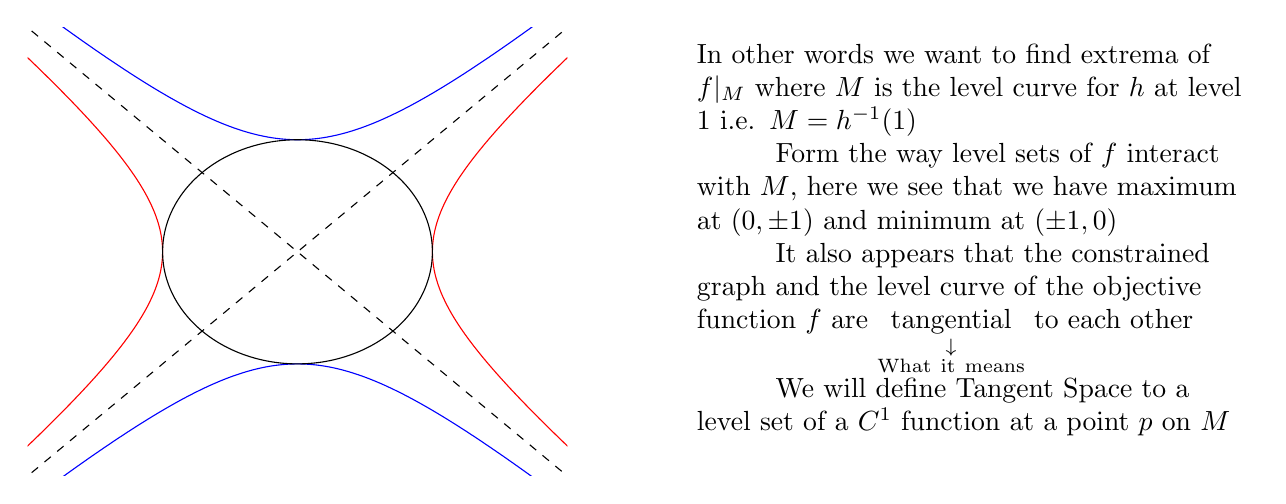
\begin{tikzpicture}
		
		\begin{axis}[xmin=-2,xmax=2, ymin=-2, ymax=2,
			restrict x to domain=-10:10, hide axis]% remove crossing lines at t=90 and t=270
			\addplot[red, variable=t,domain=0:360,samples=200] ({sec(t)}, {tan(t)});
			\addplot[blue,variable=t,domain=0:360,samples=200] ({tan(t)}, {sec(t)});
			\addplot[dashed]{x};
			\addplot[dashed]{-x};
			\addplot[variable=t,domain=0:360,samples=200]  ({cos(t)}, {sin(t)}) ;
		\end{axis}
	\node[text width=7cm, xshift=12cm,yshift=3cm]{\parindent=1cm In other words we want to find extrema of $f|_M$ where $M$ is the level curve for $h$ at level 1 i.e. $M=h^{-1}(1)$
	
Form the way level sets of $f$ interact with $M$, here we see that we have maximum at $(0,\pm 1)$ and minimum at $(\pm 1,0)$

It also appears that the constrained graph and the level curve of the objective function $f$ are $\underset{ \substack{ \downarrow \\ \text{What it means} } }{\text{tangential}}$ to each other

We will define Tangent Space to a level set of a $C^1$ function at a point $p$ on $M$
};
	\end{tikzpicture}
\end{center}
\section{Tangent Space}
\dfn{Tangent Space}{Tangent Space to a hypersurface $M=f^{-1}(c)$ in $\bbR^n$ where $f:(\text{Open }U\subset \bbR^n)\to \bbR$ is a $C^1$ function and $c\in \bbR$ at a point $p\in M$ is a subspace of $\bbR^n$ defined to be $$T_pM=\ker (f'(p))=\{v\in\bbR^n\mid f'(p)(v)=0\}=\{v\in \bbR^n\mid \nabla f(p)\cdot v=0\}$$}
Geometric tangent space considering to our mental image = $T_pM+p=$ Shift $T_pM$ by vector $p$. Likewise define Normal Space to be the set of vectors orthogonal to $T_pM$ i.e. $T_pM^{\perp}$

\begin{center}
	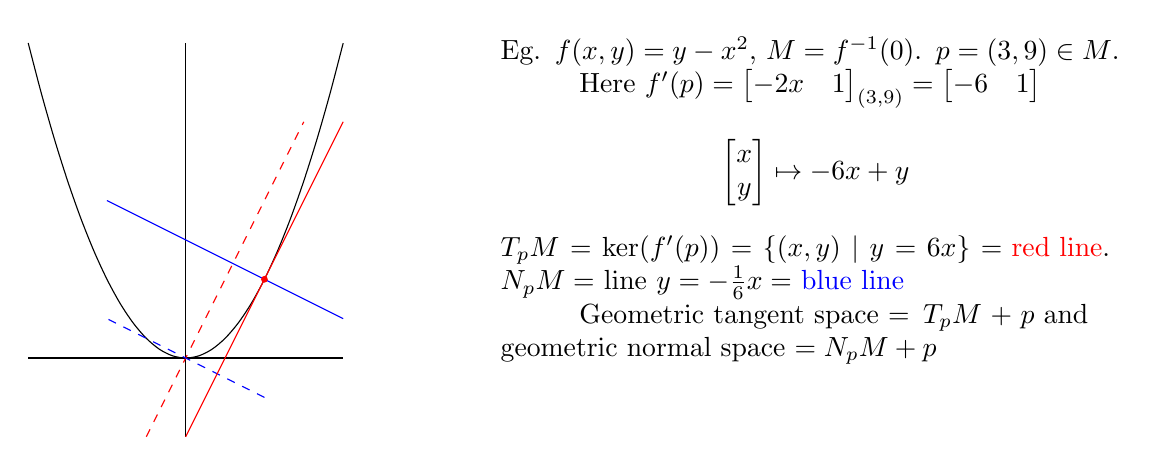
\begin{tikzpicture}
		\draw[domain=-2:2, smooth, variable=\x] plot ({\x}, {\x*\x});
		\draw (-2,0) -- (2,0);
		\draw (0,4) -- (0,-1);
		\draw[red,dashed] (-0.5,-1) -- (1.5,3);
		\draw[blue,dashed] (1,-0.5) -- (-1,0.5);
		\draw[red] (0,-1) -- (2,3);
		\draw[blue] (2,0.5) -- (-1,2);
		\filldraw[red] (1,1) circle (1pt);
		\node[text width=8cm, xshift=8cm,yshift=2cm]{\parindent=1cm 
		Eg. $f(x,y)=y-x^2$, $M=f^{-1}(0)$. $p=(3,9)\in M$. 
		
		Here $f'(p)=\mat{-2x & 1}_{(3,9)}=\mat{-6& 1}$ $$\mat{x \\ y} \mapsto -6x+y$$ $T_pM=\ker(f'(p))=\{ (x,y)\mid y=6x\}=$ \textcolor{red}{red line}. $N_pM= $ line $y=-\frac16 x =$ \textcolor{blue}{blue line}
		
		Geometric tangent space $=T_pM+p$ and geometric normal space $=N_pM+p$
	};
	\end{tikzpicture}
\end{center}
\section{Lagrange Multiplier}
Let $U$ be open in $\bbR^n$. $f:U\to \bbR$ objective function and $h:U\to \bbR$ constraint function. Want to find extrema of $f$ restricted to the level set $M=\{x\in U\mid h(x)=c\}=h^{-1}(c)$ for $c\in\bbR$

$f|_M$ has local maxima at $p\in M$ means for some $W\subset  U$,  $f(p)\geq f(x)\ \forall \ x\in W\cap M$
\dfn{$C^1$ Path and Velocity Vector}{A $C^1$ path centered at $p\in U$ in $U\subset \bbR^n$ is a $C^1$ map $\gm:(-\veps,\veps)\to U$ where $0\mapsto p$. We call $\gm'(0)=$ velocity of $\gm$ at 0}
\thm[lagmult]{Lagrange Multiplier}{
Let $U$ be open in $\bbR^n$. $f:U\to \bbR$, $h:U\to \bbR$. Let $f,h$ are $C^1$ functions. Let $M=h^{-1}(c)$. If $h'(p)\neq 0$ and $f|_M$ has  a local extrema  at $p\in M$  then  $\exs!\lm\in \bbR$ such that $$\nabla f(p)=\lm \nabla h(p)$$
}
\begin{proof}
Consider paths on level set $M=h^{-1}(c)$ i.e. \begin{center}
	\begin{tikzcd}[column sep={3em},/tikz/column 1/.style={column sep=0},/tikz/column 3/.style={column sep=0em}]
	\gm: &  (-\veps,\veps) \arrow[r] \arrow[rdd]&  M &=h^{-1}(c)\\[-8mm]
	 &  & \cap & \\[-8mm]
	 && U \arrow[r, "h"] & \bbR
\end{tikzcd}
\end{center}
Then $h=\gm(t)=c$ $\forall\ t\in (-\veps,\veps)$. Hence by Chain Rule $$h'(p)\gm'(0)=\nabla h(p)\cdot \gm'(0)=0$$ i.e. $\{\text{velocity vectors of all paths }\gm\text{ on }M\text{ centered at }p\}\subset T_pM$\parinf

\textbf{\textit{Key Fact: }}When $h'(p)\neq 0$ we have equality! Proof of this fact uses \hyperref[th:implicit]{Implicit Function Theorem}\parinn

Now let's recall the objective function $f$ and recall that $p$ is assured to be a local max/min. If $\gm$ is a $C^1$ curve on $M$ then in particular $f|_{\text{image}(\gm)}$ also has a max/min at $p$. Therefore $$0=(f\circ \gm)'(o)=\nabla f(p)\cdot \gm'(0)$$i.e. $\nabla f$ is orthogonal to velocity vectors to all curves centered at $p$. 

By claim $\nabla f(p)\perp T_pM$, we already  say $\nabla h(p)\perp T_pM$. We know $\nabla h(p)\neq 0$ by assumption. Hence $\exs! \lm$ such that $\nabla f(p)=\lm \nabla h(p)$
\end{proof}

\section{Some Examples for Applications}
\begin{enumerate}[label=(\roman*)]
	\item $f(x,y)=y^2-h^2$ and $h(x,y)=x^2+y^2$, $c=1$. Therefore $M=h^{-1}(1)=$ Unit Circle
	
	Suppose $p=\mat{a\\ b}$ is an extremum of $f|_M$ $$\nabla f(p)=\mat{-2x\\ 2y}_{(a,b)} = \mat{-2a\\ 2b}\qquad \nabla h(p)=\mat{2x\\ 2y}_{(a,b)} = \mat{2a\\ 2b}$$ We know that $\exs ! \lm \in \bbR$ such that $$\mat{-2a\\ 2b}=\lm \mat{2a\\ 2b}$$ This is not possible unless one of $a,b$ os 0. Therefore \begin{center}
		\begin{tabular}{lcl}
			$a=0$ & $\implies $ &$b=\pm 1$ and $\lm=1$\\
			$b=0$ & $\implies$ & $a=\pm 1$ and $\lm=-1$
		\end{tabular}
	\end{center}
\item $f(x,y)=y$ is subject to constraint $h(x,y)=y-g(x)=0$ where $g:\bbR\to \bbR$ is some $C^1$ function. This is equivalent to finding extrema of $y=g(x)$ as in school

Suppose  $p=\mat{a\\ b}$ gives an extremum $$\nabla f(p)=\mat{0\\ 1}= \lm \nabla h(p)=\lm \mat{-g'(a)\\ 1}$$i.e. $1=\lm\implies 0=-\lm g'(a)\implies g'(a)=0$ as expected
\item $f(x,y)=x^2$ subject to $h(x,y)=y=0$ $$\nabla f=\mat{2x\\ 0}=\lm\nabla h=\mat{0\\ 1}\implies \lm =0, x=0$$
\nt{If we instead take $h(x,y)=y^2$, then we get $(,xy)=(0,0)$ but $\lm$ arbitrary}
\item $f(x,y)=xy$ subject to $h(x,y)=\frac{x^2}{9}+\frac{y^2}{4}=1$

$$\nabla f=\mat{y\\ x} = \lm \nabla h=\lm \mat{\frac{2x}{9}\\ \frac{y}{2}}$$ Therefore $$y=\frac{2x}{9}\lm, \quad x=\frac{y}{2}\lm, \quad \frac{x^2}{9}+\frac{y^2}{4}=1$$ 

$\lm=\pm 3$. Find extrema. As constraint = ellipse, a compact set, evaluating $f$ as candidates is enough to find max and min.
\item Find the points on the sphere $x^2+y^2+z^2=9$ closest/furthest from $(a,b,c)\to$ arbitrary point in $\bbR^3$

$f(x,y,z)=(x-a)^2+(y-b)^2+(z-c)^2$ and $h(x,y,z)=x^2+y^2+z^2=9$. Complete this and see that geometrically obvious solution emerge 
\end{enumerate}

Next we will prove \hyperref[th:invthm]{Inverse Function Theorem} and \hyperref[th:implicit]{Implicit Function Theorem} and come back to justify the claim. In fact we will then be able to prove the general version of Lagrange Multiplier Method i.e. with multiple constraints

\section{Generalized Lagrange Multiplier}
\thm[genlagmult]{Generalized Lagrange Multiplier}{$U$ open $\subset \bbR^n=\bbR^{d+m}$ want to find extrema of objective function $f:U\to \bbR$ subject to constraint $h=c$ for a $C^1$ function: $U\to \bbR^m$ where $c\in \bbR^m$  i.e. we want to find extreme of $f|_{M=h^{1}(c)}$
}\parinf

\textbf{\textit{Key Assumption: }}$\forall\ x\in M$, $h'(x)$ is surjective i.e. $h'(x):\bbR^{d+m}\to \bbR^m$. (So $\ker(h'(x))$ has $\dim d$. Recall we called $\ker(h'(x))=T_xM$)

Suppose $f|_M$ has a local extremum at $p\in M$ Then $\exs!$ real numbers $\lm_1,\lm_2,\dots,\lm_m$ such that $$\nabla f(p)=\lm_1\nabla h_1(p)+\cdots+\lm_n\nabla h_n(p)$$where $h(p)=\mat{h_1(p) & \cdots & h_m(p)}^T\in \bbR^m$

\parinn
\begin{proof}
	we will show that \begin{enumerate}[label=\bfseries\tiny\protect\circled{\small\arabic*}]
		\item  $\nabla f(p)\perp T_pM$
		\item Any vector $\perp T_pM$ is a linear combination of $\nabla h_i(p)$
	\end{enumerate}
These are the steps. 
\begin{enumerate}[label=\bfseries\tiny\protect\circled{\small\arabic*}]
	\item Let $v\in T_pM=\ker (f'(p))$. By \href{https://drive.google.com/file/d/11OCy_upvhLy8mH0jCKwFbXqzEX3FBT8Z/view?usp=share_link}{HW4 Problem} $v$ can be represented by some curve based at $p$ i.e. we can find a $C^1$ curve $\gm:(-\veps,\veps)\to M\subset U$ where $0\mapsto p$ such that $\gm'(0)=v$. 
	
	As we have an extremum of $f|M$ at $p$ it is also an extreme point for $(-\veps,\veps)\xrightarrow{\gm}M\xrightarrow{f}\bbR$. So by 1-Variable Calculus $(f\circ\gm)'(0)=0$ i.e. $f'(p)\gm'(0)=0$ i.e. $\nabla f(p)\cdot v=0$
	
	\item For every curve $\gm$ as above $h\circ \gm=$ constant. Therefore $h'(p)\gm'(0)=0$ i.e. $\nabla h'(p)\cdot v=0$ $$h'(p)=\mat{ \del{h_1}{x_1}(p)   & \cdots & \del{h_1}{x_n}(p) \\ \vdots & \ddots & \vdots \\ \del{h_m}{x_1}(p)   & \cdots & \del{h_m}{x_n}(p)  }=\mat{\nabla h_1(p)^T \\ \vdots \\ \nabla h_m(p)^T}=\mat{\nabla h_1(p) & \cdots & \nabla h_m(p)}^T$$ So $$\nabla h_1(p)\cdot v=0,\dots , \nabla h_m(p)\cdot v=0$$Therefore $\underset{\substack{ m\text{ linearly} \\ \text{independent} \\ \text{vectors}  }}{\underbrace{\nabla h_i(p)}}\perp \underset{\substack{ \dim n-m \\ =d }}{\underbrace{T_pM}}$. Everything is in $\bbR^n=\bbR^{m+d}$. $\therefore (T_pM)^{\perp}$ has $\nabla h_1(p),\dots, \nabla h_m(p)$ as a basis. i.e. \circled{2} is proved
\end{enumerate}
\end{proof}


\chapter{Inverse Function Theorem}
\dfnc{Homeomorphism}{A bijective continuous function whose inverse  is also continuous  is called homeomorphism}


\begin{theorem}{Inverse Function Theorem}{invthm}
	Suppose $U$ be an open set in $\bbR^n$. $f:U\to \bbR^n$ be a $C^1$ function. $f'(a)=A$ is invertible . Then \begin{enumerate}[label=\bfseries\tiny\protect\circled{\small\arabic*}]
	\item $f$ is injective in some neighborhood of $a$
	\item There are open sets $V\subset U, a\in V$ and $W\subset \bbR^n, f(a)\in W$ such that $f$ is a bijection $V\mathrel{\raisebox{2pt}{$\xrightarrow{f}$}
		\llap{\raisebox{-2pt}{$\xleftarrow[g]{}$}}}W$ whose inverse, $g$ is also continuous i.e. a local homeomorphism  i.e. at the given point $a$  there exists a neighborhood  at which $f$ is homeomorphism
	\item $f^{-1}$ is also differentiable  on $W$  i.e. for any $f(u)\in W$ $$Df^{-}(f(u))=Df(u)^{-1}$$
\end{enumerate}
\end{theorem}
\nt{\begin{enumerate}
		\item \textbf{Crucial} that $\dim U$ and target  are the same
		\item There are appropriate versions of the theorem when $f'(a)$ is injective / surjective / arbitrary (when $f'(a)$ is surjective it is the Implicit Function Theorem) those versions can be proved using the theorem
	\end{enumerate}


}


\begin{proof}
	\begin{itemize}
		\item $n=1$ is easy. Directly using $MVT$
		\item We may assume  that $a=0$  and $f(a)=0$ (replace $f$ by $f(u+a)-f(a)$) and $f'(a)=$ Identity (replace $f$ by $f'(a)^{-1}f(a)$) check that the result  for given $f$ follows easily from result for this normalized $f$
		\parinn
		
		Normalization makes formulation / calculation  in the proof a bit simpler but may assume a  bit the natural main ideas, so we won't normalize.
	\end{itemize}
\begin{enumerate}[label=\bfseries\tiny\protect\circled{\small\arabic*}]
	\item Injectivity of $f$ on a ball $B$ around $a$ of small radius $\veps$. We will choose $\veps$ later.
	
	Best linear approximation for $f(x)$ near $a$ is $f(x)+f'(a)(x-a)$. If $f$ were = this function, the theorem is easy so let's examine the remainder \begin{align*}
		r(x) & = f(x)-f(a)-f'(a)(x-a)\\
		r'(x) & = f'(x)-f'(a)
	\end{align*}
We can make $f'(x)-f'(a)$ small in some ball $B$ around $a$ by continuity of $f'$ at  $a$. $$r(x_1)-r(x_2)=f(x_1)-f(x_2)-f'(a)(x_1-x_2)$$

Choose a good open ball $B$ centered at $a$ with all of the following properties:
\begin{enumerate}[label=(\roman*)]
	\item Ensure that $\forall \ x\in B$ $\|f'(x)-f'(a)\|<\veps$
	\item $U\xrightarrow{f}L(\bbR^n)\xrightarrow{\det}\bbR$ is continuous at $a$ and $\det f'(a)\neq 0$ so can choose $B$ such that $\forall\ x\in B$, $\det f'(x)\neq 0$ and hence $f(x)$ is invertible.
	\item Shrink $B$ further if necessary to ensure $\overline{B} \subset U$ (useful later to minimize a continuous function on this compact set.)
\end{enumerate}
\begin{center}
	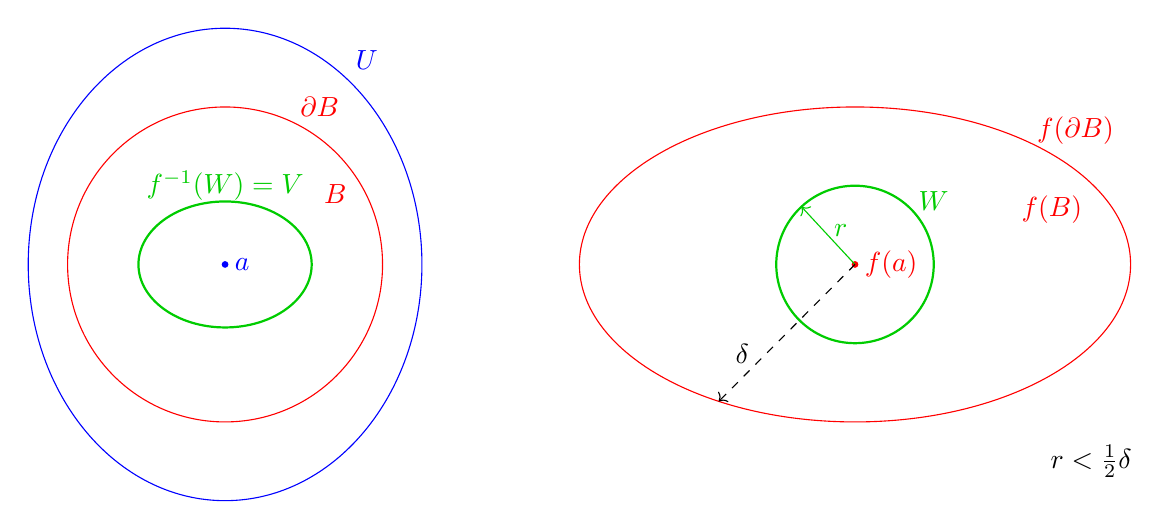
\begin{tikzpicture}
		\draw[red] (4,0) circle [x radius=3.5cm, y radius=2cm] node[xshift=2.8cm, yshift=1.7cm]{$f(\partial B)$} node[xshift=2.5cm, yshift=0.7cm]{$f(B)$} node[xshift=3cm,yshift=-2.5cm,black]{$r<\frac12\delta$};
		\draw[blue] (-4,0) circle [x radius=2.5cm, y radius=3cm] node[xshift=1.8cm, yshift=2.6cm]{$U$} ;
		\filldraw[blue] (-4,0) circle (1pt) node[anchor=west]{$a$};
		\filldraw[red] (4,0) circle (1pt) node[anchor=west]{$f(a)$};
		\draw[green!80!black,thick] (4,0) circle (1cm)  node[xshift=1cm,yshift=0.8cm]{$W$};
		\draw[green!80!black,thick] (-4,0) circle [x radius=1.1cm, y radius=0.8cm]node[xshift=0cm,yshift=1cm]{$f^{-1}(W)=V$};
		\draw[red] (-4,0) circle (2cm) node[xshift=1.2cm, yshift=2cm]{$\partial B$} node[xshift=1.4cm, yshift=0.9cm]{$ B$};
		\draw[green!80!black,->] (4,0) -- (3.32,0.733) node[xshift=5mm,yshift=-3mm] {$r$};
		\draw[dashed,->] (4,0) -- (2.27,-1.739) node[xshift=3mm, yshift=6mm]{$\delta$};
		
	\end{tikzpicture}
\end{center}
$\forall\ x\in B$ , $f'(x)$ is invertible. $\|r'(x)\|=\|f'(x)-f'(a)\|<\veps$. By $MVT$ applied on $r(x)$ on the convex set $B$, we get for any $x_1,x_2\in B$ $$\|f(x_1)-f(x_2)-f'(a)(x_1-x_2)\|=\|r(x_1)-r(x_2)\|\leq \veps \|x_1-x_2\|$$Now recall $\|p-q\|\geq \|p\|-\|q\|$. Hence $$\|f(x_1)-f(x_2)-f'(a)(x_1-x_2)\|\geq \|f'(a)(x_1-x_2)\|-\|f(x_1)-f(x_2)\|$$\textbf{Upshot: }$\|f(x_1)-f(x_2)\|\geq \|f'(a)(x_1-x_2)\|-\veps\|x_1-x_2\|\geq \overset{\substack{\text{Needed} \\ \downarrow}}{\cdots}$
\nt{At this point if we had normalized $f'(a)=$ Identity then we would have gotten $$\|f(x_1)-f(x_2)\|\geq (1-\veps)\|x_1-x_2\|$$ Taking $\veps<1$ fives the injectivity of $f$}\parinn

In our case we need to find lower bound on $\|f'(a)(x_1-x_2)\|$. Minimize $\{\|f'(a)u\|\mid \|u\|=1\}$. $f'(a)$ is continuous and the set of all unit vectors is compact. This set has a minimum, minimum=$m>0$ as it is invertible so $f'(\text{non zero vector})\neq 0$. 

Now take $\veps<m$ and then in the resulting ball $B$ we have \begin{equation}
	\|f(x_1)-f(x_2)\|\geq (m-\veps)\|x_1-x_2\|\label{eq1}
\end{equation}This gives the injectivity of $f$ on $B$. So we have the bijection $B\mathrel{\raisebox{2pt}{$\xrightarrow{\ \ \  f\ \ \ }$}
\llap{\raisebox{-2pt}{$\xleftarrow[f^{-1}=g]{}$}}}f(B)$. \eqref{eq1} is saying that any $y_1=f(x_1), y_2=f(x_2)$ in $f(B)$, i.e. $g(y_1)=x_1,g(y_2)=x_2$ $$\|g(y_1)-g(y_2)\|\leq \frac{1}{m-\veps}\|y_1-y_2\|$$ i.e. $g$ is uniformly continuous.

\item We have bijection of $f$ between $B$ and $f(B)$, $V$ is supposed to be open but we have taken open ball, so its open. Inverse of $f$ ($g$) is continuous so what left is $f(B)$ open\parinn

To show that $f$ is a local Homeomorphism it is enough to find an open ball $W$ around $f(a)$ with $W\subset f(B)$. Then we simply take $V=f^{-1}(W)$ which is open by continuity of $f$ and clearly $V\mathrel{\raisebox{2pt}{$\xrightarrow{f}$}
	\llap{\raisebox{-2pt}{$\xleftarrow[g]{}$}}}W$ are bijections just restrict $f,g$ from $B,f(B)$ respectively.

How to construct $W$? What radius to take around $W$? Stay away from $f(\partial B)$. $\delta=\min\{ \|f(x)-f(a)\| \mid x\in \partial B  \}>0$. Choose radius of $W$ to be $\frac12\delta$. We will be done if we show $W\subset f(B)$ i.e. given any $c\in W$ $\exs\ x^*\in B$ such that $f(x^*)=c$ ($x^*$ is necessarily unique, by injectivity).\parinf

\textbf{\textit{Idea: }}Consider the differentiable function $\begin{cases}
	B\to \bbR_{\geq 0}\\ x\mapsto \|f(x)-c\|^2
\end{cases}$\parinn


Note that $\|c-\text{ any point on }f(\partial B)\|>r$ by triangle inequality where as $\|c-f(a)\|<r$ (as $c$ is inside $W=$ ball of radius $r<\frac12\delta$ around $f(a)$). Hence $\|f(x)-c\|^2$ will take its minimum value at some point say $x^*\in B$. Now $f=(f_1,f_2,\dots,f_n)$ and $c=(c_1,\dots,c_n)$ $$\mu(x)=\|f(x)-c\|^2=\sum_{i=1}^n (f_i(x)-c_i)^2$$Derivative of this function is $0$ at $x^*$

\begin{center}
	\begin{tikzcd}
		B \arrow[r, "f"] & \bbR^n \arrow[ r, "\mu"] & \bbR \\
		x \arrow[r, maps to] & f(x)=y \arrow[r, maps to] & \|y-c\|^2
	\end{tikzcd}
\end{center}
Hence $$\EqM{c1}{\underbrace{\mu'(f(x^*))}}\circ f'(x^*)=0$$
\begin{tikzpicture}[remember picture, 
	overlay
	]
	\draw[<-] ++(c1.south) -- ++(0,-2em)  node[xshift=-1.6cm,yshift=-.6cm] {$\mat{2(f_1(x^*)-c_1) & \cdots & 2(f_n(x^*)-c_n)}$ (Matrix of $f'(x^*)$ -- Invertible) };
\end{tikzpicture}

\vspace{1.5cm}

Therefore $\mat{2(f_1(x^*)-c_1) & \cdots & 2(f_n(x^*)-c_n)}$ must be 0 i.e. $f_i(x^*)=c_i$ i.e. $f(x^*)=c$. So we showed that each $c\in W$ is in the image of $f$. Now take $V=f^{-1}(W)$ and we have the Homeomorphism.


\item Differentiability of $f^{-1}=g$ at any point $y\in W$.

\begin{center}
	\begin{tikzcd}
		x \arrow[r, rightharpoonup, "f",yshift=0.5mm] \arrow[d, bend right=25,"\text{add }h", swap] & y \arrow[l, rightharpoonup, "g", yshift=-0.5mm] \arrow[d, bend left=25, "\text{add }k"]  \\
		x+h \arrow[r, rightharpoonup, "f",yshift=0.5mm] & y+k\in W \arrow[l, rightharpoonup, "g", yshift=-0.5mm]
	\end{tikzcd}
\end{center}

Take small $k\in\bbR^n$ and let $h=g(y+k)-g(y)$ and $k=f(x+h)-f(x)$. Each of $h$ and $k$ determines the other uniquely. In particular $h\neq 0\iff k\neq 0$ (by bijectivity). $h\to 0 \iff k\to 0$ (by continuity of $f$ and $g$). $\alpha(h)=f(x+h)-f(x)-Th=k-Th$ where $T=f'(x)$. Then we have $\frac{\|\alpha(h)\|}{\|h\|}\to 0$ as $\|h\|\to 0$. We want to show $g'(y)=T^{-1}$

Let $\beta(k)=g(y+k)-g(y)-T^{-1}k=h-T^{-1}k$. We will show that as $k\to 0$, $\frac{\|\beta(k)\|}{\|k\|}\to 0$\begin{align*}
	\frac{\|\beta(k)\|}{\|k\|} = \frac{\|h-T^{-1}k\|}{\|k\|}= \frac{\|T^{-1}(Th-k)\|}{\|k\|} & \leq \frac{\|T^{-1}\|}{\|k\|}\|Th-k\|\\
	& = \frac{\|T^{-1}\|}{\|k\|} \|\alpha(h)\|\\
	& = \frac{\|T^{-1}\|}{\|k\|} \frac{\|\alpha(h)\|}{\|h\|}\|h\|\\
	& = \|T^{-1}\|\frac{\|h\|}{\|k\|}  \frac{\|\alpha(h)\|}{\|h\|}
\end{align*}
We know by $\frac{\|h\|}{\|k\|} <\frac{1}{m-\veps}$ by  \eqref{eq1}. $\frac{\|\alpha(h)\|}{\|h\|}\to 0$ as $k\to 0$ because then $h\to 0$.
\end{enumerate}
\end{proof}
\nt{\begin{itemize}
		\item For another proof of surjectivity onto $W$, see Rudin's use of contraction property
		\item There is a more general result which assumed only invertibility of $f'(x)$ for $x\in U$ but not continuity of $f'$ everywhere. (See exposition on Terence Tao's Blog: \url{https://terrytao.wordpress.com/tag/inverse-function-theorem/})
		\item $f$ need not be globally invertible!
		
		Example = See Problem 17 from Rudin
		
		$f(x,y)=(e^x\cos y,e^x\sin y)$. Then $$f'(x,y)=\mat{e^x\cos y & -e^x\sin y\\ e^x\sin y & e^x\cos y}\xrightarrow{\det}(e^x)^2(\cos^2x+\sin^2y)=e^{2x}>0$$Thus $f$ is locally invertible everywhere with $C^{1}$ inverse.
		\item $f$ is not globally one-one $f(x,y)=f(x,y+2\pi)$. Do the rest.
\end{itemize}}
\corc{}{If $f$ is a $C^1$ map from open $U$ in $\bbR^n$ to $\bbR^n$ and $f'(x)$ is invertible $\forall\ x\in U$ then\begin{enumerate}[label=\bfseries\tiny\protect\circled{\small\arabic*}]
		\item $f$ is an open map 
		\item $f$ is locally invertible with each such inverse a $C^1$ dunction (because matrix of $(f^{-1})'=$ inverse of matrix of $f'$ and entries of $A^{-1}=\frac1{\det A}$ (polynomials in entries of $A$) in particular $A\to A^{-1}$ is continuous)
\end{enumerate}}


\chapter{Implicit Function Theorem}
\textbf{Notation: }For $n>m$ let $n=m+d$. Write points of $\bbR^n=\bbR^d\times \bbR^m$ as $(x,y)$ where $x\in \bbR^d,$ $y\in \bbR^m$
\thmc[implicit]{Implicit Function Theorem}{
Let $U$ open in $\bbR^{d+m}$. $\Phi:U\to \bbR^m$ is a $C^1$ map such that $\Phi'(p)$ is surjective (which means columns of the $m\times (d+m)$ matrix of $\Phi'(p)$ span $\bbR^m$). WLOG suppose the last $m$ columns of $\Phi'(p) $ are linearly independent and hence span $\bbR^m$ i.e. the $m\times m$ matrix ``$\lt.\deld{\Phi}{y}\rt|_p=\mat{D_{d+1}\Phi(p) & \cdots & D_{d+m}\Phi(p)} $" is invertible. Then \begin{enumerate}
	\item $\exs$ a neighorhood $W$ of $a$ in $\bbR^d$ and a unique $C^1$ map $W\xrightarrow{f}\bbR^m$ such that $\begin{rcases}
		f(a)=b, (x,f(x))\in U\ \forall \ x\in W\text{ and}\\
		\Phi(x,f(x))=c\ \forall \ x\in W
	\end{rcases}$ i.e. $f$ is an implicit solution to the equation $\Phi(x,y)=c$
\item One can calculate $f'(x)$ by ``Implicit Differentiation"
\end{enumerate}
}
To understand this, first examine two cases:
\begin{itemize}
	\item When $\Phi$ is a linear map given by a matrix $A$. Here we are solving the equation $A\mat{x\\ y}=c$
	\item $d=m=1$ i.e. $n=2$ $\Phi(x,y)=x^2+y^2-1$, solving $\Phi(x,y)=0=c$. When $\lt.\deld{\Phi}{y}\rt|_{p=(a,b)}\neq 0$ we can locally solve for $y$ in terms of $x$ near $p$. $$D\Phi=\lt.\mat{\del{\Phi}{x} & \del{\Phi}{y}}\rt|_{(a,b)}=\mat{2a & 2b}$$ $2b=0$ at $(\pm 1,0)$
\end{itemize}
\begin{proof}
	We will choose $W$ later. Define \begin{center}
		\begin{tikzcd}
			U \arrow[r, "\psi"] & \bbR^{d+m}\\
			(x,y)\arrow[r, maps to] & (x, \Phi(x,y))
		\end{tikzcd}
	\end{center}
Note $\psi'$ has the matrix $\mat{I & O\\ \del{\Phi}{x} & \del{\Phi}{y}}$. This is nonsingular in a neighborhood of $p$. So by \hyperref[th:invthm]{Inverse Function Theorem} $\psi$ is invertible with $C^1$ inverse in a neighborhood $V$ of $p$
\begin{center}
	\begin{tikzcd}
		V \arrow[r] & \psi(V) \arrow[l]\\[-8mm]
		(a,b)\arrow[r, maps to] & (a,c)\\[-8mm]
		(x,y)\arrow[r, maps to] & (x,\Phi(x,y))\\[-8mm]
		(u,\alpha(u,v)) & (u,v) \arrow[l, maps to]
	\end{tikzcd}
\end{center}Definition of $\alpha(u,v)$ defined on $\psi(V)$. This tells us $\alpha(a,c)=b$. Whenever $\Phi(x,y)=c$ i.e. $$(x,y)\xrightarrow{\Phi}(x,c)\xrightarrow{\psi^{-1}}(x,\alpha(x,c))=(x,y)$$ i.e. $y=\alpha(x,c)$ and $\Phi(x,\alpha(x,c))=c$

So we are forced to define $f(x)=\alpha(x,c)$. But what should be the domain of this function $f$ i.e. what should we take $W$ to be. 

\begin{center}
	$(a,c)\in \psi(V)$ is open $\supset$ $\lt( \text{\begin{tabular}{c}
		open ball $W$ \\ around $a$ in $\bbR^d$
	\end{tabular}} \rt)\times \{c\} $
\end{center}

Now for any $x\in W$ we know $(x,c)\in \psi(V)$ i.e. $(x,\alpha(x,c))\in V$ so we define $f:W\to \bbR^m$ where $f(x)=\alpha(x,c)$ and we have derived the function. Now $\phi^{-1}$ is $C^1$ and $\alpha$ is component of $\phi^{-1}$ so all components of $\phi^{-1}$ is also $C^1$. hence $f$ is $C^1$

Uniqueness of $f$ is not true in general for arbitrary $W$. $\Phi(x,y)=x^2+y^2,\ c=1$. In $W=W_1\sqcup W_2$ $$f(x)=\begin{cases}
	\sqrt{1-x^2} & x\in W_1 \qquad[\text{is forced}]\\
	\sqrt{1-x^2} \text{ or }-\sqrt{1-x^2} & x\in W_2
\end{cases}$$. We have choice for $f$ on $W_2$. 

\textbf{If $W$ is connected, $f$ will be unique}. Eg. take $W$ to be a ball.  Suppose $g$ is another solution to $\Phi(x,y)=c$ i.e. $\Phi(x,g(x))=c$ for $x\in W$ and $g(a)=b$. Then consider the set $S=\{x\in W\mid f(x)=g(x)\}$. Show that this set is both closed (easy $S=(f-g)^{-1}(0)$) and open. 


Calculate derivative of $f$ using the fact that $\psi\circ \psi^{-1}=$ Identity and Chain Rule.
\end{proof}
\ex{Application of Implicit Function Theorem}{
\begin{enumerate}[label=(\roman*)]
	\item Linear map $\Phi:\bbR^{d+m}\to \bbR^m$ given by matrix $A$. Given $A\mat{a\\ b}=c$. Want to solve $A\mat{x\\ y}=c$
	
	$A=[P \mid Q]$ where $P$ is $m\times d$ and $Q$ is $m\times m$ and $Q$ is invertible. i.e. \begin{multline*}
		[P\mid Q]\mat{x\\ y}=c\iff [Q^{-1}P\mid I]\mat{x\\ y}=Q^{-1}c\iff Q^{-1}Px+y=Q^{-1}c\\
		\iff y=Q^{-1}c-Q^{-1}Px
	\end{multline*}
\item We can solve for $y$ in terms of $x$ near any $(a,b)$ on the unit circle when $\lt.\deld{\Phi}{y}\rt|_{(a,b)}\neq 0$. [This is mate when $b\neq 0$ i.e. at all points except $(\pm 1,0)$]. $$\lt.D\Phi\rt|_{(a,b)}=\mat{2a& 2b}$$ We can see directly 

\begin{center}
	$\begin{rcases}
		\text{when }b>0 & y=\sqrt{1-x^2}\\
		\text{when }b<0 & y=-\sqrt{1-x^2}
	\end{rcases}$ near (a,b) in fact $\forall\ x\in (-1,1)$
\end{center}
Similarly we can solve for $x$ in terms of $y$ when $\lt.\deld{\Phi}{x}\rt|_{(a,b)}=2a\neq 0$ This is true when $a\neq 0$
\end{enumerate}

}
\pagebreak
\textbf{\textit{Remark: }} Implicit Function Theorem gives a sufficient condition to be able to locally solve a system of linear equations \begin{center}
	$\begin{rcases}
		\Phi_1(x_1,\dots,x_d,y_1,\dots,y_m)=c_1\\
		\Phi_2(x_1,\dots,x_d,y_1,\dots,y_m)=c_1\\
		\qquad\vdots \qquad\qquad \vdots \qquad\qquad \vdots\\
		\Phi_m(x_1,\dots,x_d,y_1,\dots,y_m)=c_1
	\end{rcases}$\begin{tabular}{l}
	for $y_i$'s in terms of $x_i$'s \\
	locally near a given solution\\
	$y=b$ and $x=a$
\end{tabular}
\end{center}

\nt{
The condition of invertibility of submatrix of $\Phi$ is not necessary. Eg. $\Phi(x,y)=y-x^3$ near $(0,0)$ $$\lt.D\Phi\rt|_{(0,0)}=\lt. \mat{-3x^2 & 1}\rt|_{(0,0)}=\mat{0,1} \qquad \lt.\deld{\Phi}{x}\rt|{(0,0)}=0$$ but still we can solve for $x$ in terms of $y$: $x=\sqrt[3]{y}$ 
}

\chapter{Complex Differentiation}
Suppose $U$ open in $\bbC=\bbR^2$, $U\xrightarrow{f}\bbC$ a differentiable map i.e. $Df$ as an $\bbR$ linear operator $\bbR^2\to \bbR^2$ is defined. 

\nt{There is one thing that makes $\bbC$ differ from $\bbR^2$ i.e. $\bbC$ forms a field.}
\dfnc{Complex Differentiation}{
$f:U\to \bbC$ is called complex differentiable at $z_0\in U$ if $$\lim_{h\to 0} \frac{f(z_0+h)-f(z_0)}{h}\qquad \text{exists}$$ Thus the limit equals to $f'(z_0)$. $h$ is a complex number and this is a division in the field $\bbC$. `$h\to 0$' means $\|h\|\to 0$
}
\dfnc{Holomorphic Function}{We say that $f$ is holomorphic on $U$ if $f'(z)$ exists $\forall\ z\in U$. Then $f':U\to \bbC$ is the derivative of $f$ where $z\mapsto f'(z)$}

\thmc{}{$f$ is holomorphic $\iff$ so is $f'$}

\section*{Cauchy Riemann Conditions}
Suppose $f'(z_0) $ exists where $z_0=a+ib\in $ open $U\subset \bbC$. $f(z)=u+iv$ where $u:U\to \bbR$ and $v:U\to \bbR$. First take $h=t\in \bbR$. \begin{align*}
	f'(z_0) & = \lim_{t\to 0}\frac{f(a+t+ib)-f(a+ib)}{t}\\
	& = \lim_{t\to 0} \frac{u(a+t,b)-u(a,b)}{t}+i\lim_{t\to 0}\frac{v(a+t,b)-v(a,b)}{t}\\
	& = \lt.\del{u}{x}\rt|_{z_0}+i\lt. \del{v}{x}\rt|_{z_0} \numberthis\label{cd1}
\end{align*}
Now take $h=it$, $t\in \bbR$
\begin{align*}
	f'(z_0) & = \lim_{t\to 0}\frac{f(a+ib+it)-f(a+ib)}{it}\\
	& = \lim_{t\to 0} \frac{u(a,b+t)-u(a,b)}{it}+i\lim_{t\to 0}\frac{v(a,b+t)-v(a,b)}{it}\\
	& = \frac1i \lt[ \lt.\del{u}{y}\rt|_{z_0} + i \lt. \del{v}{y}\rt|_{z_0} \rt]\\
	& = \lt. \del{v}{y}\rt|_{z_0} -i\lt. \del{u}{y}\rt|_{z_0}\numberthis\label{cd2}
\end{align*}
Equating \eqref{cd1}  and \eqref{cd2} $f$ is complex differentiable at $z_0$ and $$\boxed{\lt.\del{u}{x}\rt|_{z_0}=\lt.\del{v}{y}\rt|_{z_0}\qquad \lt.\del{v}{x}\rt|_{z_0}=-\lt.\del{u}{y}\rt|_{z_0}}$$


In fact more is true.
\begin{Claim}{}{}
	For open $U\subset \bbC$ if $U\xrightarrow{f}\bbC$ is complex differentiable at $z_0\in U$ then $f$ is also real differentiable as a function $U\to \bbR^2$ and its Jacobin is (letting $f=(u,v)$, $u,v:U\to \bbR$)
	$$Jf(z_0)=\lt. \mat{\del{u}{x} & \del{u}{y}\\ \del{v}{x} & \del{v}{y}} \rt|_{z_0} =\lt. \mat{\del{u}{x} & \del{u}{y}\\ -\del{u}{y} & \del{u}{x}} \rt|_{z_0} = \lt. \mat{\del{v}{y} & -\del{v}{x}\\ \del{v}{x} & \del{v}{y}} \rt|_{z_0}$$
\end{Claim}

\end{document}
